\documentclass[11pt]{article}
\usepackage[paperwidth=160mm,paperheight=90mm,margin=7mm,top=6mm,bottom=6mm]{geometry}
\usepackage{amsmath,amssymb,mathtools}
\usepackage{booktabs}
\usepackage{tikz}
\usetikzlibrary{arrows.meta,positioning,calc}
\usepackage{xcolor}
\usepackage{enumitem}
\usepackage[hidelinks]{hyperref}
\definecolor{arb}{RGB}{27,94,52}
\definecolor{arbred}{RGB}{150,40,40}
\definecolor{arbdim}{RGB}{100,100,100}
\setlist{nosep,leftmargin=*}
\pagestyle{empty}
\setlength{\parindent}{0pt}
\setlength{\parskip}{3pt}
\newcommand{\F}{\mathbb{F}}
\newcommand{\G}{\mathbb{G}}
\newcommand{\Ep}{\ensuremath{\mathcal{E}}}
\newcommand{\Pallas}{\ensuremath{\mathsf{Pallas}}}
\newcommand{\Vesta}{\ensuremath{\mathsf{Vesta}}}
\newcommand{\Fpp}{\ensuremath{\F_{p_{\Pallas}}}}
\newcommand{\Fpv}{\ensuremath{\F_{p_{\Vesta}}}}
\newcommand{\nfsym}{\ensuremath{\mathsf{nf}}}
\newcommand{\cmsym}{\ensuremath{\mathsf{cm}}}
\newcommand{\cmx}{\ensuremath{\mathsf{cmx}}}
\newcommand{\cvsym}{\ensuremath{\mathsf{cv}}}
\newcommand{\rksym}{\ensuremath{\mathsf{rk}}}
\newcommand{\gd}{\ensuremath{\mathsf{g_d}}}
\newcommand{\pkd}{\ensuremath{\mathsf{pk_d}}}
\newcommand{\aksym}{\ensuremath{\mathsf{ak}}}
\newcommand{\nksym}{\ensuremath{\mathsf{nk}}}
\newcommand{\asksym}{\ensuremath{\mathsf{ask}}}
\newcommand{\ivk}{\ensuremath{\mathsf{ivk}}}
\newcommand{\fvk}{\ensuremath{\mathsf{fvk}}}
\newcommand{\ovk}{\ensuremath{\mathsf{ovk}}}
\newcommand{\dk}{\ensuremath{\mathsf{dk}}}
\newcommand{\rcm}{\ensuremath{\mathsf{rcm}}}
\newcommand{\rcv}{\ensuremath{\mathsf{rcv}}}
\newcommand{\rivk}{\ensuremath{\mathsf{r_{ivk}}}}
\newcommand{\rsk}{\ensuremath{\mathsf{rsk}}}
\newcommand{\esk}{\ensuremath{\mathsf{esk}}}
\newcommand{\epk}{\ensuremath{\mathsf{epk}}}
\newcommand{\Extract}{\ensuremath{\mathsf{Extract}}}
\newcommand{\NoteCommit}{\ensuremath{\mathsf{NoteCommit}}}
\newcommand{\GroupHash}{\ensuremath{\mathsf{GroupHash}}}
\newcommand{\CommitIvk}{\ensuremath{\mathsf{Commit}^{\mathsf{ivk}}}}
\newcommand{\Comm}{\ensuremath{\mathsf{Commit}}}
\newcommand{\ip}[2]{\langle #1,\, #2 \rangle}
% Sources are not shown on screen.
\newcommand{\src}[1]{}
% One board per screen.
\newcounter{board}
\newsavebox{\bdlabel}
\newenvironment{board}[2]{\clearpage\stepcounter{board}%
  \sbox{\bdlabel}{\small\color{arbdim}#2}%
  \noindent\parbox[b]{\dimexpr\textwidth-\wd\bdlabel-1em\relax}{\raggedright
    \color{arb}\large\bfseries #1}\hfill\usebox{\bdlabel}\par
  \vspace{2pt}{\color{arb!40}\hrule}\vspace{4pt}}{\par}
% A part title becomes a divider screen.
\RenewDocumentCommand{\section}{s o m}{\clearpage\vspace*{\fill}%
  \begin{center}{\color{arb}\LARGE\bfseries #3}\end{center}\vspace*{\fill}\clearpage}
\makeatletter
\newcommand{\shead}[1]{\par\smallskip{\small\bfseries\color{arbdim}#1}\par\nopagebreak}
\makeatother
\newcommand{\Write}{\shead{Write}}
\newcommand{\Say}{\shead{Say}}
\newcommand{\Ask}{\shead{Ask}}
\newcommand{\Answer}{\clearpage\shead{Answer}}
\newcommand{\Fig}[1]{\begin{center}\resizebox{!}{\dimexpr\textheight-42pt\relax}{#1}\end{center}}
\title{Zcash for Bitcoiners}
\author{}
\date{}

\begin{document}
%% ---- 01-opening.tex
%% Part A --- screen version of wb/01-opening.tex.

\section{Part A --- What Bitcoin publishes, and what privacy must mean}

\begin{board}{Alice pays Bob in Bitcoin: what the chain publishes}{all four}
\Write
{\centering
\resizebox{!}{0.45\textheight}{%
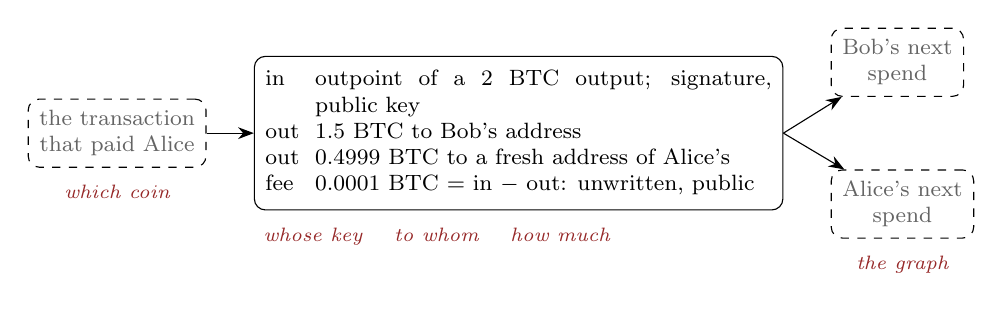
\begin{tikzpicture}[>={Stealth[length=2mm]}, font=\footnotesize,
  box/.style={draw, rounded corners, inner sep=4pt, align=left},
  ext/.style={draw, dashed, rounded corners, inner sep=4pt, align=center,
    text=arbdim},
  tag/.style={font=\scriptsize\itshape, text=arbred, align=center}]
\node[box] (tx) {\hyphenpenalty=10000 \begin{tabular}{@{}l@{\ \ }p{58mm}@{}}
  in  & outpoint of a $2$ BTC output; signature, public key \\
  out & $1.5$ BTC to Bob's address \\
  out & $0.4999$ BTC to a fresh address of Alice's \\
  fee & $0.0001$ BTC $=$ in $-$ out: unwritten, public \\
\end{tabular}};
\node[ext, left=6mm of tx] (prev) {the transaction\\ that paid Alice};
\node[ext, right=6mm of tx.east, yshift=9mm] (bobnext) {Bob's next\\ spend};
\node[ext, right=6mm of tx.east, yshift=-9mm] (alnext) {Alice's next\\ spend};
\draw[->] (prev) -- (tx);
\draw[->] (tx.east) -- (bobnext);
\draw[->] (tx.east) -- (alnext);
\node[tag, below=1mm of prev] {which coin};
\node[tag, below=1mm of alnext] {the graph};
\node[tag, below=1mm of tx.south west, anchor=north west]
  {whose key \quad to whom \quad how much};
\end{tikzpicture}}\par}
\Say
Nobody wrote ``Alice'' or ``Bob'' on the chain, but which coin, whose key,
to whom, how much and the spend graph are all in the record; the unwritten
fee is public. Address reuse merges a history; the non-round change output
to a fresh address is usually the payer's. The shielded running example
has this shape, with none of the labels.
\end{board}

\begin{board}{The validator's four checks}{all four}
\Write
{\small
\begin{tabular}{@{}l@{\qquad}l@{\qquad}l@{}}
  \texttt{validate(tx):} & & \\
  \texttt{\ \ for input in tx.inputs:} & & \\
  \texttt{\ \ \ \ coin = utxo[input.prev\_out]}
    & (1) coin exists & reads the outpoint \\
  \texttt{\ \ \ \ check sig(input.sig, coin.script)}
    & (2) authorised & reads script and key \\
  \texttt{\ \ \ \ delete utxo[input.prev\_out]}
    & (3) not spent twice & reads the outpoint \\
  \texttt{\ \ check sum(in) >= sum(out)}
    & (4) conserved & reads every amount \\
\end{tabular}}

fee $= \Sigma\,\mathrm{in} - \Sigma\,\mathrm{out}$
\Say
In Bitcoin the whole state is one table, the set of unspent outputs; a
spend is a lookup, a signature check and a deletion. Every check reads a
plaintext field of the transaction or of the output it names: nothing is
inferred. The fee is check 4's slack: not a field, yet public to the
satoshi. These four numbers are the spine of the workshop; every later
board names the check it serves.
\end{board}

\begin{board}{Hide a field, lose a check}{all four}
\Write
\begin{itemize}
  \item hide the amount $\to$ check 4 dies: nothing to add up
  \item hide the input reference $\to$ checks 1 and 3 die: nothing to look
    up, nothing to delete
  \item hide the key $\to$ check 2 dies: nothing to verify against
  \item hide the receiver $\to$ nothing dies here: the output's script is
    what check 2 reads when Bob spends it, so that spend's check 2 dies
\end{itemize}
\medskip
\fbox{\parbox{\dimexpr\textwidth-2\fboxsep-2\fboxrule\relax}{%
  \emph{Privacy, for this workshop: hide the sender, the receiver and
  the amount, while a stranger still performs all four checks.}}}
\Say
Every mechanism to come answers the same pair of questions: which of the
four checks does it restore, and why can the node no longer do it the
Bitcoin way?
\end{board}

\begin{board}{What a privacy design must supply}{all four}
\Write
{\small\setlength{\tabcolsep}{4pt}
\begin{tabular}{@{}p{40mm}p{62mm}p{36mm}@{}}
  \toprule
  \emph{the validator must} & \emph{the tool} & \emph{Bitcoin's version} \\
  \midrule
  accept a claim about data it cannot see
    & a zero-knowledge proof: the statement public, the witness (the
      prover's secret input, not Bitcoin's witness field) private
    & look at the data \\
  know the hidden data cannot change under it
    & a commitment: hiding, and binding
    & the output, in the clear \\
  notice the same hidden coin a second time
    & a nullifier: a keyed, one-way tag of the coin, published at spend
    & delete it from the set \\
  add up amounts it cannot read
    & a homomorphic commitment: sealed envelopes that add
    & add the numbers \\
  \bottomrule
\end{tabular}}

\emph{the proof checks the claim; the other three tools make the claim
about something fixed, unrepeatable, summable.}
\end{board}

\begin{board}{Sealed envelopes that add}{conserved}
\Write
\[
\bigl([v_1]\,V + [r_1]\,R\bigr) + \bigl([v_2]\,V + [r_2]\,R\bigr)
  = [v_1 + v_2]\,V + [r_1 + r_2]\,R
\]
\emph{holds modulo the group order; the $64$-bit range check lives inside
the proof.}
\Say
Two commitments add without either being opened: the two sealed
envelopes combine into an envelope for the sum of the values, with the
sum of the randomness. It is the Confidential Transactions trick: amounts
hidden, their sum still checkable.
\end{board}

\begin{board}{Notes versus UTXOs: what a coin is}{authorised, conserved}
\Write
{\small\setlength{\tabcolsep}{4pt}
\begin{tabular}{@{}p{32mm}p{52mm}p{54mm}@{}}
  \toprule
  & \emph{Bitcoin UTXO} & \emph{Zcash note} \\
  \midrule
  owner
    & a script, usually one key hash, on chain
    & an address $(d, \pkd)$, inside the note \\
  value
    & the amount, on chain
    & $v \in [0, 2^{64})$ zatoshi, inside the note \\
  spending condition
    & script: signatures, timelocks, hashlocks
    & a key, full stop --- no script, no timelocks, no HTLCs \\
  \bottomrule
\end{tabular}}
\Say
In Zcash both owner and value are fields of the note, and the note is
never published. Threshold authority exists and is invisible on chain: it
is FROST, later in the workshop; on chain there is one ordinary signature
under one per-spend key.
\end{board}

\begin{board}{Notes versus UTXOs: what the chain records}{exists, not twice}
\Write
{\small\setlength{\tabcolsep}{4pt}
\begin{tabular}{@{}p{32mm}p{46mm}p{60mm}@{}}
  \toprule
  & \emph{Bitcoin UTXO} & \emph{Zcash note} \\
  \midrule
  on-chain identifier
    & the outpoint
    & a commitment $\cmsym$ to the note, stored as $\cmx$ \\
  spent marker
    & removed from the UTXO set
    & a nullifier $\nfsym$, published at spend \\
  set structure
    & one set: insert, delete
    & an append-only tree of $\cmx$, depth $32$, and a set of $\nfsym$:
      append only, both \\
  \bottomrule
\end{tabular}}

\emph{the note never touches the chain.}
\Say
Nothing is ever deleted. Recorded are a commitment to the note, an
encrypted copy for its recipient, and at spend a tag derived from it.
\end{board}

\begin{board}{The three-line mental model}{all four}
\Write
A shielded spend is three claims about a note nobody sees:
\begin{enumerate}
  \item \emph{it exists} --- a commitment to it is a leaf under a public
    root, proved with leaf, position and path all private;
  \item \emph{it is spent now} --- its serial number, the nullifier, is
    revealed, and the chain refuses to see it twice;
  \item \emph{the books balance} --- commitments to the amounts add up to
    the declared net flow.
\end{enumerate}
\setlength{\abovedisplayskip}{4pt}\setlength{\belowdisplayskip}{4pt}
\[
R_{\mathrm{mem}} = \bigl\{\, (\underbrace{\mathit{rt}}_{\text{public}};\
  \underbrace{(\cmx,\ i,\ \mathit{path})}_{\text{private}}) \ :\
  \mathsf{Verify}(\mathit{rt}, i, \cmx, \mathit{path}) = \mathsf{accept}
  \,\bigr\}
\]
\Say
A Bitcoin spend names its coin and signs; a shielded spend names nothing:
it proves line 1, reveals line 2 and signs for line 3, under a key the
proof ties to the note (check 2). Everything else in the workshop is
machinery for these three lines and that signature.
\end{board}

\begin{board}{Four checks, four mechanisms}{all four}
\Write
{\small\setlength{\tabcolsep}{4pt}
\begin{tabular}{@{}p{7mm}p{24mm}p{38mm}p{64mm}@{}}
  \toprule
  & \emph{the check} & \emph{Bitcoin} & \emph{shielded Zcash} \\
  \midrule
  (1) & coin exists
    & look the outpoint up in the UTXO set
    & a commitment in an append-only tree; a membership proof under a
      public root \\
  (3) & not spent twice
    & delete it from the set
    & a nullifier, published once, refused the second time \\
  (4) & conserved
    & add the amounts up
    & value commitments that add; a binding signature over their sum \\
  (2) & authorised
    & run the script over the signature
    & key knowledge proved inside the proof; a signature under a
      re-randomised key \\
  \bottomrule
\end{tabular}}
\Say
Each part of the workshop reopens with both questions: which check, and
why not the Bitcoin way (settled on ``Hide a field, lose a check'').
Checks 1 and 3 come first, with the data model; checks 4 and 2 follow.
\end{board}

\begin{board}{The route}{all four}
\Write
{\small
\begin{enumerate}
  \item \textbf{The toolbox} --- each primitive from the Bitcoin instance
    the room already holds.
  \item \textbf{The data model} --- notes, commitments, the tree, the
    nullifier: checks 1 and 3.
  \item \textbf{Keys and addresses} --- who can spend, who can see.
  \item \textbf{The Action statement} --- what the proof proves, clause by
    clause; then a break.
  \item \textbf{Balance and authority} --- checks 4 and 2, on the running
    example.
  \item \textbf{The proof system} --- from a statement to a few kilobytes.
  \item \textbf{Delivery and light clients} --- how Bob finds his money.
  \item \textbf{The transaction and the turnstile} --- the bytes on the
    chain, and the pools.
  \item \textbf{Consensus} --- why one fork wins, what the chain must
    remember.
  \item \textbf{Limits, frontier, takeaways.}
\end{enumerate}}

\emph{one example threads it: Alice pays Bob $1.5$ ZEC from a $2$ ZEC
note.}
\Ask
\emph{Which of the four checks does a nullifier serve, and what breaks if
two different notes could share one?}
\Answer
\begin{itemize}
  \item Check 3, not spent twice. The nullifier is ``delete from the UTXO
    set'' without naming the coin: published once, refused the second
    time.
  \item Two notes, one nullifier: whichever is spent first burns the other,
    and the second owner's honest spend is refused as a double spend ---
    an attack on earlier designs, in which forged notes could be made to
    share one.
  \item How the chain makes sure no two accepted notes can share one ---
    every new note inherits, as its seed, the serial of the note spent
    beside it --- is Part C's business.
\end{itemize}
\end{board}

%% ---- 02-toolbox.tex
%% Part B --- screen version of wb/02-toolbox.tex.

\section{Part B --- The toolbox, from Bitcoin's primitives up}

%% ---------------------------------------------------------------- B1
\begin{board}{Hash functions: one primitive, three notions}{all four}
\Write
\begin{enumerate}
  \item $H \colon \{0,1\}^{*} \to \{0,1\}^{n}$ --- fixed, public,
    compresses
  \item preimage: given $y$, find $x'$ with $H(x') = y$
  \item second preimage: given $x$, find $x' \ne x$ with $H(x') = H(x)$
  \item collision: find any $x \ne x'$ with $H(x) = H(x')$ --- strongest;
    commitments, Merkle trees, Fiat--Shamir
  \item generic: collision $\approx 2^{n/2}$ (birthday), preimage
    $\approx 2^{n}$; $n = 256 \Rightarrow 2^{128}$; RIPEMD-160
    $\Rightarrow 2^{80}$
  \item Bitcoin: SHA-256d (headers, txids);
    $\mathsf{hash160} = \mathrm{RIPEMD160} \circ \mathrm{SHA256}$
    (addresses)
  \item Zcash: keeps all of these (transparent) $+$ three shielded hashes
\end{enumerate}
\newpage
\Say
In the collision game the adversary picks both inputs, so it is the
strongest demand --- the one commitments, Merkle trees and Fiat--Shamir
need. The generic costs set the digest sizes. Nothing is taken away:
Zcash keeps every Bitcoin hash in its transparent layer and adds three
for the shielded one.
\Ask
Which of the three notions do commitments and Merkle trees lean on?
\Answer
Collision resistance: the adversary picks both inputs.
\end{board}

\begin{board}{Zcash's hashes: SHA-256 is not replaced}{all four}
\Write
{\small\setlength{\tabcolsep}{4pt}
\begin{tabular}{@{}lp{50mm}p{72mm}@{}}
  \toprule
  \emph{hash} & \emph{kind} & \emph{deployed use} \tabularnewline
  \midrule
  SHA-256d
    & bit-oriented, Bitcoin's
    & \raggedright header difficulty filter (after Equihash);
      transparent layer: legacy txids, Base58Check \tabularnewline
  BLAKE2b
    & \raggedright bit-oriented; personalised natively, the key
      prepended to the input
    & \raggedright $\mathsf{PRFexpand}$ (the key tree); note-encryption
      KDF; ZIP-244 digests (txid, sighash) \tabularnewline
  Poseidon
    & algebraic: $x \mapsto x^{5}$ over $\Fpp$
    & the nullifier PRF, inside the circuit \tabularnewline
  Sinsemilla
    & \raggedright algebraic: curve additions on \Pallas{}
    & \raggedright note commitment; Merkle node hash, both inside the circuit
      \tabularnewline
  \bottomrule
\end{tabular}}
\newpage
\Write
\begin{enumerate}
  \item Bitcoin's hashes stay where Bitcoin put them
  \item shielded: $+1$ bit-oriented (off the circuit), $+2$ algebraic
    (inside it)
\end{enumerate}
\Say
SHA-256d is not replaced: it keeps the header difficulty filter and the
transparent layer. The split is by where the work happens: BLAKE2b off
the circuit; Poseidon and Sinsemilla inside it.
\end{board}

\begin{board}{Why in-circuit hashing wants algebraic hashes}{exists,
  not twice}
\Write
\begin{enumerate}
  \item proof $=$ polynomial constraints over a prime field; field
    multiplication $=$ 1 constraint; Boolean operation $=$ several $+$
    range checks
  \item SHA-256, BLAKE2: 32-/64-bit words, XOR, shuffles $\Rightarrow$ tens
    of thousands of constraints per evaluation
  \item Poseidon round: $+$ constants; $x^{5}$ (all elements in a full
    round, one in a partial); $\times$ fixed matrix. 2-to-1 hash $\approx$
    a few hundred constraints. Orchard: width 3, 8 full $+$ 56 partial
  \item Sinsemilla, per 10-bit chunk: 1 lookup (table of $2^{10} = 1024$
    points) $+$ 2 incomplete additions; collision $\Rightarrow$ discrete
    log
\end{enumerate}
\newpage
\Say
A zero-knowledge proof re-expresses every step of a computation as
polynomial constraints over a prime field. SHA-256 and BLAKE2 are foreign
to the field; Poseidon keeps the only non-linear step at $x^{5}$;
Sinsemilla is curve arithmetic, native to the circuit. Bitcoin never
hashes inside a proof; the first shielded generation did, with SHA-256,
and its prover paid for it.
\end{board}

%% ---------------------------------------------------------------- B2
\begin{board}{Curves: the same shape, different primes}{all four}
\Write
\begin{enumerate}
  \item $y^{2} = x^{3} + b$ over a prime field; prime-order group, cofactor
    $1$; discrete log $=$ the standing assumption
  \item secp256k1: $b = 7$, $p = 2^{256} - 2^{32} - 977$, $256$-bit prime
    order
  \item \Pallas{}, \Vesta{}: $b = 5$, two $255$-bit primes $p_{\Pallas}$,
    $p_{\Vesta}$; $\#\Pallas = p_{\Vesta}$, $\#\Vesta = p_{\Pallas}$;
    $\approx 126$ bits of DL security
  \item generators: hashed to the curve (secp256k1's base point: a SEC~2
    constant)
  \item \Pallas{}: every point in an Action; \Vesta{}: the proof's
    polynomial commitments
\end{enumerate}
\Say
The scalar field of each Pasta curve is the base field of the other.
Every \Pallas{} and \Vesta{} generator the protocol uses is hashed to the
curve, so no relation between any two is known to anyone and there is no
ceremony for this stack; the Sapling pool still rests on its Groth16 MPC.
\end{board}

\begin{board}{Why not secp256k1: two-adicity}{all four}
\Write
{\small\setlength{\tabcolsep}{6pt}
\begin{tabular}{@{}lrrr@{}}
  \toprule
  \emph{field} & \emph{bits} & \emph{two-adicity of $p - 1$}
    & \emph{largest power-of-two domain} \\
  \midrule
  \Pallas{} base field   & $255$ & $32$ & $2^{32}$ \\
  \Vesta{} base field    & $255$ & $32$ & $2^{32}$ \\
  secp256k1 base field   & $256$ & $1$  & $2$ \\
  secp256k1 scalar field & $256$ & $6$  & $64$ \\
  \bottomrule
\end{tabular}}
\begin{enumerate}
  \item $2^{k}$-th roots of unity exist iff $2^{k} \mid p - 1$; largest
    such $k$ $=$ two-adicity
  \item Orchard circuit: $2^{11}$ rows
  \item secp256k1 rows: our own computation, not a volume figure
\end{enumerate}
\Say
A proof system of the PLONK family interpolates each circuit column over
the $2^{k}$-th roots of unity of its field. Neither secp256k1 field offers
a domain of $2^{11}$; the Pasta primes were searched for with two-adicity
$32$ and the cycle as design goals.
\Ask
Which secp256k1 field could host $2^{11}$ rows?
\Answer
Neither: the largest domains are $2$ and $64$.
\end{board}

%% ---------------------------------------------------------------- B3
\begin{board}{Commitments: a sealed envelope}{exists, conserved}
\Write
\begin{enumerate}
  \item $c = \Comm(m; r)$, trapdoor $r$; hiding: two candidate $m$
    indistinguishable from $c$; binding: no $c$ opens to two $m$
  \item not both perfect; deployed: perfectly hiding, binding under DL
  \item $\Comm(v; r) := [v]\,V + [r]\,R$, with $V, R$ hashed to \Pallas{}
  \item uniform $r \Rightarrow$ uniform point; two openings $\Rightarrow
    \log_{V} R$
  \item Bitcoin: CT's envelope; an address $=$ hash commitment to a
    key/script, opened at spend
  \item Zcash: $\cvsym$ seals the value change (Pedersen, adds); $\cmsym$
    seals the whole note (algebraic hash $+ [\rcm]\,H_{D}$)
\end{enumerate}
\newpage
\Say
Hiding: for uniform $r$ the point is uniform whatever $v$ is. Binding:
two openings of one $c$ solve $\log_{V} R$, which nobody holds. The note
commitment's blinding term $[\rcm]\,H_{D}$ has the same Pedersen shape
over its own hashed generator, so the circuit recomputes it cheaply.
\Ask
Can the envelope be perfectly hiding and perfectly binding at once?
\Answer
No; the deployed ones are perfectly hiding and binding under the discrete
logarithm.
\end{board}

\begin{board}{The envelope adds: the Confidential Transactions
  bridge}{conserved}
\Write
\begin{enumerate}
  \item $\Comm(v_{1}; r_{1}) + \Comm(v_{2}; r_{2})
    = \Comm(v_{1} + v_{2};\ r_{1} + r_{2})$
  \item \[
      \sum \Comm_{\mathrm{in}} - \sum \Comm_{\mathrm{out}}
      = \Bigl[\sum v_{\mathrm{in}} - \sum v_{\mathrm{out}}\Bigr] V
        + [\bar r]\,R
    \]
  \item $V$ term vanishes iff values balance --- modulo the group order;
    range check on every value closes the wrap
  \item CT (Elements): same equation on chain; range proof beside each
    commitment; receiver told the opening; amounts hidden, keys and graph
    clear
  \item here: $64$-bit range check $+$ opening $(v, \rcv)$ $=$ clauses of
    one ZK proof; net trapdoor $\bar r \to$ a signing key
\end{enumerate}
\newpage
\Say
Sum the inputs, subtract the outputs: the $V$ term carries
$\sum v_{\mathrm{in}} - \sum v_{\mathrm{out}}$ and vanishes exactly when
the values balance. Confidential Transactions checks this equation on the
chain; here it moves inside the proof, and the net trapdoor $\bar r$
becomes a signing key (board \emph{Preview: a signature under a key
nobody holds unless the values balance}).
\end{board}

%% ---------------------------------------------------------------- B4
\begin{board}{Merkle trees: from the txid tree to the note commitment
  tree}{exists}
\Write
{\centering
\resizebox{!}{0.6\textheight}{%
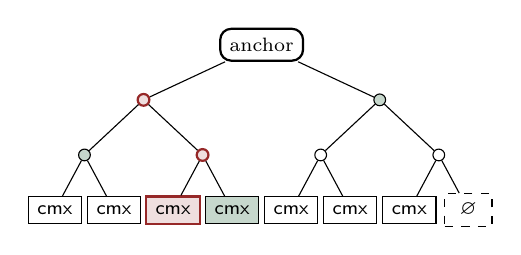
\begin{tikzpicture}[every node/.style={font=\scriptsize},level distance=7mm,
  level 1/.style={sibling distance=30mm},
  level 2/.style={sibling distance=15mm},
  level 3/.style={sibling distance=7.5mm},
  nd/.style={draw,circle,inner sep=1.5pt},
  lf/.style={draw,minimum width=6mm},
  rt/.style={draw=arbred,thick,fill=arbred!15},
  sb/.style={fill=arb!25}]
\node[draw,rounded corners,thick] {anchor}
  child {node[nd,rt] {}
    child {node[nd,sb] {}
      child {node[lf] {\cmx}}
      child {node[lf] {\cmx}}}
    child {node[nd,rt] {}
      child {node[lf,rt] {\cmx}}
      child {node[lf,sb] {\cmx}}}}
  child {node[nd,sb] {}
    child {node[nd] {}
      child {node[lf] {\cmx}}
      child {node[lf] {\cmx}}}
    child {node[nd] {}
      child {node[lf] {\cmx}}
      child {node[lf,dashed] {$\varnothing$}}}};
\end{tikzpicture}}\par
{\small\color{arbdim}red: the leaf and its route, private; green: the
siblings, private; the anchor alone is public\par}}
\newpage
\Write
\begin{enumerate}
  \item Bitcoin: txids pairwise up to the header root; SPV proof $=$ leaf
    $+$ one sibling per level; the leaf (txid) is public
  \item Zcash: leaves $= \cmx$ in creation order; depth $32$, room for
    $2^{32}$ notes; node hash Sinsemilla, tagged with its layer; root after
    each block $=$ that block's \emph{anchor}
  \item membership proof: $32$ siblings $+$ $32$ direction bits, verified
    by $32$ hashes --- inside the proof
\end{enumerate}
\Say
Bitcoin's SPV proof is the leaf plus one sibling per level, and the leaf
is public. Here the $32$ hashes are recomputed inside the proof: the
leaf, its route and the siblings stay private; the anchor alone is
public.
\end{board}

\begin{board}{What changes: append only, historical roots, private
  path}{exists}
\Write
\begin{enumerate}
  \item append only: one leaf at a time; frontier $\le 32$ carried labels;
    root updated in $32$ hashes; nothing deleted --- ``deleted'' $=$ a
    separate set
  \item history binding: proof against the root at insertion valid
    forever; consensus accepts the anchor of any earlier main-chain block
  \item private path: (leaf, index, siblings) $=$ witness; anchor $=$
    statement
  \item \[
      R_{\mathrm{mem}} = \bigl\{\,(\mathit{rt};\ (\cmx, i, \mathit{path})) :
        \mathsf{Verify}(\mathit{rt}, i, \cmx, \mathit{path})
        = \mathsf{accept}\,\bigr\}
    \]
  \item Bitcoin SPV names the txid; this proof names only the root
\end{enumerate}
\Say
Revealing (leaf, index, siblings) would say which note is spent, so the
path is a witness and only the anchor a statement. An SPV proof names
the txid it proves; this one hides the leaf among every leaf beneath it.
\end{board}

%% ---------------------------------------------------------------- B5
\begin{board}{Pseudorandom functions: a key that fakes randomness}{not
  twice}
\Write
\begin{enumerate}
  \item $F_{k}$ pseudorandom: secret uniform $k$; no efficient adversary
    with oracle access (any inputs, adaptively) tells $F_{k}$ from a
    random function
  \item algorithm public; only $k$ hidden; adversary sees input--output
    pairs, never $k$
  \item Bitcoin: HMAC-SHA512 in BIP-32 child derivation
  \item Zcash, off circuit: BLAKE2b personalised $= \mathsf{PRFexpand}$;
    $\mathsf{sk} \to \asksym, \nksym, \rivk$; later the note's randomness
    from its seed
  \item Zcash, in circuit: $F_{\nksym}(\rho) = \mathsf{PoseidonHash}(\nksym,
    \rho)$ over $\Fpp$; width $3$, S-box $x^{5}$, $8$ full $+$ $56$
    partial rounds
\end{enumerate}
\Say
Bitcoin already trusts a PRF to make BIP-32 child keys look unrelated.
Off the circuit, one $\mathsf{PRFexpand}$ call per sub-secret builds the
key ladder (Part D). Inside it, Poseidon is keyed by its first input:
$\nksym$ first, $\rho$ second.
\end{board}

\begin{board}{What a nullifier needs from a PRF}{not twice}
\Write
\begin{enumerate}
  \item \[
      \nfsym = \Extract\bigl([\,F_{\nksym}(\rho) + \psi\,]\,G^{\mathsf{nf}}
        + \cmsym\bigr)
    \]
  \item $\Extract$: the $x$-coordinate; $\rho, \psi$: per-note randomness
    fixed at creation; $G^{\mathsf{nf}}$: a hashed generator
  \item uniqueness: all inputs fixed once the note exists $\Rightarrow$
    deterministic; two notes, one tag $\Rightarrow$ DL relation on
    \Pallas{}; no PRF property used (forger holds $\nksym$)
  \item unlinkability: without $\nksym$, $[F_{\nksym}(\rho) + \psi]\,
    G^{\mathsf{nf}}$ masks $\cmsym$ --- Poseidon PRF or DDH on \Pallas{};
    either suffices
  \item Bitcoin: spent marker $=$ the outpoint, unique and public
\end{enumerate}
\newpage
\Say
Uniqueness uses no PRF property: every input is fixed once the note
exists, and the forger holds $\nksym$. Unlinkability does: without
$\nksym$ the masking term looks random. Bitcoin's spent marker is the
outpoint, unique and public; a nullifier must be unique \emph{and} say
nothing --- two separate properties.
\Ask
Which of the two properties uses the PRF?
\Answer
Only unlinkability; uniqueness is discrete-log structure, and the forger
holds $\nksym$ anyway.
\end{board}

%% ---------------------------------------------------------------- B6
\begin{board}{Key agreement: the ECDH of silent payments}{delivery, not a
  check}
\Write
\begin{enumerate}
  \item base point $P$; secret $a$, public $[a]P$; $\mathrm{Agree}(a, Q) =
    [a]Q$; $[a]([b]P) = [b]([a]P)$
  \item BIP-352: sender's input key $+$ receiver's scan key $\to$ shared
    secret $\to$ tweaks the output key; nothing encrypted
  \item Zcash address: $\pkd = [\ivk]\,\gd$, $\gd$ hashed from the
    diversifier
  \item sender: ephemeral $\esk$ (from the note's seed, $\mathsf{PRFexpand}$);
    publishes $\epk = [\esk]\,\gd$
  \item $\mathsf{s} = [\esk]\,\pkd = [\ivk]\,\epk$
  \item cofactor $1 \Rightarrow$ only on-curve, non-identity check on
    $\epk$
\end{enumerate}
\Say
BIP-352 encrypts nothing; the receiver scans for outputs that decode
under the shared secret. Static--ephemeral suits a chain: the recipient
was never online, and the sender learns nothing beyond the address.
\end{board}

\begin{board}{Encryption on top: KDF, AEAD, wrong-key rejection}{delivery,
  not a check}
\Write
\begin{enumerate}
  \item \[
      K_{\mathrm{enc}} = \mathrm{BLAKE2b}\text{-}256\bigl(
        \text{``}\mathtt{Zcash\_OrchardKDF}\text{''};\ \mathsf{s} \,\|\,
        \epk\bigr)
    \]
  \item AEAD: ChaCha20-Poly1305; $256$-bit key; nonce all zero; associated
    data empty; $128$-bit tag; each key encrypts exactly once
  \item wrong key $\Rightarrow \bot$, except with probability $\approx
    2^{-128}$; not key-committing $\Rightarrow$ recompute $\cmsym$ and
    compare
  \item Bitcoin: nothing encrypted on chain; here recipient, value, memo
    exist on chain only inside the ciphertext
  \item two ciphertexts per Action: to the recipient; to the sender's own
    outgoing key
\end{enumerate}
\newpage
\Say
Folding $\epk$ into the KDF binds the key to this ephemeral. Wrong-key
rejection is the property the wallet spends: it lets a wallet try every
output on the chain with its own key.
\Ask
Why is an all-zero nonce safe?
\Answer
Each key encrypts exactly once.
\end{board}

%% ---------------------------------------------------------------- B7
\begin{board}{Signatures: ECDSA, Schnorr, RedPallas}{authorised}
\Write
\begin{enumerate}
  \item Bitcoin: ECDSA $(r, s)$, secp256k1, DER $+$ sighash-type byte;
    Taproot: BIP-340 Schnorr, $s = k + e\,d$, $e = H(x(R) \,\|\, x(X)
    \,\|\, m)$
  \item Zcash transparent: the same ECDSA (sighash as message, DER,
    low-$s$); no Taproot, no BIP-340
  \item Zcash shielded: RedPallas $=$ Schnorr over \Pallas{}, base point
    $P$ a parameter; $X = [x]P$
  \item \begin{align*}
      \text{Sign:}\quad & r = H(T \,\|\, X \,\|\, m)\ \text{for $80$ fresh
        random bytes $T$},\ R = [r]P, \\
      & c = H(R \,\|\, X \,\|\, m),\quad s = r + c\,x ; \\
      \text{Verify:}\quad & [s]P = R + [c]X
    \end{align*}
    $H$: BLAKE2b-512, personalised, reduced mod the group order
  \item two instantiations, differing only in $P$: $G^{\mathsf{SpendAuth}}$
    and the value-commitment base $R$
\end{enumerate}
\Say
The transparent layer keeps Bitcoin's ECDSA; RedPallas is Schnorr over
\Pallas{} with the base point a parameter, and the next three boards use
one instantiation each.
\end{board}

\begin{board}{The need: one spend key per wallet, not per coin}{authorised}
\Write
\begin{enumerate}
  \item Bitcoin: one key per output; reuse $=$ a choice; each reuse links
    two payments
  \item Zcash: one spend validating key per wallet,
    $\aksym = [\asksym]\,G^{\mathsf{SpendAuth}}$
  \item \[
      \ivk = \CommitIvk_{\rivk}\bigl(\Extract(\aksym), \nksym\bigr),
      \qquad \pkd = [\ivk]\,\gd
    \]
  \item un-randomised spend $\Rightarrow$ publishes $\aksym$ for every note
    the wallet ever spends: worse than address reuse, structural
  \item fresh disguise per spend; Schnorr key $= [x]P$, homomorphic
    $\Rightarrow$ shiftable without the secret
\end{enumerate}
\Say
Every diversified address shares $\aksym$, so an un-randomised spend
would publish it for every note the wallet ever spends. A Schnorr key is
the homomorphic image $[x]P$ of its secret, so it can be shifted without
the secret.
\end{board}

\begin{board}{Key re-randomisation, additive}{authorised}
\Write
\begin{enumerate}
  \item fresh uniform $\alpha$ per spend --- added, never multiplied in
  \item \[
      \rsk := \asksym + \alpha, \qquad
      \rksym := \aksym + [\alpha]\,G^{\mathsf{SpendAuth}}
        = [\rsk]\,G^{\mathsf{SpendAuth}}
    \]
  \item consistency: $(\rsk, \rksym)$ an ordinary key pair
  \item unlinkability: uniform $\alpha \Rightarrow \rksym$ uniform, whatever
    $\aksym$ --- perfect, no assumption; $\alpha$ fresh and secret
  \item signing needs $\asksym$ and $\alpha$; circuit proves $\rksym$
    re-randomises the $\aksym$ in the note's address; node checks the
    signature under $\rksym$
  \item BIP-32 non-hardened child $= \text{pubkey} + [\text{tweak}]\,G$;
    tweak recomputable from the xpub --- $\alpha$ never published
\end{enumerate}
\newpage
\Say
For uniform $\alpha$ the key $\rksym$ is uniform whatever $\aksym$ is ---
perfect, no assumption --- provided $\alpha$ is fresh and stays secret. A
non-hardened BIP-32 child is $\text{pubkey} + [\text{tweak}]\,G$ too, but
anyone holding the parent xpub recomputes its tweak; $\alpha$ is never
published.
\Ask
Who can recompute $\rksym$ from $\aksym$?
\Answer
Nobody without $\alpha$ --- unlike the BIP-32 tweak, which anyone holding
the xpub recomputes.
\end{board}

\begin{board}{Preview: a signature under a key nobody holds\\ unless the
  values balance}{conserved}
\Write
\begin{enumerate}
  \item \[
      \mathsf{bvk} = \sum \cvsym - [\mathsf{valueBalance}]\,V
      \quad\text{(public)}
    \]
  \item balanced $\Rightarrow$ $V$ terms cancel, $\mathsf{bvk} = [\sum
    \rcv]\,R$, author knows $\mathsf{bsk} = \sum \rcv$
  \item not balanced $\Rightarrow$ $\mathsf{bvk} = [\beta]\,R$ would
    reveal $\log_{R} V$ --- nobody holds it
  \item binding signature: RedPallas under $\mathsf{bsk}$, verified under
    $\mathsf{bvk}$, over the sighash; knowing the log $=$ ``the values
    balance''
  \item range checks in the proof: balance mod group order $\to$ balance
    over the integers
\end{enumerate}
\Say
Every group element is some multiple of $R$; what matters is who can
compute the multiplier. Bitcoin's check 4 reads the amounts; here they
stay sealed and a signature certifies their sum.
\end{board}

%% ---------------------------------------------------------------- B8
\begin{board}{Zero-knowledge proofs, first contact}{all four}
\Write
\begin{enumerate}
  \item relation $R$ of pairs $(x, w)$: statement $x$ public, witness $w$
    private; claim: ``I know $w$ with $(x, w) \in R$''
  \item complete: honest prover with $w$ convinces
  \item sound: no prover convinces on a false $x$ --- \emph{argument} if
    only efficient provers are excluded (price of succinctness)
  \item zero knowledge: a simulator without $w$ reproduces the verifier's
    whole view; nothing beyond $x$ leaks
  \item knowledge sound: whoever convinces can be rewound into
    surrendering $w$
  \item ``some spendable note exists'' --- true for everyone; ``I hold
    one'' --- the claim
\end{enumerate}
\Say
Knowledge soundness is the property this protocol needs. Zero knowledge
says nothing beyond $x$ leaks, no more.
\end{board}

\begin{board}{A signature on a statement}{all four}
\Write
\begin{enumerate}
  \item Fiat--Shamir: challenge $= H(\text{statement} \,\|\,
    \text{transcript so far})$; one string carries the exchange; anyone
    re-derives the challenges
  \item proof of knowledge $+$ Fiat--Shamir $=$ signature
  \item Schnorr $=$ proof of knowledge of $x$ in $X = [x]G$, message folded
    into the challenge hash
  \item Bitcoin: one equation per signature; here: one fixed circuit's
    verifying key against the statement, per proof
\end{enumerate}
\Say
Fiat--Shamir removes the interaction; a proof of knowledge with the
message folded into the challenge hash is a signature, and the room's
Schnorr signature is exactly this.
\end{board}

\begin{board}{A SNARK: succinct, hence an argument}{all four}
\Write
\begin{enumerate}
  \item SNARK $=$ the same move on a whole statement: ``this note is in the
    tree, this nullifier is its, these values balance''
  \item proof size and verifier time sublinear in the computation
  \item Halo 2 as deployed: the proof is succinct; the verifier's linear
    part is shared across a batch
  \item succinct $\Rightarrow$ argument: proof shorter than the witness
    cannot pin it down against an unbounded prover; soundness against
    efficient provers, under an assumption
\end{enumerate}
\Say
Succinctness forces an argument: soundness holds against efficient
provers, under an assumption. The statement in Part E; the proof system
in Part G.
\end{board}

\begin{board}{Proof sizes, with units}{all four}
\Write
{\small\setlength{\tabcolsep}{3pt}
\begin{tabular}{@{}llp{40mm}p{23mm}p{42mm}@{}}
  \toprule
  \emph{generation} & \emph{system} & \emph{one proof covers}
    & \emph{bytes} & \emph{running example} \tabularnewline
  \midrule
  Sprout  & BCTV14  & one JoinSplit: $2$ in, $2$ out
    & $296$ B & $1$ JoinSplit, $296$ B \tabularnewline
  Sapling & Groth16 & \raggedright one Spend or one Output description
    & $192$ B each
    & \raggedright $1$ spend $+$ $2$ outputs, $576$ B \tabularnewline
  Orchard & Halo 2  & \raggedright the whole bundle, $a$ Actions
    & $2720 + 2272\,a$ B
    & \raggedright $a = 2$ in the Ironwood pool, $7264$ B
      \tabularnewline
  \bottomrule
\end{tabular}}
\begin{enumerate}
  \item $a = 1$: $4992$ B; Alice: one proof for both Actions, $4992 + 2272
    = 7264$ B
  \item curves: BN254 $\to$ BLS12-381 $\to$ \Pallas{}/\Vesta{}; pairing
    proofs constant-size; growth to Halo 2 $=$ the price of no trusted
    setup
  \item Sprout's row: its original system; it later moved to Groth16
\end{enumerate}
\Say
Pairing proofs are constant-size; the growth to Halo 2 is the price of
no trusted setup for this stack --- the Sapling pool still rests on its
Groth16 MPC.
\end{board}

\begin{board}{What the proof hides, and what it does not}{all four}
\Write
\begin{enumerate}
  \item transcript reveals nothing beyond the public inputs: anchor,
    $\cvsym$, $\nfsym$, $\rksym$, $\cmx$, flags --- that is all of ZK
  \item necessary, not sufficient: the public fields must not link on
    their own; the proof cannot help them
  \item $\cmsym$, $\cvsym$: hiding --- uniform for a uniform trapdoor
  \item $\nfsym$: keyed PRF --- random-looking without $\nksym$
  \item $\rksym$: re-randomisation --- uniform for a uniform $\alpha$
  \item $\epk$, ciphertexts: key agreement $+$ KDF $+$ AEAD
  \item Bitcoin signature hides its key's secret, nothing else; here every
    field is a disguise, the proof certifies they are consistent
\end{enumerate}
\Say
The proof hides the witness; the hiding of the published fields is the
commitments', the PRF's, the re-randomisation's and the encryption's
work.
\end{board}

%% ---------------------------------------------------------------- B9
\begin{board}{The instantiation table}{all four}
\Write
{\small\setlength{\tabcolsep}{3pt}
\begin{tabular}{@{}lp{29mm}p{45mm}p{40mm}@{}}
  \toprule
  \emph{primitive} & \emph{Bitcoin} & \emph{Zcash}
    & \emph{in the Action; part} \tabularnewline
  \midrule
  hash & SHA-256d, $\mathsf{hash160}$
    & \raggedright BLAKE2b; Poseidon; Sinsemilla
    & keys, $\nfsym$, $\cmx$; C, D \tabularnewline
  curve & secp256k1 & \Pallas{} (Action), \Vesta{} (proof)
    & every point; G \tabularnewline
  commitment & \raggedright CT Pedersen; key/script hash
    & $\cvsym$ Pedersen; $\cmsym$ Sinsemilla
    & $\cvsym$, $\cmx$; C, E \tabularnewline
  Merkle tree & txid tree & commitment tree, depth $32$
    & anchor, A3; C, E \tabularnewline
  PRF & HMAC-SHA512 & $\mathsf{PRFexpand}$; Poseidon
    & $\nfsym$, A5; C, D \tabularnewline
  key agreement & BIP-352 ECDH & ECDH to $\gd$ & $\epk$; F \tabularnewline
  encryption & none & ChaCha20-Poly1305
    & ciphertexts; F \tabularnewline
  signature & ECDSA; BIP-340 & \raggedright ECDSA (transparent); RedPallas
    & \raggedright $\rksym$, two signatures; E, E$'$ \tabularnewline
  ZK proof & none & \raggedright Halo 2 zk-SNARK per bundle
    & the proof; E, G \tabularnewline
  \bottomrule
\end{tabular}}
\Say
Every row is a board already on the wall. The last column is the map for
the rest of the workshop: the data model in Part C, the key ladder in
Part D, the statement in Part E, balance in Part E$'$, delivery in Part
F, the proof system in Part G.
\Ask
Checkpoint --- why can't the nullifier simply be the hash of the note
commitment?
\Answer
\begin{itemize}
  \item The commitment is public: it is the leaf. Anyone could hash every
    leaf and match the results against published nullifiers --- each
    spend would point at its mint, and the transaction graph would return.
  \item Uniqueness would survive (distinct commitments, distinct hashes);
    unlinkability would not. The two properties are separate, and the
    second needs a secret.
  \item Deployed: $\nfsym = \Extract([\,F_{\nksym}(\rho) + \psi\,]\,
    G^{\mathsf{nf}} + \cmsym)$ --- keyed by $\nksym$, so only its holder
    can compute it; the discrete-log structure keeps uniqueness provable
    and defends unlinkability twice over.
\end{itemize}
\end{board}

%% ---- 03-datamodel.tex
%% Part C --- The data model: screen version of wb/03-datamodel.tex.

\newcommand{\wbCnote}{\ensuremath{\mathbf{n}}}
\newcommand{\wbCLE}[1]{\ensuremath{\mathrm{LE}_{#1}}}
\newcommand{\wbCAcc}{\ensuremath{\mathsf{Acc}}}
\newcommand{\wbCenc}{\ensuremath{C_{\mathrm{enc}}}}
\newcommand{\wbCout}{\ensuremath{C_{\mathrm{out}}}}
\newcommand{\wbCvb}{\ensuremath{v_{\mathrm{balance}}^{\mathsf{Orchard}}}}

%% The commitment tree (depth 3 toy; the real tree has depth 32).
%% Optional argument: none | anchor | leaf | path. Alice's leaf is L2
%% (p = 2 = 0b010); her route is L2-B-E-root, her siblings L3, A, F.
\newcommand{\wbCTreeMode}{none}
\newcommand{\wbCTreeAnchor}{anchor}
\newcommand{\wbCTreeLeaf}{leaf}
\newcommand{\wbCTreePath}{path}
\newcommand{\wbCTreeFig}[1][none]{%
  \renewcommand{\wbCTreeMode}{#1}%
  \tikzset{wbCroot/.style={},wbCleaf/.style={},wbCroute/.style={},
    wbCsib/.style={},wbCedge/.style={}}%
  \ifx\wbCTreeMode\wbCTreeAnchor\tikzset{wbCroot/.style={chl}}\fi
  \ifx\wbCTreeMode\wbCTreeLeaf\tikzset{wbCleaf/.style={chl}}\fi
  \ifx\wbCTreeMode\wbCTreePath\tikzset{wbCleaf/.style={chl},
    wbCroute/.style={chl},wbCsib/.style={fill=arb!25},
    wbCedge/.style={draw=arbred,very thick}}\fi
  \begin{tikzpicture}[x=6.8mm,y=7mm,every node/.style={font=\scriptsize},
    lf/.style={draw,minimum width=6mm,minimum height=4mm,inner sep=1pt},
    nd/.style={draw,circle,inner sep=1.6pt},
    ed/.style={black!55},
    chl/.style={draw=arbred,very thick,fill=arbred!15}]
  \node[lf] (L0) at (0,0) {\cmx};
  \node[lf] (L1) at (1,0) {\cmx};
  \node[lf,wbCleaf] (L2) at (2,0) {\cmx};
  \node[lf,wbCsib] (L3) at (3,0) {\cmx};
  \node[lf] (L4) at (4,0) {\cmx};
  \node[lf] (L5) at (5,0) {\cmx};
  \node[lf] (L6) at (6,0) {\cmx};
  \node[lf,dashed] (L7) at (7,0) {$\varnothing$};
  \node[nd,wbCsib] (A) at (0.5,1) {};
  \node[nd,wbCroute] (B) at (2.5,1) {};
  \node[nd] (C) at (4.5,1) {};
  \node[nd] (D) at (6.5,1) {};
  \node[nd,wbCroute] (E) at (1.5,2) {};
  \node[nd,wbCsib] (F) at (5.5,2) {};
  \node[draw,rounded corners,fill=arb!15,wbCroot] (R) at (3.5,3) {anchor};
  \draw[ed] (A)--(L0); \draw[ed] (A)--(L1); \draw[ed] (B)--(L3);
  \draw[ed] (C)--(L4); \draw[ed] (C)--(L5); \draw[ed] (D)--(L6);
  \draw[ed] (D)--(L7); \draw[ed] (E)--(A); \draw[ed] (F)--(C);
  \draw[ed] (F)--(D); \draw[ed] (R)--(F);
  \draw[ed,wbCedge] (L2)--(B); \draw[ed,wbCedge] (B)--(E);
  \draw[ed,wbCedge] (E)--(R);
  \ifx\wbCTreeMode\wbCTreeLeaf
    \node[text=arbred,below=1pt of L2] {$p$};\fi
  \ifx\wbCTreeMode\wbCTreePath
    \node[text=arbred,below=1pt of L2] {$p$};\fi
  \end{tikzpicture}}
%% Centred tree, scaled to a fraction of the text height (at most 0.6),
%% with its caption.
\newcommand{\wbCTree}[3][0.34]{\par\smallskip
  \centerline{\resizebox{!}{#1\textheight}{\wbCTreeFig[#2]}}\par
  \centerline{\small\color{arbdim}#3}\par}

\section{Part C --- The data model}

\begin{board}{A note: the shielded unit of value}{exists}
\Write
\centerline{$\wbCnote := (d,\ \pkd,\ v,\ \rho,\ \psi,\ \rcm)$}
\smallskip
\centerline{\small\renewcommand{\arraystretch}{0.92}%
\begin{tabular}{@{}lp{98mm}l@{}}
\toprule
field & job & in Bitcoin \\
\midrule
$(d, \pkd)$ & the recipient's diversified address: an $88$-bit
  diversifier and a transmission key (Part D) & \textsf{scriptPubKey} \\
$v$ & the value, $0 \le v < 2^{64}$ zatoshi & \textsf{amount} \\
$\rho$ & a per-note uniqueness seed, fixed at creation & none \\
$\psi$ & nullifier salt, derived from the note seed $\mathsf{rseed}$
  & none \\
$\rcm$ & commitment trapdoor, derived from $\mathsf{rseed}$; for an
  Ironwood note, last and from every other field (Part F) & none \\
\bottomrule
\end{tabular}}
\smallskip
Bitcoin publishes every field of an output in clear; every field of a
note stays with its owner.
\Say
Every one of the four checks is rebuilt on something else; this part
builds it.
\end{board}

\begin{board}{A note: content and machinery}{exists}
\Write
\begin{itemize}
\item content: $(d, \pkd)$, $v$
\item machinery: $\rho$, $\psi$ $\to$ the nullifier; $\rcm$ $\to$ hiding
\item Alice: $v = 2$~ZEC $= 2 \cdot 10^{8}$ zatoshi, Ironwood pool, lead
  byte $\mathtt{0x03}$
\end{itemize}
\Say
\begin{itemize}
\item The seeds $\rho$ and $\psi$ exist only to make the note's eventual
  nullifier unique and unpredictable; the trapdoor $\rcm$ makes the
  commitment hiding.
\item Alice's note, the running example: two ZEC at one of her own
  addresses, in the Ironwood pool; its plaintext carries lead byte
  $\mathtt{0x03}$ (Part F).
\item The note itself never touches the chain; what does comes on the
  next boards.
\end{itemize}
\end{board}

\begin{board}{Vocabulary: one protocol, two pools}{exists}
\Write
\begin{itemize}
\item Orchard \emph{protocol} $=$ the cryptography: curves, Sinsemilla,
  Action circuit, notes, commitments, nullifiers, keys, note encryption
\item \emph{pool} $=$ one note commitment tree $+$ one nullifier set
  $+$ one public balance row
\item Ironwood pool: current; all new value enters here; lead byte
  $\mathtt{0x03}$; tree began empty at activation
\item Orchard pool: legacy; sealed spend-only by three rules
\item one asset (ZEC), one chain, one transaction format
\item Bitcoin: P2WPKH beside P2PKH, plus a public total per type
\end{itemize}
\Say
\begin{itemize}
\item The protocol is the shared cryptography; a pool is state, its
  balance row being the chain value pool balance. Two pools run one
  protocol.
\item Bitcoin analogue: an output type on the same chain, if Bitcoin also
  tracked the total value held in each type.
\end{itemize}
\end{board}

\begin{board}{The seal: three rules}{conserved}
\Write
\begin{enumerate}
\item \textbf{No issuance}: coinbase carries an \emph{empty} Orchard
  component
\item \textbf{No circulation}: every Orchard-pool Action has
  $\mathsf{enableCrossAddress} = 0$ (in the verifying key, selected by
  branch)
\item \textbf{No entry}: per transaction, $\wbCvb \ge 0$
\end{enumerate}
\Say
\begin{itemize}
\item Three consensus rules bind every transaction regardless of its
  version: a spend may pay only its own receiver; net value may leave
  the pool, never enter.
\item Rule two lives in the Action-circuit verifying key: no version
  bypasses it.
\item Why: legacy notes are unrecoverable under a quantum break (Part I);
  consensus stops their circulation and drains the pool through a public
  turnstile (Part H).
\item Bitcoin contrast: a soft fork narrowing what an output type may do
  --- spendable only back to its own key or out of the type, no longer
  created by coinbase or funded from outside (Part E).
\end{itemize}
\end{board}

\begin{board}{Sinsemilla: a hash built from curve additions}{exists}
\Write
\begin{gather*}
\wbCAcc_0 := Q(D), \qquad
\wbCAcc_{i+1} := (\wbCAcc_i \dotplus P[m_{i+1}]) \dotplus \wbCAcc_i,
  \qquad
\mathsf{Sinsemilla}_D(M) := \wbCAcc_\ell,\\
\mathsf{SinsemillaCommit}_r(D, M) :=
  \mathsf{Sinsemilla}_{D\|\text{-M}}(M) + [r]\,H_D
\end{gather*}
$M$ in $10$-bit chunks $m_1, \dots, m_\ell$; $\dotplus$ is incomplete
addition; short forms return $\Extract$.
\Say
\begin{itemize}
\item The accumulator starts at $Q(D)$, a generator fixed by the domain
  $D$; per chunk, add that chunk's generator, then add the accumulator
  again; the hash is the final accumulator.
\item Incomplete addition: the plain formula, for inputs neither equal
  nor opposite.
\item The generators $Q(D)$, $P[0], \dots, P[2^{10} - 1]$ and $H_D$ are
  $\GroupHash$ outputs: no known discrete-log relation among them.
\item Collision resistance reduces to discrete log on Pallas.
\end{itemize}
\end{board}

\begin{board}{Why Sinsemilla: in-circuit cost}{exists}
\Write
\begin{itemize}
\item per $10$-bit chunk: one table lookup $+$ two additions
\item bit-oriented hash: field arithmetic $+$ range checks; dominates the
  circuit
\item Bitcoin: nobody recomputes SHA-256 inside a proof
\end{itemize}
\Say
\begin{itemize}
\item Here the spender must recompute the commitment inside a proof, so
  the hash's in-circuit cost is the whole question.
\item Lookup and addition are native to a circuit with lookups; a
  bit-oriented hash must be re-expressed through field arithmetic and
  range checks.
\end{itemize}
\end{board}

\begin{board}{The note commitment: what the chain stores}{exists}
\Write
\begin{gather*}
\cmsym := \NoteCommit_{\rcm}\bigl(\gd^\star \,\|\, \pkd^\star \,\|\,
  \wbCLE{64}(v) \,\|\, \wbCLE{255}(\rho) \,\|\, \wbCLE{255}(\psi)\bigr)
  \in \Ep(\Fpp),\\
\cmx := \Extract(\cmsym) \in \Fpp
\end{gather*}
\begin{center}
\begin{tabular}{@{}ll@{}}
\toprule
on chain & $\cmx$, one field element (plus a ciphertext, Part F) \\
private & $d,\ \pkd,\ v,\ \rho,\ \psi,\ \rcm$: recipient, amount, seeds,
  trapdoor \\
\bottomrule
\end{tabular}
\end{center}
\Say
\begin{itemize}
\item The commitment is the Sinsemilla commitment under its own domain,
  in the Pallas group; the star is the $32$-byte point encoding.
\item The tree consumes a field element, hence $\Extract$: the chain sees
  $\cmx$, one field element per note.
\end{itemize}
\end{board}

\begin{board}{Hiding, binding, and the CT contrast}{exists}
\Write
\begin{itemize}
\item hiding: $[\rcm]H_D$ masks the hash --- perfectly for a uniform
  $\rcm$, computationally (PRF) for the seed-derived one
\item binding: one $\cmsym$ opened as two notes $\Rightarrow$ a
  discrete-log relation
\item CT: commit to the amount $+$ a range proof beside it; here:
  recipient $+$ amount, opened only inside the proof (Part E)
\end{itemize}
\Say
Confidential Transactions commits to the amount and publishes a range
proof beside it; this commitment covers recipient and amount, and is
opened only inside the zero-knowledge proof (Part E).
\end{board}

\begin{board}{Two structures that only grow}{exists, not twice}
\centerline{\begin{tabular}{@{}lll@{}}
\toprule
 & set & operations \\
\midrule
Bitcoin & the UTXO set & insert on output, \textbf{delete} on spend \\
each pool & the note commitment tree & append every $\cmx$; a root per
  block \\
 & the nullifier set & insert every $\nfsym$; never delete \\
\bottomrule
\end{tabular}}
\wbCTree[0.25]{none}{public $\cmx$ leaves; one tree per pool}
\Say
\begin{itemize}
\item Bitcoin keeps one structure that shrinks; each pool keeps two that
  only grow.
\item The tree expresses existence of value, as the UTXO set does; the
  nullifier set is the ``deleted'' half, and nothing maps a nullifier
  back to a leaf.
\end{itemize}
\end{board}

\begin{board}{The tree by the numbers}{exists}
\Write
\begin{itemize}
\item depth $32$ $\Rightarrow$ $2^{32}$ leaves, creation order, one tree
  per pool
\item node $=$ Sinsemilla short hash of ($10$-bit layer tag $\|$
  $255$-bit child $\|$ $255$-bit child) $= 520$ bits $= 52$ chunks
\item empty position $= 2$, the $x$-coordinate of no Pallas point
\item Bitcoin txid tree: rebuilt per block, SHA-256d, depth follows the
  transaction count
\end{itemize}
\Say
\begin{itemize}
\item One tree per pool for the pool's whole life, filled in creation
  order.
\item The sentinel $2$ is the $x$-coordinate of no Pallas point, so no
  leaf can collide with ``empty''.
\item Bitcoin's txid tree is rebuilt per block; this tree is one, fixed
  in depth, and only ever extended.
\end{itemize}
\end{board}

\begin{board}{Minting: what an output writes to the chain}{exists,
  conserved}
\Write
\begin{itemize}
\item output side writes: $\cmx_{\mathrm{new}}$, $\epk$, $\wbCenc$ (to
  the recipient), $\wbCout$ (to the sender's outgoing key)
\item value commitment:
  $\cvsym := [\,v_{\mathrm{old}} - v_{\mathrm{new}}\,]\,V + [\rcv]\,R$
\item Action 1 mints Bob's note: $v = 1.5$~ZEC $= 1.5 \cdot 10^{8}$
  zatoshi, $\rho_{\mathrm{new}} :=$ the nullifier of Alice's note
\item on chain: $\cmx$, $\cvsym$, $\epk$, $\wbCenc$, $\wbCout$ --- opaque
  strings
\end{itemize}
\Say
\begin{itemize}
\item Bitcoin writes \textsf{amount} and \textsf{scriptPubKey} in clear
  and the UTXO set indexes them; here nothing readable about the new
  note is written.
\item Hidden twice: inside $\cmsym$, bound to the recipient; and the net
  value inside $\cvsym$, whose homomorphism lets a validator check
  conservation without any amount (Part E$'$).
\item Delivery fields are opaque to the validator; only their owners open
  them (Part F).
\end{itemize}
\end{board}

\begin{board}{Resting: the frontier and the anchor}{exists}
\wbCTree{anchor}{a Bitcoin input names one outpoint; this spend names a
  tree}
\Write
\begin{itemize}
\item append on the right $\Rightarrow$ no old root changes; an anchor
  names one fixed tree, for ever
\item block's anchor $=$ its tree's final root; a transaction's anchor
  $=$ an \emph{earlier} block's
\item frontier $=$ newest leaf $+$ one sibling root per filled subtree
  along its path
\item any main-chain block since the pool's activation: no window
\end{itemize}
\newpage
\Say
\begin{itemize}
\item An anchor names one fixed historical tree; a transaction's must be
  an earlier block's: no spend of an unmined note, no mempool chains.
\item The frontier is enough to append and recompute the root; a wallet
  keeps its own notes' paths as retained nodes and subtree roots
  (Part F).
\item No window: consensus accepts the anchor of any main-chain block
  since the pool's activation, so proving is decoupled from broadcast.
\end{itemize}
\end{board}

\begin{board}{Which anchor a wallet picks}{exists}
\Write
\begin{itemize}
\item consensus: no depth mandated; wallet policy
\item deployed default: newest checkpoint at or below $H - 3$, $H$ the
  target height; per pool, oldest taken
\item ZIP-315: input availability; fixed depth hides trusted status
  (untrusted $10$ confirmations, trusted $3$)
\item the Guide: anchor's tree $=$ candidate set; newest admissible $=$
  largest; a deep anchor fingerprints
\item old anchor $\ne$ soundness hole; second spend is the nullifier's
  job
\end{itemize}
\Say
\begin{itemize}
\item A checkpoint is a tree state the wallet stored at a block boundary,
  one series per pool; checkpoint gaps and the cross-pool minimum can
  make the anchor older.
\item Membership in an older, smaller tree proves the note was committed
  even earlier.
\item Bitcoin has no such choice: an input names its outpoint, whatever
  the tip.
\end{itemize}
\end{board}

\begin{board}{When the anchor vanishes: reorganisations}{exists}
\Write
\begin{itemize}
\item reorg strikes the anchoring block $\Rightarrow$ anchor invalid;
  deeper is rarer, never impossible
\item reorg depth $=$ node policy: Zebra $\le 1000$ blocks; the
  specification describes $100$
\item deployed wallets: truncate to a checkpoint below the fork $\to$
  rescan $\to$ rebuild; same nullifiers
\item specified, wallet support pending: re-anchor with txid unchanged
  (ZIP-374 v2; the proof pins the anchor)
\end{itemize}
\Say
\begin{itemize}
\item The rebuilt spend reveals the same nullifiers, because each is a
  fixed function of its note.
\item ZIP-374 v2 makes v6 anchors deferrable, and the proof rather than
  the signature pins them.
\item Bitcoin contrast: a reorged transaction stays valid wherever its
  inputs survive; here the tree it named may no longer exist.
\end{itemize}
\end{board}

\begin{board}{Not a mixer}{exists}
\Write
\begin{itemize}
\item candidate set $=$ every leaf of the Ironwood tree under the anchor
\item no participants, no coordinator, no round
\item CoinJoin: set $=$ one transaction's co-signers; the graph remains
\item narrows the set: metadata --- dummy or spent leaves, timing, fees,
  transparent components --- not the proof
\end{itemize}
\Say
\begin{itemize}
\item The candidate set of Alice's spend is everyone's notes since the
  pool's activation, when the tree began empty; the other leaves' owners
  never take part.
\item In CoinJoin every output is a child of the whole input set.
\item Tree size alone does not measure the set; the metadata that narrows
  it is Part H's.
\end{itemize}
\end{board}

\begin{board}{The nullifier: a keyed serial number}{not twice}
\Write
\begin{gather*}
\nfsym := \Extract\bigl(\,[\,F_{\nksym}(\rho) + \psi\,]\,
  G^{\mathsf{nf}} + \cmsym\,\bigr) \in \Fpp,\\
G^{\mathsf{nf}} := \GroupHash^{\Pallas}(\mathtt{z.cash:Orchard},\
  \mathtt{K})
\end{gather*}
\begin{itemize}
\item keyed by $\nksym$; seeded by $\rho$; salted by $\psi$; bound to
  $\cmsym$; $F_{\nksym}$ $=$ Poseidon keyed by $\nksym$
\item $\rho_{\mathrm{new}} := \nfsym_{\mathrm{old}}$ (the note spent in
  the same Action)
\item dummy spend: $\rho = \Extract(\text{random Pallas point})$; still
  publishes $\nfsym$
\end{itemize}
\Say
\begin{itemize}
\item Bitcoin's spent marker is the outpoint, the coin's name; this one
  names no leaf.
\item Poseidon is an algebraic hash the circuit evaluates natively.
\item Every note is born from a spend and inherits its nullifier as
  $\rho$; a dummy spend is an Action with no real input.
\end{itemize}
\end{board}

\begin{board}{Uniqueness and unlinkability, separately}{not twice}
\Write
\begin{itemize}
\item duplicate $\nfsym$ rejected per pool $\Rightarrow$ accepted $\rho$
  unique within the pool
\item leaf index never enters $\nfsym$ (private witness of membership
  only)
\item uniqueness: ingredients fixed at creation; two notes, one $\nfsym$
  $\Rightarrow$ discrete-log relation on Pallas
\item unlinkability: without $\nksym$ the masking term looks random ---
  DDH on Pallas, or Poseidon as a PRF
\end{itemize}
\Say
\begin{itemize}
\item Duplicate nullifiers are rejected per pool, so forged notes cannot
  be made to share a nullifier; position is a private witness of the
  membership check, not an input to $\nfsym$.
\item Either assumption suffices for unlinkability: defence in depth.
\item Bitcoin's marker is unique because it is the coin's name; this one
  because two names would break discrete log.
\end{itemize}
\end{board}

\begin{board}{Alice's leaf: the position is a secret}{exists, not twice}
\wbCTree{leaf}{position $p$ and the path stay inside the proof}
\Write
\begin{itemize}
\item private witness: $p$ and its $32$ siblings; public: the anchor
\item $\nfsym$ fixed at mint: $\nksym$, $\rho$, $\psi$, $\cmsym$ all set;
  only a holder of $\nksym$ computes it
\item node at spend: $\nfsym \notin$ set $\Rightarrow$ record $\nfsym$
\item SPV's Merkle path to a public root, run inside the zero-knowledge
  proof
\end{itemize}
\newpage
\Say
\begin{itemize}
\item Alice's $2$~ZEC note sits at position $p$, recorded by her wallet
  when trial decryption succeeded.
\item At spend she reveals $\nfsym$; the node checks it is not in the
  set, then records it. Nothing links $\nfsym$ to the leaf at $p$.
\item The SPV proof --- a Merkle path to a public root --- runs here
  inside the zero-knowledge proof.
\end{itemize}
\Ask
Alice's restored wallet has found its old notes. How does it learn which
are spent?
\Answer
\begin{itemize}
\item The chain never marks a leaf spent, so the tree cannot say.
\item With $\nksym$ the wallet computes each note's nullifier and
  discards those already in the pool's nullifier set; compact blocks
  carry every $\nfsym$ for this, and to supply $\rho$ when detecting the
  note minted beside it (Part F).
\item With the incoming keys alone it sees notes arrive but cannot tell
  which have left: spent status is a capability of $\nksym$ (Part D).
\item Bitcoin: a restored wallet asks the UTXO set.
\end{itemize}
\end{board}

%% ---- 04-keys.tex
%% Part D --- Keys and addresses: screen version of wb/04-keys.tex.
%% Numbers: compute/d_keys.py, compute/ep_actions.py (as the deck fragment).

\clearpage
\section{Part D --- Keys and addresses}

\newcommand{\wbDint}[1]{\ensuremath{#1^{\mathsf{int}}}}
\newcommand{\wbDprf}[1]{\ensuremath{\mathsf{PRFexpand}_{#1}}}
\newcommand{\wbDff}{\ensuremath{\mathsf{FF1\text{-}AES256}}}
\newcommand{\wbDgh}{\ensuremath{\GroupHash^{\Pallas}(
  \mathtt{z.cash:Orchard\text{-}gd},\ d)}}

% The ladder reference: the deck's \LadderFig, verbatim, renamed.
\newcommand{\wbDLadderFig}{%
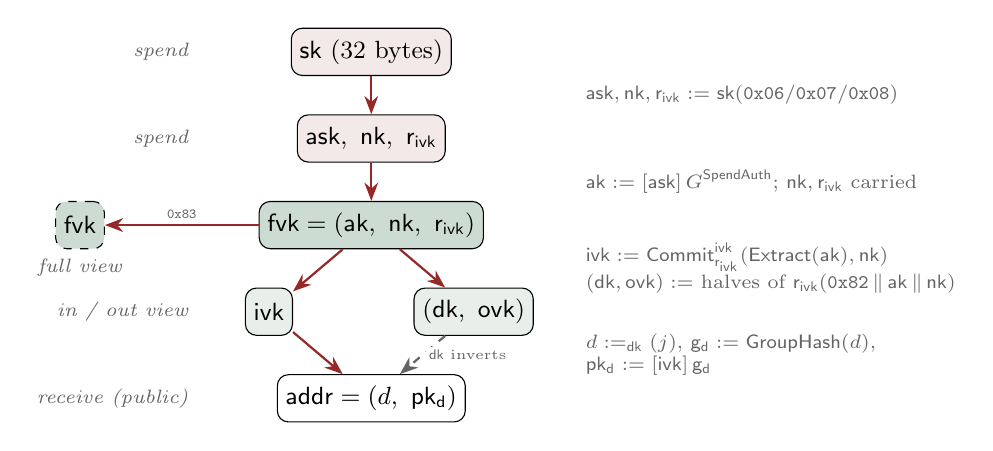
\begin{tikzpicture}[font=\small, x=1cm, y=1cm,
  k/.style={draw, rounded corners, inner sep=3pt, minimum height=6mm,
            anchor=center, fill=arb!10},
  kspend/.style={k, fill=arbred!10},
  kfull/.style={k, fill=arb!22},
  kpub/.style={k, fill=white},
  kint/.style={k, dashed, fill=arb!22},
  tier/.style={font=\scriptsize\itshape, text=arbdim, anchor=east},
  op/.style={font=\scriptsize, text=arbdim, anchor=west, align=left},
  elab/.style={font=\tiny, text=arbdim, inner sep=1pt, fill=white},
  ow/.style={-{Stealth}, thick, arbred},
  inv/.style={-{Stealth}, thick, arbdim, dashed}]
\node[kspend] (sk)    at (0,0)       {$\mathsf{sk}$ (32 bytes)};
\node[kspend] (mid)   at (0,-1.1)    {$\asksym,\ \nksym,\ \rivk$};
\node[kfull]  (fvk)   at (0,-2.2)    {$\fvk = (\aksym,\ \nksym,\ \rivk)$};
\node[kint]   (int)   at (-3.7,-2.2) {$\wbDint{\fvk}$};
\node[k]      (ivk)   at (-1.3,-3.3) {$\ivk$};
\node[k]      (dkovk) at (1.3,-3.3)  {$(\dk,\ \ovk)$};
\node[kpub]   (addr)  at (0,-4.4)    {$\mathsf{addr} = (d,\ \pkd)$};
\draw[ow] (sk)  -- (mid);
\draw[ow] (mid) -- (fvk);
\draw[ow] (fvk) -- (ivk);
\draw[ow] (fvk) -- (dkovk);
\draw[ow] (fvk) -- node[elab, above=1pt]{$\mathtt{0x83}$} (int);
\draw[ow] (ivk) -- (addr);
\draw[inv] (dkovk) -- node[elab, right=1pt]{$\dk$ inverts} (addr);
\node[op] at (2.6,-0.55)
  {$\asksym, \nksym, \rivk := \wbDprf{\mathsf{sk}}
   (\mathtt{0x06} / \mathtt{0x07} / \mathtt{0x08})$};
\node[op] at (2.6,-1.65)
  {$\aksym := [\asksym]\,G^{\mathsf{SpendAuth}}$; $\nksym, \rivk$ carried};
\node[op] at (2.6,-2.75)
  {$\ivk := \CommitIvk_{\rivk}(\Extract(\aksym), \nksym)$\\
   $(\dk, \ovk) :=$ halves of
   $\wbDprf{\rivk}(\mathtt{0x82}\,\|\,\aksym\,\|\,\nksym)$};
\node[op] at (2.6,-3.85)
  {$d := \wbDff_{\dk}(j)$, $\gd := \GroupHash(d)$,\\
   $\pkd := [\ivk]\,\gd$};
\node[tier] at (-2.2,0)    {spend};
\node[tier] at (-2.2,-1.1) {spend};
\node[tier, anchor=north] at (int.south) {full view};
\node[tier] at (-2.2,-3.3) {in / out view};
\node[tier] at (-2.2,-4.4) {receive (public)};
\end{tikzpicture}}

\begin{board}{BIP-32 becomes ZIP-32: one seed, two trees}{authorised}
\Write
\begin{enumerate}
  \item one seed: $32$--$252$ bytes, at least $256$ bits of entropy
  \item $(\mathsf{sk}_i, c_i) := \text{halves of }
    \wbDprf{c_{\mathrm{par}}}\bigl(\mathtt{0x81}\,\|\,
    \mathsf{sk}_{\mathrm{par}}\,\|\,i\bigr)$, \quad $i \ge 2^{31}$
  \item transparent:
    $m/44'/133'/\mathit{account}'/\mathit{change}/\mathit{index}$ ---
    two lowest levels non-hardened, xpub at the account
  \item Orchard: $m_{\mathsf{Orchard}}/32'/133'/\mathit{account}'$ ---
    hardened only, chain code discarded at the account, no change level
\end{enumerate}
\Say
\begin{itemize}
  \item One seed roots both trees, as one BIP-32 seed roots a Bitcoin
    wallet: one backup recovers every key.
  \item Orchard has no xpub mode (a public key deriving child public
    keys), so no Orchard extended full viewing key exists.
  \item No change level: a shielded change output is indistinguishable
    on chain from any other output, so a change subtree would separate
    nothing.
\end{itemize}
\end{board}

\begin{board}{Two scopes per account: external and internal}{authorised}
\Write
\begin{enumerate}
  \item $\wbDint{\rivk} := \mathrm{ToScalar}\bigl(\wbDprf{\rivk}(
    \mathtt{0x83}\,\|\,\aksym\,\|\,\nksym)\bigr)$
  \item $\wbDint{\fvk} := (\aksym,\ \nksym,\ \wbDint{\rivk})$
  \item same \asksym{} spends, same \nksym{} nullifies;
    \ivk, \dk, \ovk{} re-derived
  \item $\fvk \to \wbDint{\fvk}$; \quad $(\dk, \ivk) \to$ external scope
    only
\end{enumerate}
\Say
\begin{itemize}
  \item Only \rivk{} changes. The map $\mathrm{ToScalar}$ reduces the
    $512$-bit PRF output modulo the Pallas scalar-field order; an
    internal address does not decrypt under the external \ivk.
  \item A full viewing key sees both scopes. An external $(\dk, \ivk)$
    --- a payment processor --- sees the external scope only: neither
    the internal scope nor any \ovk{} follows from it.
  \item BIP-44 separates change by a path level on a public graph; here
    the separation is a second full viewing key, and the change output
    looks like any other output on chain.
\end{itemize}
\end{board}

\begin{board}{The internal scope: change and auto-shielding}{authorised}
\Write
\begin{enumerate}
  \item internal addresses $\leftarrow$ change, auto-shielded funds
  \item shielding $=$ moving transparent funds into the pool
    (automatic, to an internal address)
  \item Alice's change: $0.4999$ ZEC $\to$ internal address, index $0$
\end{enumerate}
\Say
\begin{itemize}
  \item What BIP-44 puts in the path sits here in the key.
  \item The deployed wallet library sends change to the internal address
    at index $0$.
  \item A Bitcoin change output sits on the change branch of a public
    graph; here the change output is indistinguishable from any other,
    and only the internal scope's keys find it.
\end{itemize}
\end{board}

\begin{board}{The ladder: one secret, graded capabilities}
  {authorised / not twice}
\begin{center}
\resizebox{!}{0.6\textheight}{\wbDLadderFig}
\end{center}
\newpage
\Write
\begin{enumerate}
  \item $\asksym, \nksym, \rivk := \wbDprf{\mathsf{sk}}
    (\mathtt{0x06} / \mathtt{0x07} / \mathtt{0x08})$
  \item $\aksym := [\asksym]\,G^{\mathsf{SpendAuth}}$; \ $\nksym, \rivk$
    carried
  \item $\ivk := \CommitIvk_{\rivk}(\Extract(\aksym), \nksym)$
  \item $(\dk, \ovk) :=$ halves of
    $\wbDprf{\rivk}(\mathtt{0x82}\,\|\,\aksym\,\|\,\nksym)$
  \item $d := \wbDff_{\dk}(j)$, \ $\gd := \GroupHash(d)$, \
    $\pkd := [\ivk]\,\gd$
\end{enumerate}
\Say
\begin{itemize}
  \item Red arrows are one-way: a rung is handed down without the powers
    above it.
  \item Bitcoin's BIP-32 has two rungs, xprv and xpub, and the public
    ledger supplies the rest; here every rung between is a separate
    secret, and only the address is public.
  \item The pair $(\dk, \ovk)$ comes from \fvk{} by a PRF, not from
    \ivk: the two branches leaving \fvk{} are siblings.
  \item The circuit re-walks $\fvk \to \ivk \to \pkd$ (A7) with \gd{} as
    a witness; the step $j \to d \to \gd$ is never checked in the
    circuit (the dashed grey edge).
\end{itemize}
\end{board}

\begin{board}{What holds the rungs apart}{authorised / not twice}
\begin{center}
\begin{tabular}{@{}lll@{}}
\toprule
step & operation & why it is one-way \\
\midrule
$\mathsf{sk} \to (\asksym, \nksym, \rivk)$ &
  $\wbDprf{\mathsf{sk}}(\mathtt{0x06}/\mathtt{0x07}/\mathtt{0x08})$ &
  PRF (BLAKE2b) \\
$\asksym \to \aksym$ & $[\asksym]\,G^{\mathsf{SpendAuth}}$ &
  discrete log on Pallas \\
$\fvk \to \ivk$ & $\CommitIvk_{\rivk}(\Extract(\aksym), \nksym)$ &
  hiding under \rivk \\
$\fvk \to (\dk, \ovk)$ &
  halves of $\wbDprf{\rivk}(\mathtt{0x82}\,\|\,\aksym\,\|\,\nksym)$ &
  PRF \\
$\fvk \to \wbDint{\fvk}$ &
  $\wbDprf{\rivk}(\mathtt{0x83}\,\|\,\aksym\,\|\,\nksym)$ & PRF \\
$\ivk \to \pkd$ & $[\ivk]\,\gd$ & discrete log on Pallas \\
$j \to d$ & $\wbDff_{\dk}(j)$ & \emph{not} one-way: \dk{} inverts it \\
\bottomrule
\end{tabular}
\end{center}
\newpage
\Write
\begin{enumerate}
  \item the scalar \ivk: a commitment, not a hash --- binds \emph{and}
    hides $(\aksym, \nksym)$
  \item one \rivk{} keys both $\CommitIvk$ and the $\mathtt{0x82}$ PRF
    $\Rightarrow$ joint assumption once \dk{} or \ovk{} is exposed
  \item a separate \nksym: spent status without spend authority
\end{enumerate}
\Say
\begin{itemize}
  \item Three kinds of wall: a PRF (BLAKE2b) at the top and at the
    $\mathtt{0x82}$ and $\mathtt{0x83}$ splits; a discrete logarithm on
    Pallas at $\asksym \to \aksym$ and $\ivk \to \pkd$; a hiding
    commitment at $\fvk \to \ivk$.
  \item An \ivk{} holder learns neither \aksym{} nor \nksym. The viewing
    key holds \nksym, never \asksym.
  \item The last row is deliberately not one-way: the \dk{} holder maps
    any of its addresses back to an index. Bitcoin has one wall, xprv to
    xpub; the rest of its ladder is public.
\end{itemize}
\end{board}

\begin{board}{Graded capabilities: spend, full view, spent status}
  {authorised / not twice}
\begin{center}\small
\begin{tabular}{@{}p{18mm}p{30mm}p{48mm}p{37mm}@{}}
\toprule
capability & holds & can & cannot \tabularnewline
\midrule
spend & \asksym{} (from $\mathsf{sk}$) &
  \raggedright authorise spends, both scopes & --- \tabularnewline
\raggedright full view & $\fvk = (\aksym, \nksym, \rivk)$ &
  \raggedright everything below, both scopes; every address and its
  index &
  \raggedright spend: \asksym{} is a discrete log away \tabularnewline
\raggedright spent status & \nksym{} (inside \fvk) &
  \raggedright the nullifier of a note it holds &
  \raggedright spend; find notes (needs \ivk) \tabularnewline
\bottomrule
\end{tabular}
\end{center}
\Write
\begin{enumerate}
  \item Bitcoin: only the spend row is secret (xprv)
\end{enumerate}
\Say
\begin{itemize}
  \item Each row holds strictly less than the one above. A full viewing
    key sees everything and moves nothing: \asksym{} is a discrete
    logarithm away from \aksym.
  \item Full view and spent status are what Bitcoin's public ledger
    shows to everyone.
\end{itemize}
\end{board}

\begin{board}{Graded capabilities: incoming, outgoing, receive}{exists}
\begin{center}\small
\begin{tabular}{@{}p{18mm}p{30mm}p{48mm}p{37mm}@{}}
\toprule
capability & holds & can & cannot \tabularnewline
\midrule
\raggedright incoming view & $(\dk, \ivk)$ &
  \raggedright detect and decrypt incoming; derive all $2^{88}$
  addresses and invert them to indices &
  \raggedright nullifiers, so spent status; outgoing; the internal
  scope \tabularnewline
\raggedright outgoing view & \ovk &
  \raggedright open $C_{\mathrm{out}}$ of what this account and scope
  sent (a sender may set $\ovk = \bot$: then no \ovk{} opens it) &
  \raggedright incoming; the internal \ovk \tabularnewline
receive & $(d, \pkd)$ & be paid &
  \raggedright anything else --- the only public item \tabularnewline
\bottomrule
\end{tabular}
\end{center}
\Write
\begin{enumerate}
  \item every row but the last is a distinct secret
\end{enumerate}
\newpage
\Say
\begin{itemize}
  \item Bitcoin's ledger collapses everything between xprv and the
    address into what anyone can read.
  \item The incoming view sees arrivals, not departures: no nullifiers,
    so no spent status, no outgoing view, no internal scope.
  \item The outgoing view may open nothing: a sender may set
    $\ovk = \bot$.
  \item The address is the only public item: it lets one be paid and
    does nothing else.
\end{itemize}
\end{board}

\begin{board}{Viewing keys: xpub is the bridge, not the analogue}
  {exists / not twice}
\Write
\begin{enumerate}
  \item xpub $=$ watch-only: enumerates addresses; the public ledger
    supplies incoming, outgoing, spent status --- to anyone
  \item $(\dk, \ivk)$ $=$ watch-only for incoming: enumerates \emph{and}
    decrypts
  \item three differences: (1) nothing visible without the key;
    (2) spent status $=$ \nksym; (3) outgoing $=$ \ovk
  \item ``viewing'' $=$ a capability, not publicity
\end{enumerate}
\Say
\begin{itemize}
  \item Nothing is visible without the key because the outputs are
    ciphertext. The key \nksym{} computes the nullifiers matched against
    the chain's set; the key \ovk{} opens $C_{\mathrm{out}}$. The xpub
    gets both free only because Bitcoin's ledger is public.
  \item Every viewing key is secret material disclosed deliberately ---
    to an auditor, a processor --- and validation needs none of them.
\end{itemize}
\end{board}

\begin{board}{Diversified addresses: one key, $2^{88}$ addresses}{exists}
\Write
\begin{enumerate}
  \item $d := \wbDff_{\dk}(j)$
  \item $\gd := \wbDgh$
  \item $\pkd := [\ivk]\,\gd$, \quad $\mathsf{addr} := (d,\ \pkd)$
  \item $2^{88} \approx 3.1 \times 10^{26}$ addresses per key;
    raw receiver $11 + 32 = 43$ bytes
  \item random $88$-bit draws collide near $2^{44}$; FF1 never collides,
    and \dk{} inverts it
\end{enumerate}
\Say
\begin{itemize}
  \item Every index works: $\GroupHash$ is total (a fixed fallback
    covers the identity), so there is no rejection loop. All addresses
    are spent by one \asksym{} and found by one \ivk, at no extra
    scanning cost.
  \item A keyed permutation, not a counter and not a hash: the wallet
    stores nothing per address.
  \item Wallet-side only, never in the circuit: the circuit takes \gd{}
    as a witness (the ladder board) and never sees $j$, so AES is fine
    here.
\end{itemize}
\end{board}

\begin{board}{Unlinkable, even to the payer}{exists}
\Write
\begin{enumerate}
  \item $(d, \pkd)$ and $(d', \pkd')$: \ $\pkd = [\ivk]\,\gd$,
    \ $\pkd' = [\ivk]\,\gd'$ \ --- same \ivk?
  \item deciding it $=$ DDH on Pallas, $\GroupHash$ a random oracle
  \item only $(\dk, \ivk)$ can check: re-derive at the decrypted index
  \item never a chosen-diversifier oracle
\end{enumerate}
\Say
\begin{itemize}
  \item Given two addresses of different owners and a third derived from
    one of them, no one can tell which. Alice, who paid one of Bob's
    addresses, learns nothing about the other.
  \item A chosen-diversifier oracle --- an address for an attacker's $d$
    under your \ivk{} --- breaks unlinkability for every address of that
    \ivk.
  \item Under one xpub, addresses link on the public graph once spent
    together (Part~A), and a leaked xpub links all beneath it, spent or
    not. Here an address reveals only itself.
\end{itemize}
\end{board}

\begin{board}{Unified addresses (ZIP-316): one string, several receivers}
  {exists}
\Write
\begin{enumerate}
  \item typecodes: $\mathtt{0x00}$ P2PKH, $\mathtt{0x01}$ P2SH,
    $\mathtt{0x02}$ Sapling, $\mathtt{0x03}$ Orchard --- at most one
    each, at least one shielded
  \item ascending typecode $\to$ F4Jumble (whole payload, HRP included)
    $\to$ Bech32m
  \item sender: Orchard $>$ Sapling $>$ transparent; may refuse a type,
    never reorder
  \item Orchard receiver $\to$ the Ironwood pool
\end{enumerate}
\Say
\begin{itemize}
  \item F4Jumble is an unkeyed four-round Feistel permutation of the
    whole payload, so a substituted receiver changes the whole string,
    not one region of it.
  \item An Orchard receiver names the protocol, not a pool; all new
    value enters the Ironwood pool, so a payment to it lands in the
    Ironwood tree.
  \item The same container with viewing-key items is a unified full or
    incoming viewing key.
  \item One Bitcoin address encodes one script type; here one address
    lets the sender's wallet choose the pool.
\end{itemize}
\end{board}

\begin{board}{Bob's address in the example}{exists}
\Write
\begin{enumerate}
  \item $\mathsf{addr}_B = (d_B,\ \pkd)$, $43$ bytes
  \item $\gd := \GroupHash^{\Pallas}(\mathtt{z.cash:Orchard\text{-}gd},\
    d_B)$, \quad $\epk := [\esk]\,\gd$
  \item $\mathbf{n} := (\mathsf{addr}_B,\ 1.5\ \text{ZEC},\ \rho,\ \psi,\
    \rcm)$
  \item on chain: inside \cmsym, inside $C_{\mathrm{enc}}$, as \epk{}
    under a fresh \esk; lead byte $\mathtt{0x03}$
  \item change $0.4999$ ZEC $\to$ Alice's internal address, index $0$
\end{enumerate}
\Say
\begin{itemize}
  \item Bob hands Alice a unified address; her wallet takes its Orchard
    receiver and learns nothing else: no \ivk, \nksym{} or \aksym, no
    index $j$, no link to Bob's other addresses.
  \item The note is minted in the Ironwood tree; Bob's one \ivk{}
    trial-decrypts both pools. No address of Alice's appears either.
  \item Bitcoin displays the script beside the amount; here neither
    appears in the clear.
\end{itemize}
\newpage
\Ask
Which key does an accountant need to audit a company's incoming
\emph{and} outgoing shielded payments --- and what can they not do with
it?
\Answer
\begin{itemize}
  \item One unified full viewing key per account. Inside it, \fvk{}
    yields \ivk{} (incoming), \nksym{} (which of those notes are spent)
    and \ovk{} (outgoing) --- for the external scope and, through the
    $\mathtt{0x83}$ step, the internal one, so change is covered too.
  \item Not spend: \asksym{} is a discrete logarithm away from \aksym.
    Not wander into a sibling account: only hardened derivation exists,
    and no Orchard extended full viewing key.
  \item Not read what was sent under some other \ovk, or under none
    ($\ovk = \bot$); nor anything received by an account they were not
    given.
\end{itemize}
\end{board}

%% ---- 05-statement.tex
%% ---- Part E --- The Action statement: screen version
\newcommand{\wbEcv}{\ensuremath{\cvsym^{\mathsf{net}}}}
\newcommand{\wbEnf}{\ensuremath{\nfsym_{\mathrm{old}}}}
\newcommand{\wbEanc}{\ensuremath{\mathsf{anchor}}}
\newcommand{\wbEold}[1]{\ensuremath{#1_{\mathrm{old}}}}
\newcommand{\wbEnew}[1]{\ensuremath{#1_{\mathrm{new}}}}
\newcommand{\wbEcenc}{\ensuremath{C_{\mathrm{enc}}}}
\newcommand{\wbEcout}{\ensuremath{C_{\mathrm{out}}}}
\newcommand{\wbEflag}[1]{\ensuremath{\mathsf{#1}}}
\newcommand{\wbEPoseidon}{\ensuremath{\mathsf{Poseidon}}}
\newcommand{\wbEgsa}{\ensuremath{G^{\mathsf{SpendAuth}}}}
\newcommand{\wbEgnf}{\ensuremath{G^{\mathsf{nf}}}}
% \wbEActionBox[field]: one Action inside its bundle; field in
% {none, anchor, nf, cv, rk, cmx, proof} is drawn highlighted.
\newcommand{\wbEActionBox}[1][none]{%
  \tikzset{wbEhlnone/.style={}, wbEhlanchor/.style={}, wbEhlnf/.style={},
    wbEhlcv/.style={}, wbEhlrk/.style={}, wbEhlcmx/.style={},
    wbEhlproof/.style={},
    wbEhl#1/.style={draw=arbred, very thick, fill=arbred!15}}%
  \begin{tikzpicture}[font=\scriptsize, x=1cm, y=1cm,
    ebox/.style={draw=black!60, fill=white, rounded corners=2pt,
      inner sep=2.5pt, align=center},
    elab/.style={inner sep=2pt, text=black!60}]
  % the bundle; a second Action behind the first
  \draw[draw=black!50, dashed, rounded corners=3pt]
    (-2.45,-2.45) rectangle (4.75,2.5);
  \node[elab, anchor=north west, text=black!70, font=\scriptsize\bfseries]
    at (-2.45,2.5) {bundle};
  \draw[draw=arb!40, rounded corners=3pt] (-2.0,-2.1) rectangle (2.4,2.1);
  \node[elab, anchor=south east, text=arb!60] at (2.4,2.1) {$\times\,n$};
  \node[draw=arb, thick, fill=white, rounded corners=3pt,
    minimum width=4.4cm, minimum height=3.9cm] (act) at (0,0) {};
  \node[anchor=north west, font=\scriptsize\bfseries, text=arb,
    inner sep=2pt] at (act.north west) {Action};
  \node[draw=arb!60, fill=arb!8, rounded corners=2pt, inner sep=3pt,
    align=center, anchor=north, text width=3.8cm] (wit) at (0,1.62)
    {\textbf{witness} --- never published\\
     old note, new note\\
     Merkle path $+$ position\\
     $\aksym, \nksym, \rivk, \ivk$; $\alpha$, $\rcv$};
  \node[elab, anchor=west] at (-2.15,-0.12) {public, per Action};
  \node[ebox, wbEhlcv, anchor=west] (cv) at (-2.05,-0.58) {$\wbEcv$};
  \node[ebox, wbEhlnf, right=1.2mm of cv] (nf) {$\wbEnf$};
  \node[ebox, wbEhlrk, right=1.2mm of nf] (rk) {$\rksym$};
  \node[ebox, wbEhlcmx, right=1.2mm of rk] (cmx) {$\cmx$};
  \node[ebox, draw=black!40, dashed] (ct) at (0,-1.15)
    {$\epk,\ \wbEcenc,\ \wbEcout$};
  \node[elab, align=center, font=\tiny, text=black!60] at (0,-1.66)
    {delivery ciphertexts --- no in-circuit check;\\
     opened only with $\ivk$/$\ovk$ (\emph{Delivery})};
  % bundle-level fields
  \node[ebox, wbEhlanchor, anchor=west] (anc) at (2.45,1.65) {$\wbEanc$};
  \node[ebox, anchor=west] (flg) at (2.45,1.0) {flags};
  \node[ebox, anchor=west] (vb)  at (2.45,0.35) {$v_{\mathrm{balance}}$};
  \node[ebox, wbEhlproof, anchor=west] (prf) at (2.45,-0.3) {proof};
  \node[ebox, anchor=west] (sas) at (2.45,-0.95) {SpendAuthSigs};
  \node[ebox, anchor=west] (bsg) at (2.45,-1.6) {binding sig};
  \end{tikzpicture}}
% Figure in the left column (fraction #1 of the text width) with #3 under
% it (the Ask, or empty); the board's text (#4) beside it, in \small.
\newcommand{\wbEbeside}[4][0.35]{%
  \noindent\begin{minipage}[c]{#1\textwidth}
    \noindent\resizebox{\linewidth}{!}{#2}\par\small #3\end{minipage}\hfill
  \begin{minipage}[c]{\dimexpr0.97\textwidth-#1\textwidth\relax}\small
    \abovedisplayskip=4pt \belowdisplayskip=4pt
    \abovedisplayshortskip=4pt \belowdisplayshortskip=4pt
    #4\end{minipage}\par}
% Three-column table; \wbErow ends rows so ragged cells work without array.
\newenvironment{wbEtable}[1]{\par\smallskip\noindent\small
  \setlength{\tabcolsep}{3pt}\renewcommand{\arraystretch}{1.05}%
  \begin{tabular}{@{}#1@{}}\toprule}{\bottomrule\end{tabular}\par}
\newcommand{\wbErr}{\raggedright}
\newcommand{\wbErow}[3]{#1 & \wbErr #2 & \wbErr #3 \tabularnewline}

\section{Part E --- The Action statement}

\begin{board}{Anatomy of an Action}{all four}
\wbEbeside[0.45]{\wbEActionBox}{}{%
\Write
\begin{itemize}
  \item one Action $=$ one old note spent $+$ one new note created
  \item witness (never published): old note, new note, path $+$
    position, $\aksym, \nksym, \rivk, \ivk$, $\alpha$, $\rcv$
  \item rim, per Action: $\wbEcv$, $\wbEnf$, $\rksym$, $\cmx$ --- the four
    the proof binds
  \item dashed: $\epk$, $\wbEcenc$, $\wbEcout$ --- ciphertexts, read by no
    clause
\end{itemize}}
\Say
\begin{itemize}
  \item The shape is fixed: an Action never shows which it ``really'' is.
  \item Bitcoin: an input names its coin and shows its script; an output
    shows its amount and its script. Here every field is a commitment, a
    serial number, a disguised key, or a ciphertext.
\end{itemize}
\end{board}

\begin{board}{The bundle around it}{all four}
\begin{wbEtable}{p{24mm}p{58mm}p{58mm}}
\wbErow{\textbf{per bundle}}{\textbf{once}}{\textbf{role}}
\midrule
\wbErow{$\wbEanc$}{one root, shared by every Action}{the tree the spends
  prove membership in}
\wbErow{flags}{$\wbEflag{enableSpends}$, $\wbEflag{enableOutputs}$,
  $\wbEflag{enableCrossAddress}$}{consensus gates (A8--A10)}
\wbErow{$v_{\mathrm{balance}}$}{signed, cleartext}{net value leaving the
  pool}
\wbErow{proof}{one aggregate Halo 2 proof}{covers all $n$ Actions at once}
\wbErow{binding sig}{one signature}{proves the values balance}
\addlinespace[4pt]
\wbErow{per Action}{SpendAuthSig under $\rksym$}{the owner authorised
  this spend}
\end{wbEtable}
\Write
\begin{itemize}
  \item one Action $= 820$ public bytes, $660$ of them ciphertext
  \item Alice: $2$ Actions, one $7264$-byte proof
  \item node checks: proof, anchor, nullifier set, two signatures ---
    never a note
\end{itemize}
\end{board}

\begin{board}{Why a spend and an output are fused}{all four}
\Write
\[
n_{\mathrm{act}}(s, o) = \max\bigl(\max(s, o),\, 2\bigr)
\qquad\text{Alice: } s = 1,\ o = 2 \;\Rightarrow\; n_{\mathrm{act}} = 2
\]
\begin{itemize}
  \item spend list and output list each padded to $n_{\mathrm{act}}$;
    floor $2$
  \item Alice: $1$ spend, $2$ outputs (Bob, change) $\Rightarrow$ one
    dummy spend
\end{itemize}
\Say
\begin{itemize}
  \item A Bitcoin transaction shows its true input and output counts.
    Here the count is $n_{\mathrm{act}}$, and the fee is computed from
    that public count (\emph{The transaction and the turnstile}).
  \item Every Action looks like every other: one spend slot, one output
    slot, whatever the payment needed.
  \item This count and the shuffle are the Ironwood component's
    (cross-address enabled). A sealed Orchard-pool bundle pads to
    $s + o$ and pairs each spend with an output to the spent note's own
    receiver.
\end{itemize}
\end{board}

\begin{board}{Dummies and the shuffle}{all four}
\Write
\begin{itemize}[leftmargin=1em]
  \item dummy spend: value $0$, fresh random spending key,
    $\rho = \Extract(\text{random Pallas point})$; still publishes a
    nullifier
  \item dummy output: value $0$, fresh random address,
    $\rho := \wbEnf$ like any output's
  \item shuffle spends and outputs \emph{independently}, then zip
  \item Alice: spend side $\{2\text{ ZEC note}, \text{dummy}\}$; output
    side $\{\text{Bob}, \text{change}\}$
\end{itemize}
\Say
\begin{itemize}
  \item Which spend shares an Action with which output is the shuffle's
    choice.
  \item Bitcoin: an input is an input and an output is an output. Here a
    dummy spend looks exactly like a real one and, like a real one,
    publishes a nullifier the pool records.
\end{itemize}
\end{board}

\begin{board}{The statement, in the validator's language}{all four}
\Write
\begin{itemize}
  \item \emph{``Some leaf under this anchor is a note I own; this is its
    serial number; this commitment hides its value change; this signing
    key is a fresh disguise of the owner's --- and I have shown you
    neither the leaf, the note, nor the owner's key.''}
  \item public: $\wbEanc$, $\wbEcv$, $\wbEnf$, $\rksym$, $\cmx$, three
    flags --- $8$ names, $10$ field elements
  \item witness: both notes, path $+$ position, $\aksym$, $\nksym$,
    $\rivk$, $\ivk$, $\alpha$, $\rcv$
  \item relation: ten clauses A1--A10; one verifying key, selected by
    branch; a proof of nine fails
\end{itemize}
\Say
\begin{itemize}
  \item The two Pallas points enter by their coordinates. Here $\wbEcv$
    and $\wbEnf$ are the data model's $\cvsym$ and $\nfsym$, marked
    \emph{net} (this Action's value change) and \emph{old} (the note
    spent).
  \item A proof of nine clauses is a proof for a different circuit, and
    it fails.
  \item Bitcoin's validator runs \emph{your} script. This validator runs
    one verifier keyed to one fixed circuit; the transaction supplies
    inputs, never logic.
\end{itemize}
\end{board}

\begin{board}{The ten clauses, ordered by the four checks}{all four}
\begin{wbEtable}{p{50mm}p{12mm}p{78mm}}
\wbErow{\textbf{Bitcoin's check}}{\textbf{clause}}{\textbf{what the proof
  establishes}}
\midrule
\wbErow{coin exists (UTXO lookup)}{A3}{a Merkle path from
  $\wbEold{\cmsym}$ to the anchor}
\wbErow{not spent twice (entry deleted)}{A5}{$\wbEnf$ is this note's
  serial, keyed by $\nksym$}
\wbErow{conserved ($\sum\mathrm{in} \ge \sum\mathrm{out}$)}{A4}{$\wbEcv$
  hides $\wbEold{v} - \wbEnew{v}$, both below $2^{64}$}
\wbErow{authorised (script $+$ signature)}{A6, A7}{$\rksym$ disguises
  $\aksym$; $\aksym, \nksym$ sit behind the address}
\addlinespace[4pt]
\wbErow{well-formed}{A1, A2}{both commitments open to notes;
  $\wbEnew{\rho} = \wbEnf$}
\wbErow{gated}{A8, A9}{spends and outputs switched on by the flags}
\wbErow{sealed}{A10}{cross-address transfers switched off, or not}
\end{wbEtable}
\Write
\begin{itemize}
  \item $4$ Bitcoin checks $\to$ $7$ clauses (A1--A7); $3$ consensus
    gates (A8--A10)
  \item stays with the node: ``has this serial been seen?''
\end{itemize}
\end{board}

\begin{board}{Alice's two Actions against the ten clauses}{all four}
\begin{wbEtable}{p{14mm}p{63mm}p{63mm}}
\wbErow{\textbf{clause}}{\textbf{Action 1: $2$ ZEC $\to$ Bob $1.5$}}
  {\textbf{Action 2: dummy $\to$ change $0.4999$}}
\midrule
\wbErow{A1}{Alice's $2$ ZEC note opens $\wbEold{\cmsym}$}{a zero-value
  dummy opens $\wbEold{\cmsym}$}
\wbErow{A2}{Bob's note; $\wbEnew{\rho} := \nfsym$ of Alice's note}{change
  note; $\wbEnew{\rho} := \nfsym$ of the dummy}
\wbErow{A3}{a $32$-sibling path to the Ironwood anchor}{gated off:
  $\wbEold{v} = 0$}
\wbErow{A4}{$\wbEcv$ commits to $+0.5$ ZEC}{$\wbEcv$ commits to
  $-0.4999$ ZEC}
\wbErow{A5}{$\nfsym$ of Alice's note, under her $\nksym$}{$\nfsym$ of the
  dummy, under its random $\nksym$}
\wbErow{A6}{$\rksym = \aksym + [\alpha]\,\wbEgsa$, Alice's $\aksym$}{the
  same, the dummy's $\aksym$}
\wbErow{A7}{Alice's $\aksym, \nksym$ sit behind her address}{the dummy's
  key, behind its address}
\wbErow{A8, A9}{both flags set: both products vanish}{the same}
\wbErow{A10}{$\delta = 0$ (Ironwood): nothing constrained}{the same}
\end{wbEtable}
\Write
\[
+0.5 - 0.4999 = +0.0001\text{ ZEC} = 10\,000\text{ zatoshi} =
\text{fee} = v_{\mathrm{balance}}
\]
\end{board}

\begin{board}{What Alice's public fields carry}{all four}
\begin{wbEtable}{p{14mm}p{60mm}p{67mm}}
\wbErow{\textbf{field}}{\textbf{Action 1}}{\textbf{Action 2}}
\midrule
\wbErow{$\wbEcv$}{$+0.5$ ZEC under a fresh $\rcv$}{$-0.4999$ ZEC under a
  fresh $\rcv$}
\wbErow{$\wbEnf$}{Alice's note's serial: the note is retired}{the
  dummy's serial, recorded all the same}
\wbErow{$\rksym$}{a fresh disguise of Alice's $\aksym$}{a fresh disguise
  of the dummy's $\aksym$}
\wbErow{$\cmx$}{Bob's $1.5$ ZEC note}{Alice's $0.4999$ ZEC change note,
  at her internal address}
\wbErow{$\epk, \wbEcenc$}{to Bob's $\pkd$; opened with his $\ivk$}{to
  Alice's internal $\pkd$; found with $\ivk^{\mathsf{int}}$}
\wbErow{$\wbEcout$}{under Alice's $\ovk$: she can re-read it}{no $\ovk$
  for change (wallet default): unrecoverable}
\addlinespace[4pt]
bundle & \multicolumn{2}{p{\dimexpr127mm+6pt\relax}@{}}{\wbErr one
  Ironwood anchor; flags $(1, 1, 1)$; $v_{\mathrm{balance}} = +10\,000$
  zatoshi; one proof; two SpendAuthSigs; one binding signature}
  \tabularnewline
\end{wbEtable}
\Write
\begin{itemize}
  \item which is ``Action 1'' on the wire: the shuffle decides
  \item $2$ nullifiers, $2$ commitments: every two-Action bundle
\end{itemize}
\end{board}

\begin{board}{Coin exists --- A3, the path to the anchor}{exists}
\wbEbeside{\wbEActionBox[anchor]}{\Ask Which of the four checks?}{%
\Write
\begin{itemize}
  \item fold $\Extract(\wbEold{\cmsym})$ up $32$ witnessed siblings to
    $\mathsf{root}$
  \item $\wbEold{v} \cdot (\mathsf{root} - \wbEanc) = 0$
  \item witness: siblings, position bits; public: $\wbEanc$, one per
    bundle
\end{itemize}
\Say
\begin{itemize}
  \item Bitcoin looks the coin up in the UTXO set, and so names it. This
    clause says only ``some leaf under this anchor'': the candidate set
    is the Ironwood tree under the anchor.
  \item A zero-value dummy skips the check by arithmetic, not by a flag.
\end{itemize}}
\Answer
Coin exists.
\end{board}

\begin{board}{No double spend --- A5, the nullifier}{not twice}
\wbEbeside{\wbEActionBox[nf]}{\Ask Which check?}{%
\Write
\begin{gather*}
\wbEnf = \Extract\bigl([\,\wbEPoseidon_{\nksym}(\wbEold{\rho}) +
  \wbEold{\psi}\,]\,\wbEgnf + \wbEold{\cmsym}\bigr)
\end{gather*}
\begin{itemize}
  \item three lines: membership (A3), serial (A5), balance (A4)
\end{itemize}
\Say
\begin{itemize}
  \item Bitcoin deletes the entry; here an unlinkable serial is added.
  \item Clause A5 binds the published serial to the spent note under the
    witnessed $\nksym$; otherwise a spender could invent a fresh serial
    per spend and the set would never repeat.
  \item ``Seen before?'' is global history: the node checks the set, the
    proof cannot.
\end{itemize}}
\Answer
Not spent twice.
\end{board}

\begin{board}{Authorised --- the linkage problem first}{authorised}
\Write
\begin{gather*}
\ivk = \CommitIvk_{\rivk}\bigl(\Extract(\aksym), \nksym\bigr), \qquad
\pkd = [\ivk]\,\gd \quad\text{for every } d
\end{gather*}
\begin{itemize}
  \item one $\aksym$ per wallet, not per coin
  \item publish $\aksym$ $+$ signature $\Rightarrow$ every spend, from
    every address, linked
  \item needed: a fresh key per spend that still proves the same secret
\end{itemize}
\Say
\begin{itemize}
  \item Every diversified address shares $\aksym$ through $\ivk$
    (\emph{Keys and addresses}).
  \item Bitcoin's version of this is address reuse, and it is optional.
    Here it would be structural.
\end{itemize}
\end{board}

\begin{board}{Authorised --- A6, a disguised key}{authorised}
\wbEbeside{\wbEActionBox[rk]}{\Ask Which check?}{%
\Write
\[
\rksym = \aksym + [\alpha]\,\wbEgsa, \qquad \rsk = \asksym + \alpha
\]
\begin{itemize}
  \item circuit checks the shift; node checks a signature under $\rksym$
  \item uniform $\alpha$ $\Rightarrow$ uniform $\rksym$, whatever
    $\aksym$
\end{itemize}
\Say
\begin{itemize}
  \item Clause A6: the published key is $\aksym$ shifted by a fresh,
    secret $\alpha$.
  \item Bitcoin bridge: Schnorr with a per-spend tweak --- a
    non-hardened BIP-32 child whose tweak is uniform and never
    published.
\end{itemize}}
\Answer
Authorised.
\end{board}

\begin{board}{Authorised --- A7, one identity behind the address}{authorised}
\Write
\begin{gather*}
\ivk = \CommitIvk_{\rivk}\bigl(\Extract(\aksym), \nksym\bigr), \qquad
\wbEold{\pkd} = [\ivk]\,\wbEold{\gd}
\end{gather*}
\begin{itemize}
  \item one identity: signs (A6), nullifies (A5), is paid (A7)
  \item circuit: the key is the owner's; signature under $\rksym$: the
    spender holds it
\end{itemize}
\Say
\begin{itemize}
  \item Clause A6 alone proves a disguise of some $\aksym$; clause A7
    ties that $\aksym$, and the $\nksym$ of A5, to the spent note's
    address by the ladder of \emph{Keys and addresses}.
  \item Bitcoin: a P2PKH address \emph{is} the key's hash, so ``this key
    matches this coin'' is one hash comparison in the clear. Here the
    address is a commitment to the key, and the match is proved.
\end{itemize}
\end{board}

\begin{board}{Well-formed --- A1 and A2, both notes really are
  notes}{well-formed}
\Write
\begin{gather*}
\wbEold{\cmsym} = \NoteCommit_{\wbEold{\rcm}}(\mathbf{n}_{\mathrm{old}}),
\qquad
\Extract\bigl(\NoteCommit_{\wbEnew{\rcm}}(\mathbf{n}_{\mathrm{new}})\bigr)
= \cmx, \\
\text{with } \wbEnew{\rho} := \wbEnf .
\end{gather*}
\begin{itemize}
  \item note $=$ address, value, $\rho$, $\psi$; commitment binding
    $\Rightarrow$ one leaf, one note
  \item chain stores only $\cmx$
\end{itemize}
\Say
\begin{itemize}
  \item A Bitcoin output is plaintext: well-formed means it parses. Here
    the note is hidden, so ``this commitment opens to a note'' must be
    proved.
  \item The chain $\wbEnew{\rho} := \wbEnf$ is enforced here: accepted
    seeds are unique within the pool, and two notes cannot share a
    nullifier.
\end{itemize}
\end{board}

\begin{board}{Conserved --- A4, the value commitment}{conserved}
\wbEbeside{\wbEActionBox[cv]}{\Ask Which check?}{%
\Write
\begin{gather*}
\wbEcv = [\wbEold{v} - \wbEnew{v}]\,V + [\rcv]\,R, \\
\wbEold{v}, \wbEnew{v} \in [0, 2^{64}),\quad \text{sign} \in \{-1, +1\}
\end{gather*}
\begin{itemize}
  \item group order $\approx 2^{254}$: a value near the order is a small
    negative one
\end{itemize}
\Say
\begin{itemize}
  \item Bitcoin checks $\sum\mathrm{in} \ge \sum\mathrm{out}$ on amounts
    it can read; here they are hidden. Clause A4 commits to this
    Action's value \emph{change} under a fresh trapdoor $\rcv$; the
    bundle sums these (\emph{Balance and authority}).
  \item Unbounded, the books would ``balance'' while minting.
  \item Elements' range proof exists for the same reason; here it lives
    inside the Action proof, with the opening.
\end{itemize}}
\Answer
Conserved.
\end{board}

\begin{board}{Gated --- A8 and A9, the flags}{gated}
\Write
\begin{gather*}
\wbEold{v} \cdot (1 - \wbEflag{enableSpends}) = 0, \qquad
\wbEnew{v} \cdot (1 - \wbEflag{enableOutputs}) = 0
\end{gather*}
\begin{itemize}
  \item flag clear $\Rightarrow$ only value $0$ passes
  \item coinbase: $\wbEflag{enableSpends} = 0$; Alice: both flags set
\end{itemize}
\Say
\begin{itemize}
  \item Bitcoin's coinbase has one null input by format. Here the same
    rule is arithmetic on a hidden value --- the only way to gate what
    the node cannot read.
  \item The flags are bundle-level bits the node supplies as public
    inputs; the circuit only multiplies. A cleared
    $\wbEflag{enableSpends}$ admits dummies and nothing else.
  \item A coinbase must clear $\wbEflag{enableSpends}$: its Actions spend
    dummies and create the block's shielded reward.
\end{itemize}
\end{board}

\begin{board}{Sealed --- A10, the cross-address gate}{sealed}
\Write
\begin{gather*}
\delta \cdot \bigl(x(\wbEold{\gd}) - x(\wbEnew{\gd})\bigr) = 0,\quad
\delta \cdot \bigl(y(\wbEold{\gd}) - y(\wbEnew{\gd})\bigr) = 0, \\
\delta \cdot \bigl(x(\wbEold{\pkd}) - x(\wbEnew{\pkd})\bigr) = 0,\quad
\delta \cdot \bigl(y(\wbEold{\pkd}) - y(\wbEnew{\pkd})\bigr) = 0
\end{gather*}
{\emergencystretch=3em
\begin{itemize}
  \item $\delta := \wbEflag{disableCrossAddress}$, the tenth public
    input; on the wire negated as $\wbEflag{enableCrossAddress}$, bit
    $2$ of the flags byte
  \item Ironwood $\mathtt{0b111}$: $\delta = 0$ (Alice); Orchard pool
    $\mathtt{0b011}$: $\delta = 1$
\end{itemize}\par}
\Say
\begin{itemize}
  \item With $\delta = 1$ the four products force the new note to pay
    the spent note's own receiver, as full points. With $\delta = 0$
    they vanish.
  \item A Bitcoin output type cannot be told ``pay only yourself''; this
    one can.
\end{itemize}
\end{board}

\begin{board}{The seal: three rules, and two checks that are not
  clauses}{sealed}
\Write
\begin{itemize}
  \item \textbf{No issuance} --- coinbase: empty Orchard component
  \item \textbf{No circulation} --- every Orchard-pool Action:
    $\wbEflag{enableCrossAddress} = 0$
  \item \textbf{No entry} --- per transaction:
    $v_{\mathrm{balance}}^{\mathsf{Orchard}} \ge 0$
  \item not clauses: canonical encodings; $\rksym \ne$ identity
\end{itemize}
\Say
\begin{itemize}
  \item No circulation is enforced by the verifying key consensus selects
    by branch, so it binds whatever the transaction version.
  \item A sealed-pool note pays anyone by \emph{leaving}: the value exits
    through a positive $v_{\mathrm{balance}}$, and the output slot holds
    a zero-value note to the spent note's own receiver.
  \item A Bitcoin soft fork narrows what a script may do, in the clear;
    this seal narrows what a hidden note may do, by a public flag the
    circuit reads.
\end{itemize}
% Checkpoint: the question stays up on its own screen.
\clearpage
\Ask
Which clause would you delete to counterfeit, and what stops you?
\Answer
\begin{itemize}
  \item Delete A3 and spend a note nobody minted; delete A4's range and
    wrap a subtraction into new value; delete A1 and reopen one leaf as
    two notes; delete A5 and spend one note under a fresh serial each
    time.
  \item What stops you: the circuit is fixed, and consensus selects its
    verifying key by branch. A proof of a weaker statement is a proof
    for a different circuit, and no node holds that key.
\end{itemize}
\end{board}

%% ---- 06-balance.tex
%% ---- Part E' --- Balance and authority, on the running example
%% Screen version of wb/06-balance.tex. Local macros carry \wbEp.
\newcommand{\wbEpbvk}{\ensuremath{\mathsf{bvk}}}
\newcommand{\wbEpbsk}{\ensuremath{\mathsf{bsk}}}
\newcommand{\wbEpvbal}{\ensuremath{v_{\mathrm{balance}}}}
\newcommand{\wbEpvold}{\ensuremath{v_{\mathrm{old}}}}
\newcommand{\wbEpvnew}{\ensuremath{v_{\mathrm{new}}}}
\newcommand{\wbEpSA}{\ensuremath{G^{\mathsf{SpendAuth}}}}
\newcommand{\wbEpZ}{\ensuremath{\mathbb{Z}}}

\section{Part E' --- Balance and authority, on the running example}

\begin{board}{Conservation: the envelopes add}{conserved}
\Write
\begin{enumerate}
\item Commitment: $C(v; r) := [v]\,V + [r]\,R$; nobody knows $\log_V R$.
\item Toy group: $\wbEpZ_q$, $q = 65\,537$, $V = 7$, $R = 11$;
  one unit $= 10^4$ zatoshi $=$ the fee.
\end{enumerate}
\smallskip{\centering\small
\begin{tabular}{@{}lrrr@{}}
\toprule
note & $v$ (units) & $r$ & $C(v; r)$ \\
\midrule
Alice's, 2 ZEC & 20\,000 & 4\,321 & 56\,457 \\
Bob's, 1.5 ZEC & 15\,000 & 1\,234 & 53\,037 \\
change, 0.4999 ZEC & 4\,999 & 9\,876 & 12\,555 \\
\bottomrule
\end{tabular}\par}\smallskip
\begin{enumerate}[resume]
\item Cancellation:
  $C_A - C_B - C_c - [1]\,V = 56\,395
  = [\,4\,321 - 1\,234 - 9\,876\,]\,R = [58\,748]\,R$.
\end{enumerate}
\Say
\begin{itemize}
\item Bitcoin's node adds up amounts it can read; here the amounts sit
  inside commitments. Logs are free in the toy; on Pallas they are not.
\item What survives is a commitment to zero under a net randomness only
  the author who drew the three $r$ knows; the next boards turn that
  into a signature.
\end{itemize}
\end{board}

\begin{board}{Conservation: per Action, not per output}{conserved}
\Write
\begin{enumerate}
\item Bitcoin: three amounts, read and subtracted.
\item Confidential Transactions: one commitment per input and per
  output; the two sums differ by the fee.
\item Here, one commitment per Action:
  $\cvsym := [\wbEpvold - \wbEpvnew]\,V + [\rcv]\,R$.
\item Alice: two envelopes for three notes, plus \wbEpvbal{} beside
  them.
\end{enumerate}
\Say
\begin{itemize}
\item Confidential Transactions keep Bitcoin's shape: a commitment per
  input and per output.
\item Here the unit is the Action, so the commitment is already a net:
  spend minus output, under a fresh trapdoor \rcv.
\end{itemize}
\end{board}

\begin{board}{Cancellation is modular: why A4 range-checks}{conserved}
\Write
\begin{enumerate}
\item Wrap-around: $C(q + 3;\, 5) = C(3;\, 5) = 76$; $q$ units
  $= 6.5537$ ZEC.
\item Counterfeit change: $4\,999 + q = 70\,536$ units $= 7.0536$ ZEC
  from a 2 ZEC note.
\item Same envelope: $C(70\,536;\, 9\,876) = 12\,555 = C(4\,999;\,
  9\,876)$.
\item Toy cancellation accepts it: $20\,000 - 15\,000 - 70\,536 - 1 =
  -65\,537 \equiv 0 \pmod q$.
\item A4: $\wbEpvold, \wbEpvnew \in [0, 2^{64})$,
  $\mathrm{sign} \in \{-1, +1\}$; Pallas order: 255 bits.
\end{enumerate}
\Say
\begin{itemize}
\item The sum cancels modulo the group order, and a value at the order
  commits like zero: the toy accepts a counterfeit.
\item A4 closes the gap inside the Action proof: every net value is a
  small signed integer, and a bundle's bounded sum of bounded values
  cannot reach the 255-bit order.
\item Elements attaches a range proof to each output; here the range
  check is one clause of the Action statement. Bitcoin reads each
  amount and bounds it.
\end{itemize}
\end{board}

\begin{board}{The binding signature: a key only a balanced author
  knows}{conserved}
\Write
\begin{enumerate}
\item Per Action (A4): $\cvsym = [\wbEpvold - \wbEpvnew]\,V +
  [\rcv]\,R$.
\item Sum over the bundle:
  $\sum_i \cvsym_i = \bigl[\sum_i (\wbEpvold - \wbEpvnew)_i\bigr]\,V +
  [\wbEpbsk]\,R$, \quad $\wbEpbsk := \sum_i \rcv_i$.
\item Subtract the declared flow:
  $\wbEpbvk := \sum_i \cvsym_i - [\wbEpvbal]\,V$.
\item Balanced $\iff \wbEpbvk = [\wbEpbsk]\,R$.
\end{enumerate}
\Say
\begin{itemize}
\item The key \wbEpbvk{} is public: every node recomputes it from the
  wire. Its secret \wbEpbsk{} is a sum of trapdoors only the author
  drew, and a discrete log of \wbEpbvk{} only when the books balance;
  otherwise finding one means finding $\log_R V$.
\item The binding signature is RedPallas under \wbEpbvk{} on base $R$:
  a Schnorr proof of knowledge of \wbEpbsk, hence of balance, revealing
  no amount and not \wbEpbsk{} itself.
\item Bitcoin's check is arithmetic on amounts it reads; this one is a
  signature check under a key derived from commitments.
\end{itemize}
\end{board}

\begin{board}{The one public amount: \wbEpvbal}{conserved}
\Write
\begin{enumerate}
\item Field \wbEpvbal: cleartext, signed, one per pool; positive $=$
  value leaving the pool.
\item Fully shielded: $\sum_i (\wbEpvold - \wbEpvnew)_i = \mathrm{fee}$,
  so $\wbEpvbal = \mathrm{fee}$.
\item Bitcoin's implicit $\sum \mathrm{in} - \sum \mathrm{out} =
  \mathrm{fee}$ becomes a public, signed number.
\item Alice: $\wbEpvbal = +10\,000$ zatoshi.
\item Transparent outputs: paid from a positive \wbEpvbal.
  Shielding: a negative one.
\end{enumerate}
\Say
\begin{itemize}
\item The transparent leg enters through the same field; shielding's
  Actions spend dummies and create real notes. The crossing amount is
  public; the receiving note is not.
\item Bitcoin's fee is reconstructed by looking up every input. Fully
  shielded, \wbEpvbal{} is the one amount the transaction states, and
  it is the fee; with a transparent leg the fee is again a difference
  of public amounts.
\end{itemize}
\end{board}

\begin{board}{Authorisation on the wire: two signatures, one
  scheme}{authorised}
\Write
\begin{enumerate}
\item RedPallas: Schnorr on Pallas, base point $P$ a parameter.
\item Key: $X = [x]\,P$.
\item Signature: $(N, s)$, $32 + 32 = 64$ bytes.
\item Verifies iff $[s]\,P = N + [c]\,X$, \quad $c = H(N \,\|\, X
  \,\|\, m)$.
\item Note: $N$ is Part B's $R$, renamed; $R$ stays the commitment base.
\end{enumerate}
\smallskip{\centering\small
\begin{tabular}{@{}llll@{}}
\toprule
 & per & base $P$ and key $X$ & knowing $x$ means \\
\midrule
SpendAuthSig & Action & \wbEpSA, $\rksym = \aksym + [\alpha]\,\wbEpSA$ &
  authority: $\rsk = \asksym + \alpha$ \\
binding signature & pool & $R$, $\wbEpbvk = \sum \cvsym - [\wbEpvbal]\,V$ &
  balance: $\wbEpbsk = \sum \rcv$ \\
\bottomrule
\end{tabular}\par}\smallskip
\Say
Both signatures in the bundle are one scheme: two instantiations, two
bases, two secrets.
\end{board}

\begin{board}{Authorisation on the wire: who checks what}{authorised}
\Write
\begin{enumerate}
\item Circuit: \rksym{} is a shift of the \aksym{} welded into the spent
  note's address (A6, A7) --- hidden pedigree.
\item Node: SpendAuthSig verifies under \rksym{} --- public approval.
\item Signing needs $\asksym + \alpha$: both, or nothing.
\item One \aksym{} behind every address of the wallet $\Rightarrow$ a
  fresh \rksym{} per spend.
\end{enumerate}
\Say
\begin{itemize}
\item The circuit checks the key's pedigree, which must stay hidden;
  the node checks the signature, which is public.
\item Bitcoin uses the coin's own key, revealed at its one spend; reuse
  links only if the address was reused. Here one \aksym{} stands
  behind every address of the wallet, so an un-randomised spend would
  publish it at every note the wallet ever spends.
\item Hence a fresh, uniformly distributed \rksym{} per spend,
  unlinkable to \aksym{} and to every other \rksym.
\end{itemize}
\end{board}

\begin{board}{What the signatures sign}{authorised}
\Write
\begin{enumerate}
\item Message $m$ = the ZIP-244 signature digest: a tree of personalised
  BLAKE2b hashes, one node per transaction component.
\item Covers all effecting data (everything under the txid): per Action
  \nfsym, \cmx, \cvsym, \rksym, ciphertexts; the flags; \wbEpvbal; the
  branch identifier.
\item Sighash type fixed at ALL: no ANYONECANPAY, SINGLE, NONE.
\item From v6 the anchor is authorizing data: pinned by the proof (A3),
  committed by the block (Part H).
\item No transparent inputs $\Rightarrow$ signature digest $=$ txid.
\end{enumerate}
\Say
\begin{itemize}
\item No Action can be altered or transplanted into another
  transaction.
\item Re-anchoring keeps the txid: specified (ZIP-374 v2), wallet
  support pending.
\item Bitcoin's sighash byte chooses coverage per input; so do Zcash's
  transparent inputs, but every shielded signature covers all of it.
\end{itemize}
\end{board}

\begin{board}{Alice's two Actions}{conserved, authorised}
\smallskip{\centering\small
\begin{tabular}{@{}lll@{}}
\toprule
 & Action 1 & Action 2 \\
\midrule
spent note, \wbEpvold & Alice's, 2 ZEC & dummy, $0$: A3 gated off \\
created note, \wbEpvnew & Bob's, 1.5 ZEC &
  change, 0.4999 ZEC, internal address \\
$\wbEpvold - \wbEpvnew$ & $+0.5$ ZEC & $-0.4999$ ZEC \\
\nfsym & Alice's note's & the dummy's \\
\rksym, SpendAuthSig & $\aksym + [\alpha_1]\,\wbEpSA$, Alice signs &
  a throwaway key's, it signs \\
toy \cvsym & $C(+5\,000;\, 3\,141) = 4\,014$ &
  $C(-4\,999;\, 2\,718) = 60\,442$ \\
\bottomrule
\end{tabular}\par}\smallskip
\Write
\begin{enumerate}
\item Action count: $n_{\mathrm{act}} = \max(\max(1, 2), 2) = 2$.
\item Fee: $5\,000 \cdot \max(2, 2) = 10\,000$ zatoshi $= \wbEpvbal$.
\end{enumerate}
\Say
\begin{itemize}
\item Two outputs force two Actions; the dummy spend is a zero-value
  note under a fresh random spending key, its $\rho$ the \Extract{} of a
  random point.
\end{itemize}
\end{board}

\begin{board}{The bundle balances, however it is shuffled}{conserved}
\Write
\begin{enumerate}
\item Pairing shown: $\sum \cvsym = 4\,014 + 60\,442 = 64\,456$.
\item Key: $\wbEpbvk = 64\,456 - [1]\,V = 64\,449 = [5\,859]\,R$.
\item Secret: $\wbEpbsk = 3\,141 + 2\,718 = 5\,859$.
\item Other pairing: $\cvsym = 8\,484$ and $55\,972$; same $\sum \cvsym
  = 64\,456$, same \wbEpbvk, same \wbEpbsk.
\end{enumerate}
\Say
\begin{itemize}
\item Balance is a property of the bundle, not of the pairing.
\item Spends and outputs are padded, shuffled independently, and
  zipped; each Action draws its own \rcv{} and $\alpha$, the dummy
  included, so nothing on the wire says which Action is the dummy.
\item Bitcoin: one input naming the 2-coin output, two outputs, and the
  change tell. Here: two Actions of one shape and a fee.
\end{itemize}
\Ask
Checkpoint: what does the validator learn from Alice's bundle?
\Answer
\begin{itemize}
\item The four checks pass: the anchor is a main-chain root and the
  proof verifies (exists); two nullifiers are absent from the set (not
  twice); two SpendAuthSigs verify under $\rksym_1, \rksym_2$
  (authorised); the binding signature verifies under the recomputed
  \wbEpbvk{} (conserved).
\item Metadata: two Actions; $\wbEpvbal = +10\,000$ zatoshi, hence the
  fee; the anchor; two nullifiers, two \cmx, two ciphertext pairs;
  $1\,640$ bytes of Actions, a $7\,264$-byte proof, three 64-byte
  signatures; when it arrived.
\item Not: who, to whom, the amounts, which leaf, or which Action is
  the dummy --- or whether either is.
\end{itemize}
\end{board}

%% ---- 07-proofs.tex
%% Part G --- The proof system. Screen version of wb/07-proofs.tex.
\section{Part G --- The proof system}

\newcommand{\wbGZH}{\ensuremath{Z_H}}
\newcommand{\wbGlo}[1]{\ensuremath{#1_{\mathrm{lo}}}}
\newcommand{\wbGhi}[1]{\ensuremath{#1_{\mathrm{hi}}}}
\newcommand{\wbGInstanceFig}{%
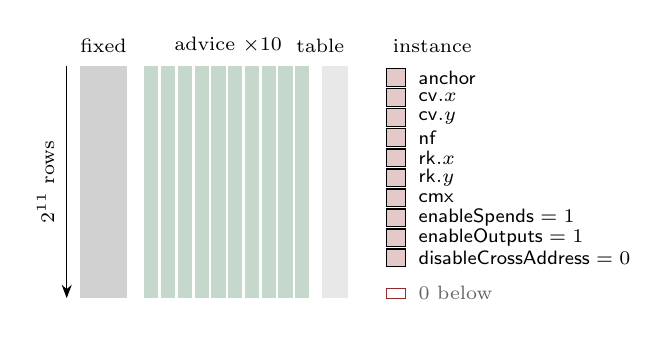
\begin{tikzpicture}[x=0.82cm,y=0.82cm,font=\scriptsize]
  \fill[arbdim!30] (0,0) rectangle ++(0.74,3.6);
  \node[anchor=south] at (0.37,3.65) {fixed};
  \foreach \i in {0,...,9}
    {\fill[arb!25] (1.0+\i*0.26,0) rectangle ++(0.22,3.6);}
  \node[anchor=south] at (2.3,3.65) {advice $\times 10$};
  \fill[arbdim!15] (3.75,0) rectangle ++(0.4,3.6);
  \node[anchor=south east] at (4.25,3.65) {table};
  \foreach \i in {0,...,9}
    {\draw[fill=arbred!25] (4.75,3.28-\i*0.31) rectangle ++(0.3,0.27);}
  \draw[arbred] (4.75,0) rectangle ++(0.3,0.15);
  \node[anchor=south west] at (4.7,3.65) {instance};
  \foreach \i/\l in {0/$\mathsf{anchor}$,1/$\cvsym.x$,2/$\cvsym.y$,
      3/$\nfsym$,4/$\rksym.x$,5/$\rksym.y$,6/$\cmx$,
      7/$\mathsf{enableSpends} = 1$,8/$\mathsf{enableOutputs} = 1$,
      9/$\mathsf{disableCrossAddress} = 0$}
    {\node[anchor=west] at (5.1,3.415-\i*0.31) {\l};}
  \node[anchor=west,text=arbdim] at (5.1,0.075) {$0$ below};
  \draw[-{Stealth}] (-0.2,3.6) -- (-0.2,0)
    node[midway,left=1pt,rotate=90,anchor=south] {$2^{11}$ rows};
\end{tikzpicture}}

\begin{board}{A zk-SNARK, precisely enough}{all four checks}
\Write
\begin{enumerate}
  \item Relation $R$: public statement $x$, private witness $w$.
  \item[] $\mathrm{Prove}(x, w) \to \pi, \qquad
    \mathrm{Verify}(x, \pi) \in \{0, 1\}$
  \item Knowledge sound: an extractor pulls a $w$ with $(x, w) \in R$
    out of any convincing prover.
  \item Zero knowledge: a simulator given only $x$ reproduces $\pi$.
  \item Schnorr $=$ proof of knowledge of $\log_G X$. SNARK $=$ the
    same, for any relation.
\end{enumerate}
\Say
\begin{itemize}
  \item In Bitcoin the validator holds everything it checks: the
    witness sits in the transaction. Here it holds only $x$ and a short
    $\pi$; the witness $w$ never leaves the prover.
  \item Plain soundness would allow ``a spendable note exists'' ---
    other people's notes exist. The extractor forces the prover to
    \emph{hold} a $w$.
  \item Here the relation is the ten clauses of the Action statement.
\end{itemize}
\end{board}

\begin{board}{Zero knowledge: what $\pi$ hides, and what it does not}
  {all four checks}
\Write
\begin{enumerate}
  \item Whatever a verifier learns from $\pi$, a simulator produces
    from $x$ alone.
  \item Published: $\nfsym$, $\rksym$, $\cvsym$, $\cmx$.
  \item Unlinkable because of: commitment hiding, the keyed nullifier
    PRF, key re-random\-isation --- not $\pi$.
  \item Zero knowledge: necessary, not sufficient. A perfect proof
    beside $\nfsym = \cmx$ hides nothing.
\end{enumerate}
\Say
\begin{itemize}
  \item The public inputs go on chain. That they cannot be linked back
    to the note and the key rests on Parts C and E, not on $\pi$.
  \item Bitcoin's witness is the secret's public shadow: a signature, a
    script preimage. Here the witness never leaves the prover; the
    shadow is the public-input tuple.
\end{itemize}
\end{board}

\begin{board}{Succinct, and non-interactive}{all four checks}
\Write
\begin{enumerate}
  \item Succinct: proof size logarithmic in the circuit ---
    commitments and openings, never the polynomials. One linear MSM,
    shared across a batch.
  \item[] $\text{challenge} := \mathrm{Hash}(\text{everything sent so
    far})$ \quad (Fiat--Shamir)
  \item Proof of knowledge $+$ Fiat--Shamir $=$ signature.
\end{enumerate}
\Say
\begin{itemize}
  \item Halo 2's verifier still pays one linear multi-scalar
    multiplication, shared across a batch: a SNARK in the proof-size
    sense.
  \item A commitment is an input of the hash, so it is fixed before the
    challenge that tests it exists. The proof becomes one static
    object; verification recomputes the hashes.
  \item A full node that has never met Alice verifies her Action long
    after it was made, from the proof string alone. Schnorr is
    Fiat--Shamir applied to the log relation.
\end{itemize}
\end{board}

\begin{board}{Arithmetisation: the claim becomes a table}
  {all four checks}
\begin{center}\small
\begin{tabular}{@{}c ccc ccccc c l@{}}
\toprule
& \multicolumn{3}{c}{advice} & \multicolumn{5}{c}{fixed} & instance & \\
\cmidrule(lr){2-4}\cmidrule(lr){5-9}\cmidrule(lr){10-10}
row & $a$ & $b$ & $c$ & $q_M$ & $q_L$ & $q_R$ & $q_O$ & $q_C$
  & $\mathrm{PI}$ & gate \\
\midrule
0 & 3 & 3 & 9 & 1 & 0 & 0 & $-1$ & 0 & 0 & $x \cdot x = x^2$ \\
1 & 9 & 3 & 27 & 1 & 0 & 0 & $-1$ & 0 & 0 & $x^2 \cdot x = x^3$ \\
2 & 27 & 3 & 30 & 0 & 1 & 1 & $-1$ & 0 & 0 & $x^3 + x = s$ \\
3 & 30 & 0 & 0 & 0 & 1 & 0 & 0 & 5 & $-35$ & $s + 5 = 35$ \\
\bottomrule
\end{tabular}
\end{center}
\Write
\begin{enumerate}
  \item Toy claim: ``I know $x$ with $x^3 + x + 5 = 35$'' over
    $\F_{97}$ ($x = 3$).
  \item[] $q_M\, a\, b + q_L\, a + q_R\, b + q_O\, c + q_C +
    \mathrm{PI} = 0$ \quad on every row
  \item Copy constraints: $a_0 = b_0 = b_1 = b_2$, $c_0 = a_1$,
    $c_1 = a_2$, $c_2 = a_3$.
  \item Range check $=$ lookup into a table, not algebra.
\end{enumerate}
\newpage
\Say
\begin{itemize}
  \item One operation per row, one gate equation evaluated on every
    row.
  \item Advice is the prover's secret trace. Fixed columns are the
    circuit: the selectors pick which operation a row performs. The
    instance column carries the public $35$.
  \item Copy constraints wire the rows: the $x$ in row 0 is the $x$ in
    rows 1 and 2; each row's output feeds the next.
  \item Bitcoin Script is executed by every validator; a circuit is
    never executed, only checked.
\end{itemize}
\Ask
Which column does the verifier never see?
\Answer
Advice: the prover's trace. Fixed columns are the circuit, known to
everyone; the instance column is the public $35$.
\end{board}

\begin{board}{Rows become polynomials}{all four checks}
\Write
\begin{enumerate}
  \item Roots of unity in $\F_{97}$: $\omega = 22$, $\omega^2 = 96 =
    -1$, $\omega^4 = 1$; row $i$ lives at $\omega^i \in H = \{1, 22,
    96, 75\}$.
  \item[] $a(1) = 3,\ a(22) = 9,\ a(96) = 27,\ a(75) = 30
    \ \Longrightarrow\ a(X) = 90 + 61X + 22X^2 + 24X^3$
  \item[] $G(X) := q_M a b + q_L a + q_R b + q_O c + q_C + \mathrm{PI},
    \qquad \deg G \le 9$
  \item[] every gate holds $\iff G(\omega^i) = 0$ for all $i$
    $\iff G$ vanishes on $H$
\end{enumerate}
\Say
\begin{itemize}
  \item The advice column $a$ becomes the unique polynomial of degree
    below $4$ through its four values: the column \emph{is} the
    polynomial, sampled at the rows. Likewise $b$, $c$ and the public
    columns.
  \item The value $G(\omega^i)$ is exactly row $i$'s gate equation.
  \item A Merkle root also folds many rows into one object, but it
    opens one leaf at a time; a polynomial can be probed anywhere.
\end{itemize}
\end{board}

\begin{board}{All rows at once: one identity, or none}{all four checks}
\Write
\begin{enumerate}
  \item[] $\wbGZH(X) := \prod_{h \in H}(X - h) = X^4 - 1$
  \item[] $G$ vanishes on $H \iff \wbGZH \mid G \iff G = t \cdot
    \wbGZH$
  \item Honest: $\deg G = 9$, $\deg t = 5$, remainder $0$.
  \item Cheat, $c_0 = 10$: row $0$ reads $3 \cdot 3 - 10 = -1 \neq 0$,
    so $\wbGZH \nmid G^{*}$.
  \item[] $D(X) := G^{*}(X) - t^{*}(X)\, \wbGZH(X) =
    24\,(1 + X + X^2 + X^3) \neq 0$
\end{enumerate}
\Say
\begin{itemize}
  \item Factor theorem, applied four times: $G$ vanishes on $H$ if and
    only if $\wbGZH$ divides $G$.
  \item A correct computation \emph{is} a polynomial identity; a wrong
    one cannot be. Copy constraints get the same treatment (a running
    product equal to $1$ when the wiring holds), and so do lookups.
  \item Bitcoin's validator checks each input's script on its own;
    here every row collapses into one identity that holds everywhere
    or fails almost everywhere.
\end{itemize}
\end{board}

\begin{board}{One random point: the protocol}{all four checks}
\Write
\begin{enumerate}
  \item Prover commits to $a, b, c$ and $t$; verifier knows $q_M,
    \dots, q_C$ and $\mathrm{PI}$.
  \item Transcript hash draws $z \in \F$ (Fiat--Shamir; BLAKE2b in the
    deployed transcript).
  \item Prover opens $a(z), b(z), c(z), t(z)$ with short proofs.
  \item Verifier forms $G(z)$, computes $\wbGZH(z) = z^4 - 1$, checks
  \item[] $G(z) \overset{?}{=} t(z)\, \wbGZH(z)$
  \item Honest, $z = 20$: $\wbGZH(20) = 46$, $t(20) = 67$, $G(20) = 75
    = 67 \cdot 46$. \checkmark
\end{enumerate}
\Say
\begin{itemize}
  \item Every honest prover passes at every $z$, because $G =
    t\,\wbGZH$ holds as polynomials.
  \item Bitcoin's validator re-executes the script; this one evaluates
    one equation at one point.
\end{itemize}
\end{board}

\begin{board}{One random point: why a lie is caught}{all four checks}
\Write
\begin{enumerate}
  \item Cheat: $D := G^{*} - t^{*} \wbGZH \neq 0$, frozen before $z$ is
    drawn.
  \item[] $\Pr_{z}[\text{cheat accepted}] = \Pr_z[D(z) = 0] \le
    \dfrac{\deg D}{|\F|}$ \quad (Schwartz--Zippel)
  \item Roots of $D = 24(1 + X + X^2 + X^3)$: $\{22, 75, 96\}$;
    $3/97$ for that $t^{*}$, $9/97$ for any admissible $t^{*}$.
  \item At $z = 20$: $G^{*}(20) = 20$ but $t^{*}(20)\,\wbGZH(20) =
    64$. Caught.
  \item Over $\Fpp$, $\deg D \approx 2^{14}$: about $2^{-240}$; the
    discrete-log layer gives about $126$ bits.
\end{enumerate}
\newpage
\Say
\begin{itemize}
  \item The commitments pin $G^{*}$ and $t^{*}$ before $z$ is drawn:
    $D$ is fixed, nonzero, with at most $\deg D$ roots.
  \item The $2^{-240}$ is one Schwartz--Zippel term, not the system's
    security level.
  \item A false statement disagrees with the truth almost everywhere;
    one probe lands where it disagrees.
\end{itemize}
\Ask
Why $3/97$ for this cheat but $9/97$ in general?
\Answer
This $D$ has exactly three roots, the rows where the tampered gate
still held; the general bound is $\deg D \le 9$.
\end{board}

\begin{board}{Committing to a polynomial: the problem}{all four checks}
\Write
\begin{enumerate}
  \item Needed: a short commitment $P$ to $f$, and a short proof that
    $f(x) = v$ at a drawn $x$ for the committed $f$.
  \item[] $P = \Comm(f; r) = \ip{\vec a}{\vec G} + [r]\,H \in \G$
  \item One Vesta point for $2^{11}$ coefficients. Binding under
    discrete log; hiding by $[r]H$; no secret behind $\vec G$.
  \item Merkle: one entry in $\log_2 d$ hashes. IPA: a combination of
    all entries in $2\log_2 d$ points.
\end{enumerate}
\Say
\begin{itemize}
  \item The random-point argument assumed the polynomials were pinned
    before $z$ was drawn.
  \item Pedersen, vectorised: commit to the coefficient vector with
    generators $\vec G$ and $H$ hashed into existence.
\end{itemize}
\end{board}

\begin{board}{Committing to a polynomial: the opening claim}
  {all four checks}
\Write
\begin{enumerate}
  \item[] $f(x) = \ip{\vec a}{\vec b(x)}, \qquad \vec b(x) := (1, x,
    x^2, \dots, x^{d-1})$
  \item[] $P + [v]\,U = \ip{\vec a}{\vec G} + [r]\,H +
    [\ip{\vec a}{\vec b}]\,U$
  \item Sending $\vec a$: $d$ elements. Inner-product argument:
    $2\log_2 d$ points, $22$ for $d = 2^{11}$.
\end{enumerate}
\Say
\begin{itemize}
  \item Evaluation is an inner product. With a second hashed generator
    $U$, the opening claim becomes one group equation.
  \item The inner-product argument is the Bulletproofs family known
    from range proofs.
  \item A Merkle proof names one leaf; an IPA opening is one number
    computed from every coefficient, at a point chosen after they were
    fixed.
\end{itemize}
\Ask
How many points does the opening cost for $d = 2^{11}$?
\Answer
$2 \log_2 d = 22$.
\end{board}

\begin{board}{The inner-product argument: one fold}{all four checks}
\Write
\begin{enumerate}
  \item Split: $\vec a = (\wbGlo{\vec a}, \wbGhi{\vec a})$, likewise
    $\vec G$ and $\vec b$.
  \item[] $L := \ip{\wbGlo{\vec a}}{\wbGhi{\vec G}} + [\ell]\,H
      + [\ip{\wbGlo{\vec a}}{\wbGhi{\vec b}}]\,U$
  \item[] $R := \ip{\wbGhi{\vec a}}{\wbGlo{\vec G}} + [r_R]\,H
      + [\ip{\wbGhi{\vec a}}{\wbGlo{\vec b}}]\,U$
  \item Challenge $u$; fold:
  \item[] $\vec a' := u\,\wbGlo{\vec a} + u^{-1}\wbGhi{\vec a}, \quad
    \vec G' := u^{-1}\wbGlo{\vec G} + u\,\wbGhi{\vec G}, \quad
    \vec b' := u^{-1}\wbGlo{\vec b} + u\,\wbGhi{\vec b}$
  \item[] $\ip{\vec a'}{\vec G'} = \ip{\vec a}{\vec G} +
    u^2 \ip{\wbGlo{\vec a}}{\wbGhi{\vec G}} +
    u^{-2} \ip{\wbGhi{\vec a}}{\wbGlo{\vec G}}$
  \item[] $P + [v]\,U + [u^2]\,L + [u^{-2}]\,R
    = \ip{\vec a'}{\vec G'} + [r + u^2 \ell + u^{-2} r_R]\,H
    + [\ip{\vec a'}{\vec b'}]\,U$
\end{enumerate}
\Say
\begin{itemize}
  \item Both parties fold in step: the prover folds $\vec a$ with
    weights $(u, u^{-1})$, the verifier folds $\vec G$ and $\vec b$
    with the inverse weights, by public arithmetic, never seeing
    $\vec a$.
  \item The old claim plus $[u^2]L + [u^{-2}]R$ is the same claim at
    half the length.
  \item This is the textbook (Bulletproofs) form; a Bulletproofs range
    proof folds its vectors by exactly this move.
\end{itemize}
\end{board}

\begin{board}{The inner-product argument: the recursion}
  {all four checks}
\Write
\begin{enumerate}
  \item After $k = \log_2 d$ rounds every vector has length $1$.
  \item Proof: $2k$ points $(L_j, R_j)$, final scalar $a$, blinder
    $r^{*} = r + \sum_j (u_j^2 \ell_j + u_j^{-2} r_j)$.
  \item[] $P + [v]\,U + \sum_{j=1}^{k}\bigl([u_j^2]\,L_j +
    [u_j^{-2}]\,R_j\bigr) \overset{?}{=} [a]\,G^{(0)} + [r^{*}]\,H +
    [a \cdot b^{(0)}]\,U$
  \item[] $b^{(0)} = \prod_{\ell}(u_\ell^{-1} + u_\ell\,
    x^{2^{\ell-1}})$ \quad $O(\log d)$ field operations
  \item[] $G^{(0)} = \ip{\vec s}{\vec G}$ \quad an MSM of length $d$
\end{enumerate}
\Say
\begin{itemize}
  \item The verifier accumulates the cross terms into the commitment
    and checks one group equation.
  \item The point $G^{(0)}$ is the one linear step; the node shares it
    across a batch. Recursion would defer it into an accumulator,
    which is not deployed.
  \item Binding: two openings of one commitment would exhibit a
    non-trivial discrete-log relation among $\vec G, H$ on Vesta.
\end{itemize}
\end{board}

\begin{board}{What the fold hides, and the deployed normalisation}
  {all four checks}
\Write
\begin{enumerate}
  \item Folding alone is not zero knowledge: the final $a$ is a
    challenge-dependent linear form in the coefficients.
  \item Deployed: mask $f$ by a random polynomial vanishing at the
    opening point, commit as $S$, draw two more challenges, then fold.
  \item Deployed weights: $(1, u_j^{-1})$ on coefficients, $(1, u_j)$
    on $\vec b$ and $\vec G$; accumulate $[u_j^{-1}]\,L_j + [u_j]\,R_j$.
  \item Same $2k$ points, plus $S$ and two final scalars.
\end{enumerate}
\Say
\begin{itemize}
  \item Blinding $P$ and the round points hides those points, not $a$.
  \item The two conventions are related by per-round rescaling; the
    previous board's form is the textbook one.
  \item A Bitcoin signature exposes its public key by design; here
    even the last scalar of an opening must be masked.
\end{itemize}
\end{board}

\begin{board}{The fold by hand: two rounds}{all four checks}
\Write
\begin{enumerate}
  \item Toy: $p(X) = 5 + X + X^3$ opened at $x = 3$, so $v = 35$.
    Group: $\mathbb{Z}_{97}$ written additively, $[k]G = kG \bmod 97$.
  \item[] $\vec a = (5, 1, 0, 1), \quad \vec b = (1, 3, 9, 27), \quad
    \vec G = (2, 3, 5, 7)$
  \item[] $H = 11, \quad U = 13, \quad r = 17, \qquad
    P = \ip{\vec a}{\vec G} + [r]H = 13$
\end{enumerate}
\smallskip
{\centering\small
\begin{tabular}{@{}l ccc ccc c@{}}
\toprule
round & $L_j$ & $R_j$ & $u_j$ & $\vec a'$ & $\vec b'$ & $\vec G'$
  & fold check \\
\midrule
$j = 2$ ($\ell_2, r_2 = 19, 23$) & $13$ & $4$ & $3$ & $(15, 68)$
  & $(92, 82)$ & $(48, 22)$ & $25 = 25$ \\
$j = 1$ ($\ell_1, r_1 = 29, 31$) & $52$ & $58$ & $5$ & $(11)$ & $(21)$
  & $(42)$ & $12 = 12$ \\
\bottomrule
\end{tabular}\par}
\smallskip
\begin{enumerate}[resume]
  \item Fold check per row: $\ip{\vec a'}{\vec G'} + [r^{*}]H +
    [\ip{\vec a'}{\vec b'}]U = P + [v]U + [u^2]L + [u^{-2}]R$.
\end{enumerate}
\Say
\begin{itemize}
  \item The stand-in group $\mathbb{Z}_{97}$ has no discrete-log
    hardness; the numbers show only the fold's algebra. Each row's
    check is the one-fold identity, instantiated.
\end{itemize}
\end{board}

\begin{board}{The fold by hand: the final check}{all four checks}
\Write
\begin{enumerate}
  \item Prover sends $a = 11$ and $r^{*} = 30$.
  \item[] $\vec s = (u_1^{-1}u_2^{-1},\ u_1 u_2^{-1},\ u_1^{-1}u_2,\
    u_1 u_2) = (13, 34, 20, 15), \qquad G^{(0)} = \ip{\vec s}{\vec G}
    = 42$
  \item[] $b^{(0)} = g(x; u_1, u_2) = (u_1^{-1} + u_1 x)(u_2^{-1} + u_2
    x^2) = 21$
  \item[] $P + [v]U + [u_1^2]L_1 + [u_1^{-2}]R_1 + [u_2^2]L_2 +
    [u_2^{-2}]R_2 = 12$
  \item[] $[a]\,G^{(0)} + [r^{*}]\,H + [a \cdot b^{(0)}]\,U = 12$
\end{enumerate}
\Say
\begin{itemize}
  \item The verifier works from the challenges alone: $\vec s$,
    $G^{(0)}$ and $b^{(0)}$ need nothing from the prover.
  \item Both sides come to $12$: accepted. Four coefficients were never
    sent; four points and two scalars were.
  \item On Vesta the same equations are hiding and binding, and
    $G^{(0)}$ is a length-$2^{11}$ multi-scalar multiplication.
\end{itemize}
\end{board}

\begin{board}{Fields and curves in the deployed circuit}
  {all four checks}
\Write
\begin{enumerate}
  \item Native field: $\Fpp$, the \emph{base} field of Pallas.
  \item Native points: $\cmsym$, $\rksym$, $\cvsym$, $\aksym$, $\pkd$
    --- coordinates in $\Fpp$, group law by native arithmetic.
  \item Column polynomials committed on Vesta, whose \emph{scalar}
    field is exactly $\Fpp$.
\end{enumerate}
\Say
\begin{itemize}
  \item The group law is native arithmetic, not emulated; the
    committed coefficients are the circuit's own field elements.
  \item Bitcoin's secp256k1 is one curve doing one job: its validator
    verifies signatures, never circuits.
\end{itemize}
\end{board}

\begin{board}{The Pasta cycle, once}{all four checks}
\Write
\begin{enumerate}
  \item Pallas over $\Fpp$ has order $p_{\Vesta}$; Vesta over $\Fpv$
    has order $p_{\Pallas}$.
  \item Vesta-committed proof: Vesta points, coordinates in $\Fpv$
    $\to$ verified natively by a circuit over $\Fpv$, committed on
    Pallas.
  \item Its proof: Pallas points, coordinates in $\Fpp$ $\to$ verified
    natively by a circuit over $\Fpp$, committed on Vesta.
  \item Not deployed: the node verifies each bundle's proof directly
    and batches the deferred MSMs.
\end{enumerate}
\Say
\begin{itemize}
  \item Each curve's scalar field is the other's base field: that is
    the whole definition of the cycle.
  \item Proofs alternate between the two curves, each verifier a
    circuit, so one proof can attest to the previous one.
  \item Bitcoin needs no such pair; a signature is verified by
    arithmetic, not by another proof.
\end{itemize}
\end{board}

\begin{board}{Why not Bitcoin's curve: two-adicity}{all four checks}
\begin{center}\small
\begin{tabular}{@{}lccc@{}}
\toprule
field & bits & two-adicity of $p - 1$ & largest domain \\
\midrule
$\Fpp$ (Pallas base) & $255$ & $32$ & $2^{32}$ \\
$\Fpv$ (Vesta base) & $255$ & $32$ & $2^{32}$ \\
secp256k1 base field & $256$ & $1$ & $2$ \\
secp256k1 scalar field & $256$ & $6$ & $64$ \\
\bottomrule
\end{tabular}
\end{center}
\Write
\begin{enumerate}
  \item Interpolating over $n = 2^{11}$ rows needs a primitive
    $2^{11}$-th root of unity: $2^{11} \mid p - 1$.
  \item Quotient FFTs run on $8n = 2^{14}$ points at the deployed gate
    degree.
  \item Two-adicity: the largest $k$ with $2^k \mid p - 1$.
  \item Bitcoin's prime $p = 2^{256} - 2^{32} - 977$: $p - 1$ is twice
    an odd number, a domain of two points.
\end{enumerate}
\newpage
\Say
\begin{itemize}
  \item The Pasta primes were designed for this: two-adicity exactly
    $32$ in both, so domains of every size up to $2^{32}$.
  \item The secp256k1 curve buys its implementation speed from
    $a = 0$; its prime was not chosen for evaluation domains.
\end{itemize}
\Ask
Could secp256k1's base field host even the four-row toy?
\Answer
No: two-adicity $1$, largest domain two points.
\end{board}

\begin{board}{Trust: what a ceremony is, and why there is none}
  {conserved}
\Write
\begin{enumerate}
  \item[] $pp = \bigl([\tau^0]G, [\tau^1]G, \dots, [\tau^d]G,
    \dots\bigr), \qquad \tau \text{ destroyed}$
  \item Whoever keeps $\tau$ forges: for any $C$, $z$, $y$,
  \item[] $\pi := [(\tau - z)^{-1}]\,(C - [y]G)$ \quad passes, no
    polynomial behind it --- the toxic waste.
  \item Groth16: secrets per circuit. MPC: safe if \emph{one}
    participant destroyed their share. The Sapling pool still rests on
    that.
  \item Bound (ZIP-209): each pool's chain value balance is public and
    may not go negative $\Rightarrow$ counterfeit capped at the pool's
    exit.
  \item Orchard, Ironwood: IPA generators hashed from a public domain
    tag; nothing to leak, nothing to destroy.
\end{enumerate}
\Say
\begin{itemize}
  \item A forged Sapling proof creates value only inside the Sapling
    pool and can withdraw at most what that pool publicly holds ---
    the turnstile, Part H.
  \item Bitcoin never had a setup; Sapling has one; Orchard returns to
    none.
\end{itemize}
\end{board}

\begin{board}{Three generations}{all four checks}
\begin{center}\small
\begin{tabular}{@{}llll@{}}
\toprule
& Sprout & Sapling & Orchard, Ironwood \\
\midrule
SNARK & BCTV14 (original) & Groth16 & Halo 2 \\
curve & BN254 & BLS12-381, Jubjub in-circuit & Pallas, Vesta \\
setup & six-party MPC & large MPC & none \\
hash in circuit & SHA-256 & Pedersen & Sinsemilla \\
proof & 296 B & 192 B & $2720 + 2272a$ B \\
verification & constant & three pairings & $O(\log n)$ + shared MSM \\
\bottomrule
\end{tabular}
\end{center}
\Write
\begin{enumerate}
  \item Sprout: BCTV14 soundness flaw found after deployment; re-proved
    with Groth16, deprecated.
  \item Sapling: Groth16 over BLS12-381, Jubjub inside the circuit.
  \item Orchard: proof grows because transparency costs $2\log_2 n$
    points.
\end{enumerate}
\newpage
\Say
\begin{itemize}
  \item Sapling: a far faster prover, a per-circuit ceremony, no curve
    cycle.
  \item Bitcoin changed its signature scheme once, by opt-in; Zcash has
    carried shielded payments through three proof systems, each with
    its own pool --- the third with two, Orchard and Ironwood, on one
    circuit.
\end{itemize}
\end{board}

\begin{board}{The Orchard circuit by the numbers}{all four checks}
\begin{center}\small
\begin{tabular}{@{}ll@{}}
\toprule
rows & $2^{11} = 2048$; one fixed circuit, every Action an
  instance \\
columns & ten advice, fixed columns, a Sinsemilla lookup table \\
proof per bundle & $2720 + 2272\,a$ B: $4992$ for one Action, $7264$
  for Alice's two \\
of which IPA & $22$ pair points and one blinding commitment, $32$ B
  each \\
proving & a few seconds on commodity hardware \\
verifying & $O(\log n)$ per proof, plus one MSM shared across a batch \\
\bottomrule
\end{tabular}
\end{center}
\newpage
\Write
\begin{enumerate}
  \item One aggregate proof per bundle: per-Action term $=$ that
    Action's column commitments and evaluations; constant term $=$ the
    shared quotient, multipoint and IPA data.
  \item Spend-auth signature: $64$ B. One-Action proof: $78$
    signatures' worth.
\end{enumerate}
\Say
\begin{itemize}
  \item Bitcoin's witness cost is per input and grows with the script
    it satisfies; here it is per bundle, logarithmic in the circuit,
    and independent of the anonymity set.
\end{itemize}
\end{board}

\begin{board}{Five gadget families, three circuit versions}
  {all four checks}
\Write
\begin{enumerate}
  \item ECC: $\rksym = \aksym + [\alpha]\,G^{\mathsf{SpendAuth}}$ (A6),
    $\pkd = [\ivk]\,\gd$ (A7), $\cvsym$ (A4), the nullifier's point
    (A5).
  \item Sinsemilla: generator table as a lookup; per $10$-bit chunk one
    lookup and two incomplete additions; $\NoteCommit$ (A1, A2),
    $\CommitIvk$ (A7).
  \item Merkle path: $32$ layer-tagged hashes, a conditional swap per
    layer by one bit of the position, root $=$ anchor gated by
    $v_{\mathrm{old}}$ (A3).
  \item Poseidon: the nullifier PRF; only non-linearity $x \mapsto x^5$
    (A5).
  \item Decomposition: $v \in [0, 2^{64})$ and the sign bit (A4);
    canonicity of witnessed encodings.
  \item Three versions: original, a correction, the Ironwood circuit
    with the cross-address input. Verifying key selected by branch.
\end{enumerate}
\newpage
\Say
\begin{itemize}
  \item Canonicity of witnessed encodings is distinct from the node's
    parsing of public encodings, Part E.
  \item Consensus selects the verifying key by branch, so every Action
    in either pool now verifies against the Ironwood key.
  \item Bitcoin's validator runs whatever script an output declares;
    this one runs a verifier keyed to one fixed circuit.
\end{itemize}
\end{board}

\begin{board}{Alice's Action as an instance}{all four checks}
\begin{center}
\resizebox{!}{0.6\textheight}{\wbGInstanceFig}
\end{center}
\newpage
\Write
\begin{enumerate}
  \item Instance (Action 1: $2$ ZEC $\to$ Bob $1.5$): eight public
    inputs, ten field elements; points by coordinates; flags as the
    Ironwood component sets them.
  \item Advice: both notes; $32$ siblings and the position; $\aksym$,
    $\nksym$, $\rivk$, $\ivk$; $\alpha$; $\rcv$;\\
    $(\mathrm{magnitude}, \mathrm{sign}) = (50\,000\,000, +1)$.
  \item Copy constraints tie each instance cell to the advice cell
    holding the same value.
\end{enumerate}
\Say
\begin{itemize}
  \item The verifier computes the instance commitment itself, so a
    proof for other values fails the opening.
  \item Bitcoin's witness --- scriptSig or witness field --- is in the
    clear; here the witness fills advice cells nobody reads.
\end{itemize}
\Ask
Checkpoint: what could a holder of the Sapling ceremony's toxic waste
do, what stops the analogue in Orchard, and what bounds the damage?
\Answer
\begin{itemize}
  \item Forge accepting Sapling proofs of false statements: counterfeit
    inside the Sapling pool, invisible to every verifier. Not decrypt
    notes --- soundness and zero knowledge are separate guarantees.
  \item In Orchard there is no trapdoor to hold: the generators are
    hashed, and binding reduces to discrete log.
  \item Under ZIP-209 each pool's chain value balance is public, and a
    block that would drive it negative is invalid --- counterfeit is
    capped at the pool's exit.
\end{itemize}
\end{board}

%% ---- 08-delivery.tex
%% Part F --- Delivery and light clients (screen version)
%% Derived from wb/08-delivery.tex; numbers unchanged.

\newcommand{\wbFenc}{\ensuremath{C_{\mathrm{enc}}}}
\newcommand{\wbFout}{\ensuremath{C_{\mathrm{out}}}}
\newcommand{\wbFnp}{\ensuremath{\mathsf{np}}}
\newcommand{\wbFrseed}{\ensuremath{\mathsf{rseed}}}
\newcommand{\wbFock}{\ensuremath{\mathsf{ock}}}
\newcommand{\wbFpre}{\ensuremath{\mathsf{pre}_{\rcm}}}
\newcommand{\wbFivkint}{\ensuremath{\ivk^{\mathsf{int}}}}
\newcommand{\wbFkenc}{\ensuremath{K_{\mathrm{enc}}}}

\section{Part F --- Delivery and light clients}

\begin{board}{The note plaintext: what travels to Bob}{exists}
\Write
\begin{enumerate}
  \item $\wbFnp := (\mathtt{0x03},\ d,\ v,\ \wbFrseed,\ \mathsf{memo})$
  \item $1 + 11 + 8 + 32 + 512 = 564$ bytes
  \item $\wbFrseed \to \esk$ \quad
    ($\mathsf{PRFexpand}_{\wbFrseed}(\mathtt{0x04} \,\|\, \rho)$)
  \item $\wbFrseed \to \psi$ \quad
    ($\mathsf{PRFexpand}_{\wbFrseed}(\mathtt{0x09} \,\|\, \rho)$)
  \item $\wbFrseed \to \rcm$ \quad (next board)
  \item $\rho := \nfsym_{\mathrm{old}}$
\end{enumerate}
\Say
\begin{itemize}
  \item The chain stores only \cmx; Alice delivers the note plaintext to
    Bob herself.
  \item Lead byte $\mathtt{0x03}$ is the Ironwood note, the only value
    the Ironwood pool admits.
  \item The 32-byte seed is the note's whole randomness; $\rho :=
    \nfsym_{\mathrm{old}}$ binds it to its Action. The memo never
    appears in the clear.
  \item Bitcoin: amount and script are public, and so is an OP\_RETURN
    note.
\end{itemize}
\end{board}

\begin{board}{The Ironwood trapdoor: one hash over every note field}{exists}
\Write
\begin{enumerate}
  \item Ironwood pool ($\mathtt{0x03}$):
    $\rcm := \mathrm{ToScalar}\bigl(\mathsf{PRFexpand}_{\wbFrseed}(
      \wbFpre)\bigr)$
  \item $\wbFpre := \mathtt{0x0B} \,\|\, \gd^\star \,\|\, \pkd^\star
    \,\|\, \mathrm{LE}_{64}(v) \,\|\, \mathrm{LE}_{256}(\rho) \,\|\,
    \mathrm{LE}_{256}(\psi)$
  \item $1 + 32 + 32 + 8 + 32 + 32 = 137$ bytes
  \item Orchard pool ($\mathtt{0x02}$):
    $\rcm := \mathrm{ToScalar}\bigl(\mathsf{PRFexpand}_{\wbFrseed}(
      \mathtt{0x05} \,\|\, \mathrm{LE}_{256}(\rho))\bigr)$
  \item $1 + 32 = 33$ bytes
\end{enumerate}
\Say
\begin{itemize}
  \item The one note-level difference between the pools is how \rcm{}
    leaves the seed; \esk{} and $\psi$ are byte-identical, and the lead
    byte says which derivation applies.
  \item Every note field enters the Ironwood preimage, so \rcm{} is
    derived last, after $\psi$.
  \item The commitment is unchanged: same \NoteCommit, same tree
    construction, each pool its own instance (ZIP-229).
  \item Bitcoin: an output has no trapdoor; there is nothing hidden to
    bind.
\end{itemize}
\end{board}

\begin{board}{Why the detour through BLAKE2b: post-quantum binding}{exists}
\Write
\begin{enumerate}
  \item Sinsemilla binding $=$ discrete log $\to$ falls to a quantum
    computer
  \item $\mathsf{PRFexpand}$ as a random oracle; every field enters
    $\wbFpre$
  \item derivation $+$ \NoteCommit{} $=$ post-quantum binding
  \item \emph{provided a verifier checks the derivation} --- no deployed
    clause does
  \item Ironwood note: recoverable; Orchard-/Sapling-pool note: not
\end{enumerate}
\Say
\begin{itemize}
  \item Sinsemilla collision resistance binds \NoteCommit; a large
    quantum computer breaks it (Part I), and then \NoteCommit{} alone
    binds nothing.
  \item Any change to a committed note re-randomises \rcm; two honest
    note--trapdoor pairs on one commitment is an oracle collision, with
    no group structure for Shor.
  \item The claim is conditional on a future verifier check of the
    derivation. This is what makes an Ironwood note recoverable (Parts
    H and I).
  \item Bitcoin: nothing in an output is hidden, so nothing must stay
    bound after a break.
\end{itemize}
\end{board}

\begin{board}{Sealing the note: one-shot Diffie--Hellman, then an AEAD}{exists}
\Write
\begin{enumerate}
  \item Bob's address $(d, \pkd)$, \quad $\gd = \GroupHash(d)$, \quad
    $\pkd = [\ivk]\,\gd$
  \item $\epk := [\esk]\,\gd$
  \item $\mathsf{s} := [\esk]\,\pkd$
  \item $\wbFkenc := \mathsf{KDF}(\mathsf{s},\ \epk)$
  \item $\wbFenc := \mathsf{Enc}_{\wbFkenc}(\wbFnp)$ \quad
    $564 + 16\text{-byte tag} = 580$ bytes
  \item $[\ivk]\,\epk = [\ivk][\esk]\,\gd = [\esk]\,\pkd = \mathsf{s}$
\end{enumerate}
\Say
\begin{itemize}
  \item KDF: BLAKE2b-256 over the encodings of $\mathsf{s}$ and \epk.
    AEAD: ChaCha20-Poly1305, fixed all-zero nonce, empty associated
    data --- a fresh key for every note.
  \item Bob (with \ivk) and Alice (with \esk) both reach $\mathsf{s}$;
    either recovers \wbFkenc{} from the published $(\epk, \wbFenc)$.
  \item Bitcoin: BIP-352 runs the same ECDH (input keys as \esk, no
    \epk) to derive an output key shown in the clear; here the shared
    secret encrypts the note, memo included.
\end{itemize}
\end{board}

\begin{board}{The second ciphertext: the sender's own copy}{exists}
\Write
\begin{enumerate}
  \item $\wbFock := \mathrm{BLAKE2b\text{-}256}\bigl(\ovk \,\|\, \cvsym
    \,\|\, \cmx \,\|\, \epk\bigr)$
  \item $\wbFout := \mathsf{Enc}_{\wbFock}(\pkd,\ \esk)$ \quad
    $64 + 16 = 80$ bytes
  \item \ovk{} holder: $\mathsf{s} = [\esk]\,\pkd$ $\to$ reads the note
    as Bob does
  \item $\ovk = \bot$ $\to$ random bytes under a random key
  \item Action publishes $(\epk, \wbFenc, \wbFout)$ beside
    $\cvsym, \nfsym, \rksym, \cmx$
\end{enumerate}
\Say
\begin{itemize}
  \item Eighty bytes buy a sent history: from $(\pkd, \esk)$ the holder
    of \ovk{} re-derives $\mathsf{s}$ and reads the note as Bob does.
  \item Binding \cvsym, \cmx, \epk{} into \wbFock{} ties \wbFout{} to
    its own Action; with $\ovk = \bot$ no outgoing key ever opens it.
  \item The node never opens any of the three; no clause of the Action
    statement mentions them.
  \item Bitcoin: the chain is the sender's copy; here a sent history
    needs a kept key.
\end{itemize}
\end{board}

\begin{board}{Finding your money: detection is successful decryption}{exists}
\Write
\begin{enumerate}
  \item for \emph{every} Orchard-protocol output:
  \item $\mathsf{s} := [\ivk]\,\epk$, \quad
    $\wbFkenc := \mathsf{KDF}(\mathsf{s},\ \epk)$, \quad
    $\wbFnp := \mathsf{Dec}_{\wbFkenc}(\wbFenc)$
  \item tag rejects a wrong key $\to$ an open is a \emph{candidate}
  \item check 1: \esk{} from \wbFrseed, \quad $[\esk]\,\gd = \epk$
  \item check 2: note from $(d, v, \wbFrseed)$ and
    $\rho := \nfsym_{\mathrm{old}}$, \quad
    $\Extract(\NoteCommit_{\rcm}(\ldots)) = \cmx$
  \item cost: one key agreement per output per \ivk{} $+$ every
    output's bandwidth
\end{enumerate}
\Say
\begin{itemize}
  \item Nothing on chain names a recipient, so there is nothing to ask
    for: Bob's wallet trial-decrypts every Orchard-protocol output with
    \ivk.
  \item An open is a candidate, not yet a note; the two re-derivations
    close the obvious forgeries.
  \item The cost is a count, not a clock. One \ivk{} scans both pools.
  \item Bitcoin: a lookup over public scripts; here, a decryption
    attempt on every output.
\end{itemize}
\end{board}

\begin{board}{Compact blocks (ZIP-307): what a light client downloads}{exists,
  not twice}
\begin{center}
\resizebox{0.85\textwidth}{!}{%
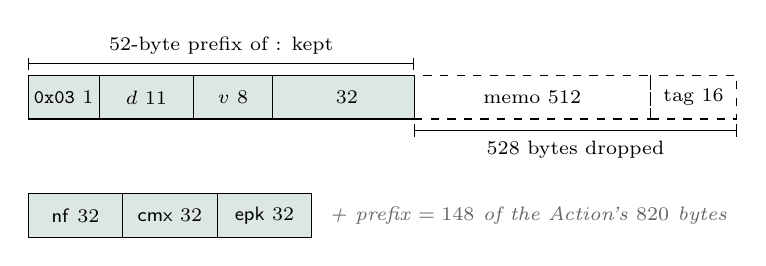
\begin{tikzpicture}[every node/.style={font=\scriptsize},
  b/.style={draw,minimum height=5.5mm,inner sep=2pt,outer sep=0pt,
    anchor=west}]
\node[b,fill=arb!15,minimum width=9mm] (l) at (0,0) {$\mathtt{0x03}$ 1};
\node[b,fill=arb!15,minimum width=12mm] (d) at (l.east) {$d$ 11};
\node[b,fill=arb!15,minimum width=10mm] (v) at (d.east) {$v$ 8};
\node[b,fill=arb!15,minimum width=18mm] (r) at (v.east) {\wbFrseed{} 32};
\node[b,dashed,minimum width=30mm] (m) at (r.east) {memo 512};
\node[b,dashed,minimum width=11mm] (t) at (m.east) {tag 16};
\draw[|-|] ([yshift=1.5mm]l.north west) -- ([yshift=1.5mm]r.north east)
  node[midway,above] {$52$-byte prefix of \wbFenc: kept};
\draw[|-|] ([yshift=-1.5mm]m.south west) -- ([yshift=-1.5mm]t.south east)
  node[midway,below] {$528$ bytes dropped};
\node[b,fill=arb!15,minimum width=12mm] (nf) at (0,-1.5) {\nfsym{} 32};
\node[b,fill=arb!15,minimum width=12mm] (cm) at (nf.east) {\cmx{} 32};
\node[b,fill=arb!15,minimum width=12mm] (ep) at (cm.east) {\epk{} 32};
\node[anchor=west,font=\scriptsize\itshape,text=arbdim] at (ep.east)
  {\ + prefix $= 148$ of the Action's $820$ bytes};
\end{tikzpicture}}
\end{center}
\Write
\begin{enumerate}
  \item compact Action $= \nfsym \,\|\, \cmx \,\|\, \epk \,\|\,
    \wbFenc[0..52)$
  \item $3 \cdot 32 + 52 = 148$ of $820$ bytes
  \item dropped: memo, tag, \wbFout, \cvsym, \rksym, anchor, proof,
    signatures
  \item per block, per pool: end-of-block tree size
\end{enumerate}
\Say
\begin{itemize}
  \item A compact block keeps only what three tasks need: detect a
    payment, detect a spend of one's own notes, update witnesses.
  \item Bitcoin: an SPV client downloads headers and asks for what
    matches; this client downloads every compact block in range and
    asks for no particular output.
\end{itemize}
\end{board}

\begin{board}{Accepting a note without its tag}{exists}
\Write
\begin{enumerate}
  \item $\wbFnp := \mathsf{ciphertext}[0..52) \;\oplus\;
    \mathsf{ChaCha20}_{\wbFkenc}(\mathrm{nonce} = 0)[64..116)$
  \item bare keystream, past block $0$ (the tag key's block)
  \item accept iff: 1. the 52 bytes parse as a compact note plaintext;
    2. recomputed commitment $=$ served \cmx; 3. \esk{} from \wbFrseed{}
    reproduces \epk
  \item commitment binding stands in for the tag
\end{enumerate}
\Say
\begin{itemize}
  \item Truncation at 52 bytes discards the Poly1305 tag, so the wallet
    applies the bare keystream past block $0$, which the full AEAD
    reserves for the tag key.
  \item Bob holds neither \cvsym{} nor the binding signature; under
    commitment binding, no sender can make him accept a note the chain
    did not commit to.
  \item Bitcoin: BIP-37 hands each peer a Bloom filter of the wallet's
    scripts; BIP-157 matches a per-block filter locally, then fetches
    the matching blocks. Here the ``filter'' is \ivk, applied to every
    block, and no match is ever requested.
\end{itemize}
\end{board}

\begin{board}{Leaks, in both directions}{none --- privacy of the scan}
\Write
\begin{enumerate}
  \item scan stage: \textbf{less} --- every compact block in range
    fetched; server sees range bounds $+$ timing, never a per-block
    match
  \item after detection: \textbf{more} --- full-transaction fetch names
    an exact txid (BIP-157: a whole block)
  \item ZIP-307 on that fetch: decoys (SHOULD); every transaction of
    any block touched (SHOULD); tell the user (MUST)
  \item deployed libraries: no decoy policy
\end{enumerate}
\Say
\begin{itemize}
  \item A BIP-157 client reveals each block it fetches after a filter
    hit; here the server never sees a per-block match.
  \item The memo and \wbFout{} live in the full transaction, which
    compact blocks omit.
  \item Structural: asking for ranges reveals where the client stopped;
    fetching what it detected reveals what it detected.
\end{itemize}
\end{board}

\begin{board}{Placing the note: a position from public data}{exists,
  not twice}
\Write
\begin{enumerate}
  \item $\mathrm{pos}(\text{output } i \text{ of } tx) =
    \text{start-of-block size} + \mathrm{offset}(tx) + i$
  \item start size $=$ stated end-of-block size $-$ the block's own
    outputs
  \item $\mathrm{offset}(tx) =$ outputs of the block's earlier
    transactions
  \item append \emph{every} \cmx; mark own
  \item spend: every compact \nfsym{} vs own unspent nullifiers, locally
\end{enumerate}
\Say
\begin{itemize}
  \item Trial decryption tells Bob that an output is his; the tree needs
    to know where. The position is arithmetic on public data, never a
    replay.
  \item The stated size is load-bearing: a note without a position has
    no witness.
  \item Bitcoin: an SPV client's branch arrives because its filter
    (BIP-37), its block fetch (BIP-157), or --- on Electrum --- the
    txid itself named its interest. Bob names nothing.
\end{itemize}
\end{board}

\begin{board}{Shards and the cap: a witness without the whole tree}{exists}
\begin{center}
\resizebox{0.8\textwidth}{!}{%
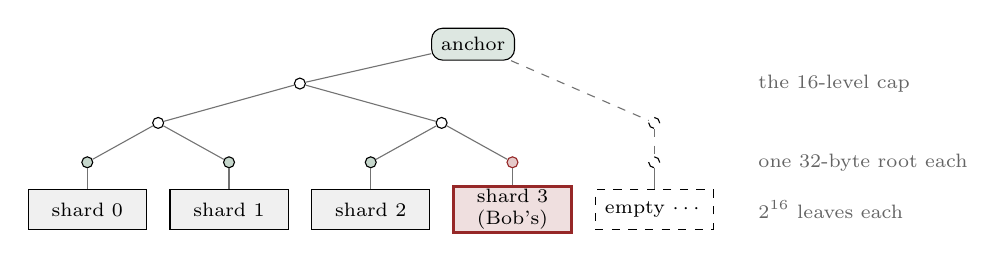
\begin{tikzpicture}[x=1mm,y=1mm,every node/.style={font=\scriptsize},
  sh/.style={draw,minimum width=15mm,minimum height=5mm,inner sep=1pt,
    align=center},
  rt/.style={draw,circle,inner sep=1.4pt},
  ed/.style={black!55}]
\node[sh,fill=black!6] (s0) at (0,0) {shard $0$};
\node[sh,fill=black!6] (s1) at (18,0) {shard $1$};
\node[sh,fill=black!6] (s2) at (36,0) {shard $2$};
\node[sh,fill=arbred!15,draw=arbred,very thick] (s3) at (54,0)
  {shard $3$\\ (Bob's)};
\node[sh,dashed] (s4) at (72,0) {empty $\cdots$};
\node[rt,fill=arb!25] (r0) at (0,6) {};
\node[rt,fill=arb!25] (r1) at (18,6) {};
\node[rt,fill=arb!25] (r2) at (36,6) {};
\node[rt,fill=arbred!25,draw=arbred] (r3) at (54,6) {};
\node[rt,dashed] (r4) at (72,6) {};
\node[rt] (a) at (9,11) {}; \node[rt] (b) at (45,11) {};
\node[rt,dashed] (c) at (72,11) {};
\node[rt] (e) at (27,16) {};
\node[draw,rounded corners,fill=arb!15] (R) at (49,21) {anchor};
\foreach \i in {0,...,4} {\draw[ed] (s\i) -- (r\i);}
\draw[ed] (a)--(r0); \draw[ed] (a)--(r1); \draw[ed] (b)--(r2);
\draw[ed] (b)--(r3); \draw[ed,dashed] (c)--(r4);
\draw[ed] (e)--(a); \draw[ed] (e)--(b); \draw[ed] (R)--(e);
\draw[ed,dashed] (R)--(c);
\node[anchor=west,text=arbdim] at (84,0) {$2^{16}$ leaves each};
\node[anchor=west,text=arbdim] at (84,6) {one $32$-byte root each};
\node[anchor=west,text=arbdim] at (84,16) {the $16$-level cap};
\end{tikzpicture}}
\end{center}
\Write
\begin{enumerate}
  \item depth 32, cut at 16: shards of $2^{16}$ leaves, at most $2^{16}$
    of them, 16-level cap of shard roots
  \item own shard $+$ unfinished tip shard: hashed from leaves
  \item every completed shard: one root from the server
  \item path: low 16 siblings from leaves, high 16 from roots
  \item unbegun shard $=$ per-level constant
\end{enumerate}
\newpage
\Say
\begin{itemize}
  \item Bob hashes his own shard from its leaves and takes every
    completed shard as one root from the server.
  \item Bitcoin: an SPV client is handed one branch by its peer. Bob
    folds his own from public roots and asks for nothing --- asking for
    one note's path would say which note is his. Only the anchor is
    ever public.
\end{itemize}
\end{board}

\begin{board}{Checkpoints: the tree as of a block}{exists}
\Write
\begin{enumerate}
  \item checkpoint at height $h$ $=$ last-leaf position as of block $h$
    $+$ marks dropped since the previous one
  \item uses: fold a path against block $h$'s root; truncate to it on a
    reorganisation
  \item \emph{shared} $=$ present in every pool's tree at that height
  \item bounded recent set $+$ durable ones exempt from pruning
  \item a block appending nothing need not create one
\end{enumerate}
\Say
\begin{itemize}
  \item A checkpoint is the wallet's record of its tree at a block
    boundary, identified by the block's height.
  \item When one tree gains a checkpoint at a height, the others gain
    one too, so a single height names a state of every tree.
  \item Bitcoin: Bitcoin Core's checkpoints are hard-coded block hashes
    inside the node; these are wallet-local tree snapshots that
    consensus never sees.
\end{itemize}
\end{board}

\begin{board}{The frontier as the scan seed}{exists}
\Write
\begin{enumerate}
  \item frontier of a tree of size $n$ $=$ rightmost path: last leaf $+$
    one sibling hash per filled subtree up to the root
  \item wallet birth: frontier of the block \emph{before} the birthday
  \item batch seed: chain state of the block before it, checked against
    the first block's own end-of-block size
  \item contradiction $\to$ batch mis-sequenced; size contradicted by
    the block's contents $=$ continuity error $\to$ reorganisation path
  \item note tree-ready: own shard's block extent $+$ tip range scanned
\end{enumerate}
\Say
\begin{itemize}
  \item The frontier seeds a shard tree, so no block below the birthday
    is ever replayed.
  \item Bitcoin: a restored wallet also rescans from its birthday but
    needs no tree state: the UTXO set is public; a peer answers a
    filter, or an Electrum server by address.
\end{itemize}
\end{board}

\begin{board}{What the server learns: the schedule}{none --- privacy of
  the scan}
\begin{center}\small\setlength{\tabcolsep}{2pt}
\begin{tabular}{@{}p{40mm}p{46mm}p{57mm}@{}}
\toprule
observable & reveals & mitigation status \tabularnewline
\midrule
peer IP, connection timing & endpoint, activity windows &
  \raggedright Tor capability; deployment unknown \tabularnewline
lowest range start & approximate account birthday & none \tabularnewline
range boundaries & scan state and progress &
  \raggedright bucketing proposed, unimplemented \tabularnewline
\bottomrule
\end{tabular}
\end{center}
\Write
\begin{enumerate}
  \item keys never travel; requests do
  \item {\sloppy ZIP-307's goal: payment-detection privacy against an
    honest-but-curious proxy; spending out of scope\par}
\end{enumerate}
\Say
\begin{itemize}
  \item The schedule is what leaks; the content holds.
  \item Bitcoin: BIP-157 shows a peer the same schedule, then every
    block it fetches.
\end{itemize}
\end{board}

\begin{board}{What the server learns: the content channels}{none ---
  privacy of the scan}
\begin{center}\small\setlength{\tabcolsep}{2pt}
\begin{tabular}{@{}p{40mm}p{46mm}p{57mm}@{}}
\toprule
observable & reveals & mitigation status \tabularnewline
\midrule
fetch after detection & \textbf{transactions of interest} &
  \raggedright decoys a SHOULD; no library policy \tabularnewline
submission via the server &
  \raggedright the whole transaction, linked to origin &
  \raggedright circuit isolation; deployment unknown \tabularnewline
transparent-address calls & addresses outright &
  jitter (one-use addresses only) \tabularnewline
\bottomrule
\end{tabular}
\end{center}
\Write
\begin{enumerate}
  \item detection stays on the device
  \item three requests carry content, each sent only after the wallet
    decided to
\end{enumerate}
\Say
\begin{itemize}
  \item Bitcoin: BIP-37 leaks addresses up to the false-positive rate,
    BIP-157 its matched blocks; here content leaks only through what
    the wallet sends after detecting.
\end{itemize}
\end{board}

\begin{board}{Mitigations that ship, and the structural reading}{none}
\Write
\begin{enumerate}
  \item no request carries key material: heights, hashes, txids,
    transparent addresses, raw transactions only
  \item Tor client with circuit isolation: in the wallet library;
    default routing not determinable
  \item jitter: exponential intervals, shuffled order --- ephemeral
    (ZIP-320) address checks only; none for fetch-on-detect
  \item bucketing: range start rounded down to a multiple of $N$ ---
    ZIP-307's proposal, unimplemented
\end{enumerate}
\Say
\begin{itemize}
  \item Trial decryption and nullifier matching run on the device.
  \item Circuit isolation: submission need not share a circuit with
    scanning.
  \item None of this is a property of compact-block contents, and none
    of it is inevitable: Tor, bucketing, jitter and cover traffic can
    each change it.
\end{itemize}
\end{board}

\begin{board}{Spending from a light client: the witness and the
  anchor}{exists}
\Write
\begin{enumerate}
  \item witness: 32 siblings, folded on the device from own shard's
    leaves $+$ other shards' roots, against a checkpointed block
  \item the path $=$ private input of the membership clause
  \item anchor: any main-chain root since the pool's activation, no
    window
  \item proving decoupled from broadcasting; appending alters no old
    root
  \item older anchor: no soundness hole; a second spend is the
    nullifier's problem
\end{enumerate}
\Say
\begin{itemize}
  \item The witness is folded on the device; the anchor is Part C's.
  \item Bitcoin: an input names one txid and index, and the validator
    looks it up. The anchor names a tree; the path into it never leaves
    the device.
\end{itemize}
\end{board}

\begin{board}{Which anchor: the wallet's policy, and whose reasons}{exists}
\Write
\begin{enumerate}
  \item $H$ $=$ target height $=$ tip $+ 1$
  \item anchor $=$ newest shared checkpoint at or below $H - 3$
    (wallet policy, not consensus)
  \item spendable: 3 confirmations trusted, 10 untrusted, from the
    mined block; shard fully scanned; note's block at or below the
    anchor
\end{enumerate}
\Say
\begin{itemize}
  \item Consensus admits any main-chain anchor since the pool's
    activation; $H - 3$ is ZIP-315 wallet policy. ZIP-315's stated
    reasons and the Guide's anonymity-set argument are Part C's.
  \item Bitcoin: a wallet also waits for confirmations, but which block
    it ``anchors'' to is nobody's business, because the input is named
    either way.
\end{itemize}
\end{board}

\begin{board}{Expiry and broadcast}{not twice}
\Write
\begin{enumerate}
  \item expiry height (ZIP-203): $0$ $=$ none; included above it $\to$
    block invalid
  \item wallet default: target $+ 40$
  \item store $\to$ lock inputs $\to$ broadcast, one call
  \item expired unmined $\to$ inputs released, notes spendable again
\end{enumerate}
\Say
\begin{itemize}
  \item A uniform delta, like a uniform fee, is not a fingerprint.
  \item The wallet persists the transaction and locks its inputs before
    the network sees it.
  \item Bitcoin: a stuck transaction has no consensus expiry ---
    mempools drop it by policy after a timeout, or RBF or CPFP bumps
    it. Here it expires by rule, and its inputs come free.
\end{itemize}
\end{board}

\begin{board}{The reorganisation case}{exists, not twice}
\Write
\begin{enumerate}
  \item reorganisation past the anchoring block $\to$ anchor invalid
  \item $\to$ truncate to a checkpoint, rescan, rebuild
  \item rebuilt transaction re-reveals the \emph{same} nullifiers
    (deterministic derivation)
  \item re-anchoring, txid unchanged: specified (ZIP-374 v2, anchors in
    authorizing data); wallet support pending
\end{enumerate}
\Say
\begin{itemize}
  \item The notes are the same, so the serial numbers are.
  \item Bitcoin: a reorganised transaction is simply mined again, since
    it names its inputs and no anchor. Here a struck anchor means a
    rebuild.
\end{itemize}
\end{board}

\begin{board}{Three openings on Alice's transaction}{exists}
\begin{center}\small\setlength{\tabcolsep}{3pt}
\begin{tabular}{@{}p{24mm}p{16mm}p{16mm}p{82mm}@{}}
\toprule
ciphertext & opened by & with & yields \tabularnewline
\midrule
Action 1, \wbFenc & Bob & \ivk &
  $(d,\ 1.5\ \text{ZEC},\ \wbFrseed)$; the memo, once fetched
  \tabularnewline
Action 2, \wbFenc & Alice & \wbFivkint &
  change $0.4999$ ZEC, at her internal address \tabularnewline
Action 1, \wbFout & Alice & \ovk &
  $(\pkd, \esk)$, hence Bob's note as he reads it \tabularnewline
Action 2, \wbFout & nobody & (no key) &
  \raggedright random: the wallet default seals change under no \ovk
  \tabularnewline
\bottomrule
\end{tabular}
\end{center}
\Write
\begin{enumerate}
  \item Bob: \cmx{} and \epk{} check, position recorded; with \nksym{} a
    nullifier absent from the set; from a stranger: untrusted, 10
    confirmations
  \item Alice: change by trial decryption under \wbFivkint, never
    through \ovk; internal notes trusted: 3 confirmations
  \item Alice: \wbFout{} $\to$ what she sent Bob (sent history; an
    auditor's, given \ovk)
\end{enumerate}
\newpage
\Say
\begin{itemize}
  \item Bitcoin: Bob's payment and Alice's change are the two outputs
    everyone reads, and a memo would be an OP\_RETURN.
\end{itemize}
\Ask
Checkpoint: Bob's light client holds \ivk{} and the 52-byte prefixes:
what can the server still infer, and what would a Bitcoin SPV client
have given away instead?
\Answer
\begin{itemize}
  \item Still inferred: the endpoint and when it is active; the earliest
    range start, about his birthday; the range bounds, his progress; the
    exact txid, if he fetches the full transaction for the memo; the
    whole transaction before broadcast, if he submits through the same
    server.
  \item Never: which outputs opened, their values, or \ivk{} itself.
  \item A BIP-37 client hands each peer a Bloom filter of its scripts:
    addresses, balance, and graph, up to the false-positive rate. A
    BIP-157 client narrows that to the blocks it fetches after a match
    --- still by asking.
\end{itemize}
\end{board}

%% ---- 09-chain.tex
%% Whiteboard companion, Part H --- screen version. Numbers from
%% compute/h_txsize.py, h_sighash.py, h_pools.py, h_fee.py, h_pczt.py,
%% b_seal.py, as in the full notes.
\newcommand{\wbHvb}{\ensuremath{v_{\mathrm{balance}}}}
\newcommand{\wbHvbi}{\ensuremath{v_{\mathrm{balance}}^{\mathsf{Ironwood}}}}
\newcommand{\wbHvbo}{\ensuremath{v_{\mathrm{balance}}^{\mathsf{Orchard}}}}
\newcommand{\wbHd}[1]{\ensuremath{d_{\mathrm{#1}}}}

\section{Part H --- The transaction and the turnstile}

\begin{board}{A v6 transaction beside a Bitcoin transaction}{all four}
{\centering\setlength{\tabcolsep}{4pt}
\begin{tabular}{@{}p{32mm}p{40mm}p{68mm}@{}}
\toprule
 & \textbf{Bitcoin} & \textbf{Zcash v6} \\
\midrule
header & version, lock time & $+$ version group, branch id, expiry
  height: $20$~B in all \\
inputs & outpoint, scriptSig,\newline sequence & the same bytes; ECDSA over
  secp256k1, no Taproot; the scriptSig outside the txid \\
outputs & value, scriptPubKey & the same bytes \\
Sapling bundle & --- & spends, outputs, Groth16 proofs \\
Orchard bundle & --- & Actions of the sealed pool \\
Ironwood \mbox{component} & --- & $a$ Actions at $820$~B; flags, \wbHvbi,
  anchor; one proof of $2720 + 2272a$~B; $a + 1$ signatures at $64$~B \\
\bottomrule
\end{tabular}\par}
\clearpage
\Write
\begin{itemize}
  \item Proof: $2720 + 2272a$~B; for $a = 2$: $7264$~B
  \item Alice: $a = 2$ Actions, $7264$ proof bytes, $9166$ bytes in all
  \item ``One ledger, one transaction type, one asset''
\end{itemize}
\Say
The shielded parts are components of the one transaction, not a second
ledger. Alice's payment fills the Ironwood component alone; the
transparent, Sapling and Orchard parts are empty.
\end{board}

\begin{board}{Effecting data, authorizing data: the SegWit shape}{authorised}
\Write
\begin{itemize}\small
  \item Effecting data $=$ everything under the txid: header; transparent
    outpoints, sequences, outputs; every Action's public fields; flags;
    balancing fields
  \item Authorizing data $=$ what attests to it: proofs, signatures; from
    v6 the three anchors; each scriptSig
  \item Bitcoin: txid $=$ SHA-256d(bytes); SegWit moves the witness out,
    re-commits it through the coinbase
  \item v6: txid $=$ BLAKE2b-256 tree over effecting data;\newline
    $\mathsf{hashAuthDataRoot} \to \mathsf{hashBlockCommitments}$
    (ZIP-244)
  \item Re-anchoring, txid unchanged: specified (ZIP-374 v2), wallet
    support pending
  \item v4, v5, v6 all valid; the seal binds whatever the version
\end{itemize}
\Say
Zcash applies SegWit's move to everything that attests rather than
effects: recomputing a proof or a signature changes nothing the
identifier names. Because the anchor is authorizing data, re-anchoring
leaves the txid unchanged.
\end{board}

\begin{board}{The sighash (ZIP-244): a tree of digests}{authorised}
{\centering
\resizebox{\textwidth}{!}{%
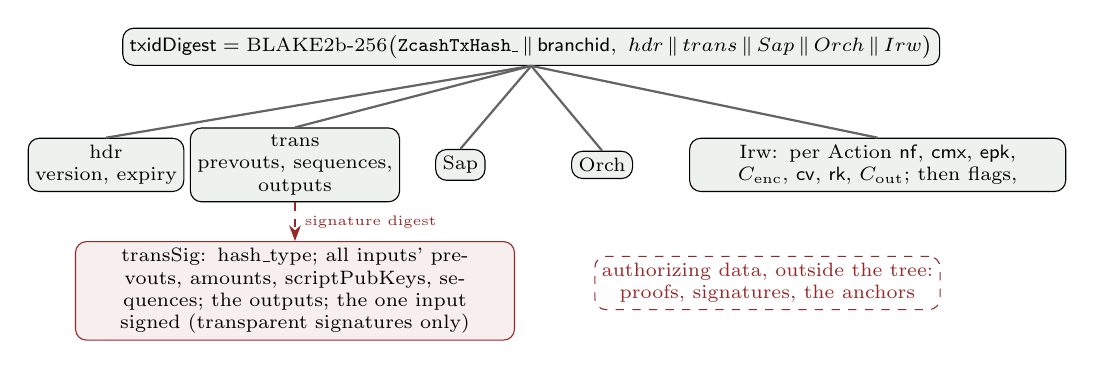
\begin{tikzpicture}[x=1mm,y=1mm,font=\scriptsize,
  nd/.style={draw,rounded corners,inner sep=2.5pt,align=center,fill=arb!8},
  sig/.style={draw,rounded corners,inner sep=2.5pt,align=center,
    fill=arbred!8,draw=arbred},
  auth/.style={draw,dashed,rounded corners,inner sep=2.5pt,align=center,
    draw=arbred,text=arbred},
  e/.style={-,thick,arbdim}]
\node[nd] (root) at (0,0) {$\mathsf{txidDigest} = \mathrm{BLAKE2b}%
  \text{-}256\bigl(\texttt{ZcashTxHash\_}\,\|\,\mathsf{branchid},\
  \wbHd{hdr}\,\|\,\wbHd{trans}\,\|\,\wbHd{Sap}\,\|\,\wbHd{Orch}\,\|\,%
  \wbHd{Irw}\bigr)$};
\node[nd] (hdr) at (-54,-15) {\wbHd{hdr}\\version, expiry};
\node[nd] (tr) at (-30,-15) {\wbHd{trans}\\prevouts, sequences,\\outputs};
\node[nd] (sap) at (-9,-15) {\wbHd{Sap}};
\node[nd] (orch) at (9,-15) {\wbHd{Orch}};
\node[nd,text width=46mm] (irw) at (44,-15) {\wbHd{Irw}: per Action
  $\nfsym$, $\cmx$, $\epk$, $C_{\mathrm{enc}}$, $\cvsym$, $\rksym$,
  $C_{\mathrm{out}}$; then flags, \wbHvbi};
\foreach \c in {hdr,tr,sap,orch,irw} \draw[e] (root.south) -- (\c.north);
\node[sig,text width=54mm] (trs) at (-30,-31) {\wbHd{transSig}:
  hash\_type; all inputs' prevouts, amounts, scriptPubKeys, sequences;
  the outputs; the one input signed (transparent signatures only)};
\draw[-{Stealth[length=2mm]},arbred,dashed] (tr.south) -- (trs.north)
  node[midway,right,font=\tiny,text=arbred]{signature digest};
\node[auth] (au) at (30,-30) {authorizing data, outside the tree:\\
  proofs, signatures, the anchors};
\end{tikzpicture}}\par}
\clearpage
\Write
\begin{itemize}
  \item Every node $=$ one BLAKE2b-256 under its own personalisation; the
    root's carries the branch id
  \item Signature digest $=$ the txid tree with $\wbHd{trans} \to
    \wbHd{transSig}$
  \item No transparent inputs $\Rightarrow$ signature digest $=$ txid
\end{itemize}
\Say
The branch id in the root's personalisation gives the same bytes a
different identity on a parallel chain. Proofs, signatures and the
anchors sit outside the tree, committed through
$\mathsf{hashAuthDataRoot}$ instead.
\end{board}

\begin{board}{What the shielded signatures sign}{authorised}
\Write
\begin{itemize}
  \item Per Action: spend-authorisation signature under \rksym; per
    bundle: binding signature under $\mathsf{bvk}$ --- both sign the
    signature digest: every Action's $\nfsym$, $\cmx$, $\cvsym$,
    $\rksym$, ciphertexts; the flags; \wbHvb
  \item Bitcoin hash\_type: ALL, NONE, SINGLE, each with or without
    ANYONECANPAY: six; a transparent Zcash input: exactly those six
  \item Taproot's SIGHASH\_DEFAULT (a seventh spelling of ALL): not in
    ZIP-244
  \item Shielded: SIGHASH\_ALL, always; no shielded ANYONECANPAY
  \item Anchor: not under the signature from v6; the proof carries it as
    a public input (A3)
  \item Alice: no transparent inputs $\Rightarrow$ $2$ spend-auth $+$ $1$
    binding signature all sign her txid
\end{itemize}
\Say
In Bitcoin each signer picks a hash\_type; a shielded signature has one.
No Action can be transplanted into another transaction, no field
altered. The signature attests to the spend, the proof pins the tree.
\end{board}

\begin{board}{Pools and the doors}{conserved}
{\centering
\resizebox{\textwidth}{!}{%
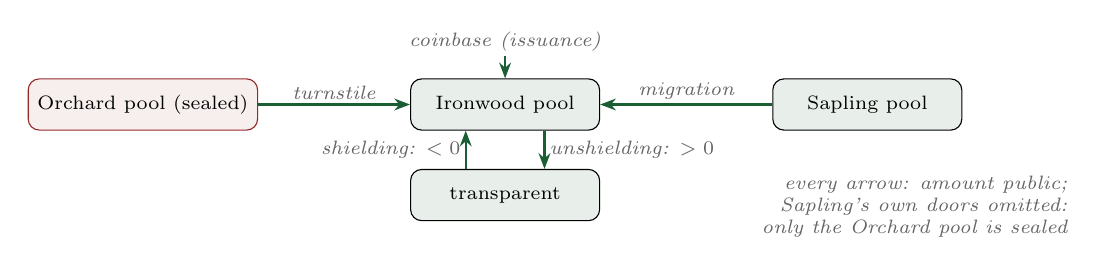
\begin{tikzpicture}[x=1mm,y=1mm,
  pool/.style={draw,rounded corners,minimum width=24mm,minimum height=6.5mm,
    fill=arb!10,font=\scriptsize},
  sealed/.style={pool,fill=arbred!8,draw=arbred},
  flow/.style={-{Stealth[length=2mm]},thick,arb},
  lbl/.style={font=\scriptsize\itshape,text=arbdim,inner sep=1.5pt}]
\node[sealed] (o) at (-46,0) {Orchard pool (sealed)};
\node[pool] (i) at (0,0) {Ironwood pool};
\node[pool] (s) at (46,0) {Sapling pool};
\node[pool] (t) at (0,-11.5) {transparent};
\node[lbl] (cb) at (0,8) {coinbase (issuance)};
\draw[flow] (o) -- (i) node[midway,above,lbl]{turnstile};
\draw[flow] (s) -- (i) node[midway,above,lbl]{migration};
\draw[flow] (cb) -- (i);
\draw[flow] ([xshift=-5mm]t.north) -- ([xshift=-5mm]i.south)
  node[midway,left,lbl]{shielding: $\wbHvb < 0$};
\draw[flow] ([xshift=5mm]i.south) -- ([xshift=5mm]t.north)
  node[midway,right,lbl]{unshielding: $\wbHvb > 0$};
\node[lbl,align=right] at (52,-13) {every arrow: amount public;\\
  Sapling's own doors omitted:\\only the Orchard pool is sealed};
\end{tikzpicture}}\par}
\clearpage
\Write
\begin{itemize}
  \item Shielding: transparent inputs fund $\wbHvbi < 0$; the Actions
    spend dummies, create real notes. Alice shields $10$ ZEC:
    $\wbHvbi = -9.99985$ ZEC printed; her new note not
  \item Coinbase: issuance enters a shielded pool directly; every shielded
    coinbase output decrypts under the all-zero \ovk
  \item Migration: Sapling $\to$ Ironwood; Orchard $\to$ Ironwood through
    the turnstile; both balancing fields cleartext
\end{itemize}
\Say
Bitcoin has one pool and needs no doors. Zcash has several, and value
crosses between them only through doors that print the amount. Wallets
shield automatically, to an internal address.
\end{board}

\begin{board}{The turnstile (ZIP-209): audited at the boundary}{conserved}
\Write
\begin{itemize}
  \item $\mathsf{balance}_{P} := -\sum_{\mathrm{tx}}
    \wbHvb^{P}(\mathrm{tx}) \ge 0$ in every block, for
    $P \in \{\mathsf{Sap}, \mathsf{Orch}, \mathsf{Irw}\}$
  \item Sprout: $\sum \mathtt{vpub\_old} - \sum \mathtt{vpub\_new}$;
    transparent: the UTXO sum; lockbox: its accrued subsidy
  \item A block driving any balance negative, or the total past
    $\mathsf{MAX\_MONEY}$: invalid
  \item Inside a pool: counterfeit undetectable. At the exit: capped at
    what the pool publicly holds
  \item Example: pool holds only Alice's $9.99985$ ZEC; Bob's $+9.99985$
    ZEC exit empties it exactly; one zatoshi more $\Rightarrow$ block
    invalid
\end{itemize}
\Say
Bitcoin audits by summing every coin; inside a shielded pool nothing sums
the notes, and Sprout's original proof system had exactly such a flaw
(Part G). Zcash audits each pool at its door: a forger withdraws at most
what the pool publicly holds. The Sapling pool still rests on its Groth16
ceremony; the turnstile bounds it.
\end{board}

\begin{board}{Why the Orchard pool is sealed}{conserved}
\Write
\begin{itemize}
  \item Three rules: no issuance; no circulation
    ($\mathsf{enableCrossAddress} = 0$);\newline no entry ($\wbHvbo \ge 0$)
    --- whatever the transaction version
  \item Legacy note, lead byte $\mathtt{0x02}$: not quantum-recoverable.
    Ironwood note, lead byte $\mathtt{0x03}$, hashed \rcm: recoverable
  \item Orchard pool balance can only fall; every exit metered in
    cleartext by \wbHvbo
  \item Bitcoin never retires an output type; a P2PK coin spends forever
\end{itemize}
\Say
The seal is the three rules of Parts C and E; the reason is Part F's one
note-level difference. Consensus stops the old notes circulating and
funnels their value out through the turnstile, while owners can still
spend what they hold. The turnstile is the seal's accounting shape.
\end{board}

\begin{board}{Fees (ZIP-317): a function of the public shape}{conserved}
\Write
\begin{align*}
  \mathit{fee} &= 5000 \cdot \max(2,\ \mathit{logical\_actions})
  \quad\text{zatoshi} \\[2pt]
  \mathit{logical\_actions} &=
  \max\Bigl(\Bigl\lceil \tfrac{\text{in bytes}}{150} \Bigr\rceil,
            \Bigl\lceil \tfrac{\text{out bytes}}{34} \Bigr\rceil\Bigr)
  + 2\,\mathit{nJoinSplit}_{\mathrm{Sprout}} \\
  &\quad + \max(\mathit{spends}, \mathit{outputs})_{\mathrm{Sap}}
  + \mathit{nActions}_{\mathrm{Orch}}
  + \mathit{nActions}_{\mathrm{Irw}}
\end{align*}
\begin{itemize}
  \item Divisors: standard P2PKH input $150$~B, output $34$~B
  \item Alice: two Actions, $5000 \cdot \max(2, 2) = 10\,000$ zatoshi
  \item One Action padded to two: $10\,000$, the same
  \item Shielding with one P2PKH input: $1 + 2 = 3$ actions, $15\,000$
\end{itemize}
\Say
Bitcoin reads the fee by subtraction; here the amounts are hidden, so the
fee is a function of the public shape. An Action spends one note and
creates one, so it is counted once.
\end{board}

\begin{board}{Fees (ZIP-317): why a convention, and who enforces
  it}{conserved}
\Write
\begin{itemize}
  \item Computable from public fields alone
  \item Uniform across wallets: not a fingerprint; padding to two is free
    (grace window $= 2$)
  \item A convention, not consensus: relay at least the fee; template by
    fee ratio, capped at $4\times$; at most $50$ unpaid actions per block
  \item Bitcoin: a market --- bid per virtual byte and coin selection
    vary; both fingerprints
\end{itemize}
\Say
Bitcoin's fee market is read as a fingerprint; Zcash flattens the market
on purpose. A fee that depended on which notes were spent or what change
came back would print that data in the amount paid. Overpaying beyond
$4\times$ buys no further priority.
\end{board}

\begin{board}{The public face of Alice's transaction}{all four}
{\centering\small\setlength{\tabcolsep}{4pt}
\begin{tabular}{@{}p{34mm}p{106mm}@{}}
\toprule
\textbf{public field} & \textbf{Alice pays Bob $1.5$ ZEC from a $2$ ZEC
  note} \\
\midrule
version & v6; transparent, Sapling and Orchard parts empty \\
Ironwood Actions & $2$ (one real spend, one dummy; shuffled) \\
nullifiers, \mbox{commitments} & $2$ and $2$ \\
\wbHvbi{} & $+10\,000$ zatoshi $=$ the fee \\
anchor & the Ironwood root at the newest shared checkpoint at or below
  $H - 3$ \\
expiry & target height $+\,40$ blocks, about $50$ minutes \\
signatures & $2$ spend-authorisation $+$ $1$ binding \\
size & $9166$ bytes, $7264$ of them proof \\
\bottomrule
\end{tabular}\par}
\Write
\begin{itemize}
  \item Bitcoin prints: input coin, both amounts, both scripts, fee by
    subtraction
  \item Here printed: the fee alone, as \wbHvbi
  \item Inside the commitments: $2$ ZEC, $1.5$ ZEC, $0.4999$ ZEC change,
    both addresses
\end{itemize}
\end{board}

\begin{board}{The privacy sliders: pool, address type, timing}{all four}
\Write
\begin{itemize}
  \item Pool: transparent leg prints its amount as \wbHvb; fully shielded
    prints the fee and nothing else
  \item Address type: unified address $=$ bundle of receivers; wallet
    MUST use the most preferred it supports: Orchard-protocol (Ironwood
    pool) $>$ Sapling $>$ transparent. TEX address $\Rightarrow$ two
    transactions via an ephemeral transparent output, both public
  \item Timing: expiry $=$ target $+\,40$ blocks, wallets SHOULD keep it.
    Migration: denominations $m \cdot 10^{k}$ ZEC, $m \in \{1, 2, 5\}$;
    anchors and expiries from shared grids
  \item ``Uniformity is the strategy''
\end{itemize}
\Say
Bitcoin has the address-type and timing sliders but no pool slider: one
plaintext ledger. An idiosyncratic expiry delta fingerprints a
transaction as an idiosyncratic fee would. The defaults protect only
while everyone keeps them.
\end{board}

\begin{board}{PSBT $\to$ PCZT (ZIP-374): the unfinished
  transaction}{authorised}
\Write
\begin{itemize}
  \item PSBT (BIP-174 $+$ BIP-370): Creator, Constructor, Updater, Signer,
    Combiner, Input Finalizer, Transaction Extractor
  \item PSBT cannot carry shielded: no shielded spends/outputs; no proof
    distinct from a signature; tolerates unknown fields
  \item PCZT $=$ PSBT roles $+$ IO Finalizer, Redactor, Prover; ten roles
  \item ``Proving is delegated, signing is not''
\end{itemize}
\Say
Hardware wallets and multisig live on PSBT. The IO Finalizer declares the
inputs and outputs complete and derives the binding-signature key; the
Redactor strips what later parties need not see. The Prover has no PSBT
counterpart: a hardware signer cannot compute a Halo 2 proof, and a proof
needs no spending key. Signers can be fully offline.
\end{board}

\begin{board}{Signer versus Prover}{authorised}
{\centering\setlength{\tabcolsep}{4pt}
\begin{tabular}{@{}p{26mm}p{57mm}p{57mm}@{}}
\toprule
 & \textbf{Signer} & \textbf{Prover} \\
\midrule
holds & \asksym{}, spend authority & \fvk{}, no spending key \\
reads from the PCZT & $\alpha$, \rksym; the spend's public fields and,
  unless redacted, its note fields & the note ($\gd$, $\pkd$, $v$,
  $\rho$, $\mathsf{rseed}$), the witness, $\alpha$, \rcv, the anchor \\
computes & the sighash from the effecting data; $\rsk = \asksym +
  \alpha$, checks it matches \rksym, signs & one Halo 2 proof over all
  Actions; anchor and flags as public inputs \\
verifies first & $\nfsym$, $\cvsym$, $\cmx$ against the note fields:
  exactly what it authorises & \fvk{} owns each note;
  $\rho_{\mathrm{new}} = \nfsym_{\mathrm{old}}$ \\
learns & what it signs & the notes' private data,\newline not authority \\
\bottomrule
\end{tabular}\par}
\clearpage
\Write
\begin{itemize}
  \item $\rsk = \asksym + \alpha$; check against \rksym{} before signing
  \item $\rho_{\mathrm{new}} = \nfsym_{\mathrm{old}}$
  \item Either role runs without the other; the Prover never sees
    \asksym; the Signer may see the note data, or have it redacted
\end{itemize}
\Say
In Bitcoin there is no proof distinct from the signature, so the signer
is the only role that attests. Here proof and signature are separate
artefacts with separate secrets.
\end{board}

\begin{board}{PCZT: where it stands}{authorised}
\Write
\begin{itemize}
  \item From v6: signatures commit to no anchor $\Rightarrow$ sign today,
    anchor, witness and prove at broadcast
  \item Delegating the Prover reveals note data, never spend authority;
    a Redactor strips what a later party need not see
  \item Bins: ZIP Draft; format released as a library; deployed wallet
    pipeline drives the roles end to end (Ironwood sent-output records
    not yet stored: backend gap)
  \item $+$ FROST (Part I): ``no script, so no multisig and no hardware
    wallets'' --- closed
\end{itemize}
\Ask
Alice shields $10$ ZEC; the next day Bob unshields $9.9997$ ZEC. What can
a chain analyst conclude, and what can they not?
\Answer
\begin{itemize}
  \item \textbf{Conclude.} Two cleartext balancing fields, exact to the
    zatoshi: $-9.99985$ ZEC entered, $+9.99985$ ZEC left --- $10$ ZEC
    less two conventional fees of $15\,000$ zatoshi; the heights; the
    transparent addresses on each side; that the amounts match exactly
    and the times are close.
  \item \textbf{Not conclude.} That Bob's coins were Alice's. Her
    commitment hides her note; his nullifier is keyed by his \nksym; his
    candidate set is every leaf under his anchor. Her note may still be
    resting.
\end{itemize}
Bitcoin would have handed over the path; Zcash hands over a correlation.
Canonical denominations and shared timing grids exist because that
correlation is evidence.
\end{board}

%% ---- 10-consensus.tex
%% Screen version, Part K --- Consensus. Source: wb/10-consensus.tex.

\section{Part K --- Consensus: why one fork wins, and what the chain
  must remember}

\begin{board}{Bitcoin's chain rule, weighed in work}{not twice}
\centerline{\resizebox{0.7\textwidth}{!}{%
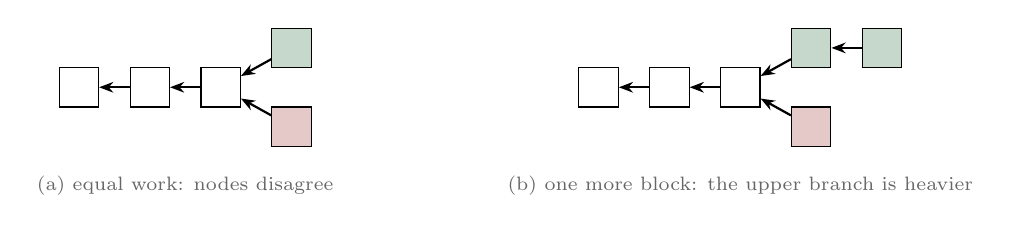
\begin{tikzpicture}[
  blk/.style={draw, rectangle, minimum width=5mm, minimum height=5mm,
    inner sep=0pt, fill=white},
  hon/.style={blk, fill=arb!25},
  att/.style={blk, fill=arbred!25},
  lnk/.style={-{Stealth[length=1.8mm]}, thick},
  lbl/.style={font=\scriptsize, text=black!60},
]
\begin{scope}
\node[blk] (g) at (0,0) {};
\node[blk] (b1) at (0.9,0) {};
\node[blk] (b2) at (1.8,0) {};
\node[hon] (c1) at (2.7,0.5) {};
\node[att] (d1) at (2.7,-0.5) {};
\draw[lnk] (b1) -- (g); \draw[lnk] (b2) -- (b1);
\draw[lnk] (c1) -- (b2); \draw[lnk] (d1) -- (b2);
\node[lbl, anchor=north] at (1.35,-1.0) {(a) equal work: nodes disagree};
\end{scope}
\begin{scope}[xshift=6.6cm]
\node[blk] (g) at (0,0) {};
\node[blk] (b1) at (0.9,0) {};
\node[blk] (b2) at (1.8,0) {};
\node[hon] (c1) at (2.7,0.5) {};
\node[hon] (c2) at (3.6,0.5) {};
\node[att] (d1) at (2.7,-0.5) {};
\draw[lnk] (b1) -- (g); \draw[lnk] (b2) -- (b1);
\draw[lnk] (c1) -- (b2); \draw[lnk] (c2) -- (c1); \draw[lnk] (d1) -- (b2);
\node[lbl, anchor=north] at (1.8,-1.0) {(b) one more block: the upper
  branch is heavier};
\end{scope}
\end{tikzpicture}}}
\Write
\begin{itemize}
  \item work of a block $= \lfloor 2^{256} /
    (\mathsf{ToTarget}(\mathtt{nBits}) + 1) \rfloor$
  \item best valid chain $=$ greatest total work; ties $\to$ the block
    received first
  \item ``longest'' $=$ ``most work'' only at constant difficulty
  \item nothing marks a chain as final
\end{itemize}
\Say
Every block names its parent, so the node holds a tree of blocks; each
branch is one consistent history, and sibling branches may conflict. A
heavier branch wins however deep the fork.
\end{board}

\begin{board}{Two double-spends; consensus answers one}{not twice}
\Write
\begin{itemize}
  \item same chain: two spends of one note $\Rightarrow$ the same
    $\nfsym$ twice $\Rightarrow$ invalid by rule; no race, no
    probability
  \item chain level: pay on the chain everyone sees, then replace that
    chain; no proof rules it out, only the proof-of-work race bounds it
  \item Bitcoin: the same two attacks; a UTXO lookup there, a nullifier
    lookup here
\end{itemize}
\Say
Bitcoin stops a double spend in two places: a UTXO lookup on the chain
it holds, and the work rule between chains. Both attacks exist here;
the first changes shape and the second does not. The second is what
this part measures.
\end{board}

\begin{board}{The attack}{not twice}
\Write
\begin{enumerate}
  \item broadcast the payment to the merchant
  \item mine a secret branch from the last pre-payment block, carrying a
    conflicting payment to yourself
  \item wait until the merchant ships at $n$ confirmations
  \item extend the secret branch until it carries more work, then
    release it
\end{enumerate}
\medskip
step 4 breaks no validity rule --- does the secret branch ever get
ahead?
\Say
Bitcoin's whitepaper analyses this attack in its \S11, approximately;
Rosenfeld's \emph{Analysis of hashrate-based double-spending} is the
exact counterpart, and this part follows it throughout. The released
branch is a well-formed chain, merely a different one; the only
question is probabilistic, and from here on its odds are computed
exactly.
\end{board}

\begin{board}{The model: memoryless clocks}{not twice}
\Write
\begin{itemize}
  \item $\Pr[X > t] = e^{-\lambda t}$; \quad
    $\Pr[X > s + t \mid X > s] = \Pr[X > t]$
  \item two clocks: $\Pr[X < Y] = \lambda / (\lambda + \mu)$; the winner
    is independent of the winning time
  \item honest rate $p / T_0$, attacker rate $q / T_0$, $p + q = 1$;
    both restart at every block
  \item next block is the attacker's with probability $q$, independently
    of everything before
  \item block attribution $=$ an i.i.d.\ $p/q$ coin sequence; $T_0$
    drops out of every answer
\end{itemize}
\Say
This is Rosenfeld's version of the whitepaper's race between an honest
and an attacking hashrate, with its two assumptions explicit: constant
hashrates and constant difficulty. An exponential clock of rate
$\lambda$ is memoryless: having waited $s$ says nothing about the wait
still to come. Here $T_0$ is the network's mean block time. How well
Equihash fits the model is a deployment question (later in this part).
\end{board}

\begin{board}{The negative binomial law}{not twice}
\Write
\begin{itemize}
  \item $m =$ attacker blocks found strictly before the honest network's
    $n$-th block
  \item $P(m) = \binom{m + n - 1}{m}\, p^{n} q^{m}$, \quad
    $m = 0, 1, 2, \ldots$
  \item first-to-$n$ race: $H_n$ or $A_n$; no tie;
    $\Pr[H_n] + \Pr[A_n] = 1$
  \item $q = 1/5$, $n = 6$: $P(0) = 0.262144$, $P(1) = 0.314573$,
    $P(2) = 0.220201$, \dots, $P(5) = 0.021139$;
    $\Pr[m \geq 6] = 0.011654$
\end{itemize}
\Say
Bitcoin's whitepaper approximates the attacker's progress by a Poisson;
this is the exact law. The $(m+n)$-th trial is the $n$-th honest
success, and the $m$ attacker blocks sit among the first $m + n - 1$
trials in any order. Counts advance one at a time, so the first-to-$n$
race has no tie. The running numbers return in the worked race.
\end{board}

\begin{board}{The catch-up theorem (Rosenfeld \S3)}{not twice}
\Write
\begin{itemize}
  \item $z =$ the honest lead in blocks; up $1$ with probability $p$,
    down $1$ with probability $q$; success $=$ $z$ reaches $-1$
    (strictly ahead)
\end{itemize}
\[
  a_z \;=\; \Pr[\text{walk from } z \text{ ever reaches } -1]
  \;=\;
  \begin{cases}
    1 & z < 0 \text{ or } q \geq p,\\[2pt]
    (q/p)^{\,z+1} & z \geq 0 \text{ and } q < p.
  \end{cases}
\]
\begin{itemize}
  \item each block of deficit multiplies the chance by $q/p$
  \item $q \geq p$: overtake with probability $1$ from any finite
    deficit
  \item whitepaper: $(q/p)^{z}$ --- breakeven scoring, no pre-mined
    block
\end{itemize}
\Say
Bitcoin's whitepaper asks how an attacker $z$ blocks behind ever catches
up; Rosenfeld answers exactly. Two forks cannot compete for long: one
quickly wins. At $q \geq p$ no confirmation count defends. The two
conventions cancel term for term (confirmations boards).
\end{board}

\begin{board}{Proof idea: a walk between two barriers}{not twice}
\Write
\begin{gather*}
  h_N(z) = p\, h_N(z+1) + q\, h_N(z-1), \qquad
  h_N(-1) = 1,\quad h_N(N) = 0 \\
  p\,t^{2} - t + q \;=\; p\,(t - 1)\,(t - q/p) \\
  q \neq p:\quad
  h_N(z) \;=\; \frac{(q/p)^{z} - (q/p)^{N}}{(q/p)^{-1} - (q/p)^{N}}
  \;\xrightarrow{\;N \to \infty\;}\;
  \begin{cases}
    (q/p)^{\,z+1} & q < p,\\
    1 & q > p,
  \end{cases} \\
  q = p:\quad h_N(z) = (N - z)/(N + 1) \to 1
\end{gather*}
\Say
Absorb the walk at $-1$ and at a far barrier $N > z$; $h_N(z)$ is the
chance of reaching $-1$ first, conditioned on the first step. The trial
$t^{z}$ solves the recurrence exactly when $t$ is a root of
$p t^{2} - t + q$; the two boundary values then fix $h_N(z)$. The limit
is legitimate because the events ``reach $-1$ before $N$'' increase to
``ever reach $-1$''.
\end{board}

\begin{board}{The deficit walk}{not twice}
\centerline{\resizebox{!}{0.42\textheight}{%
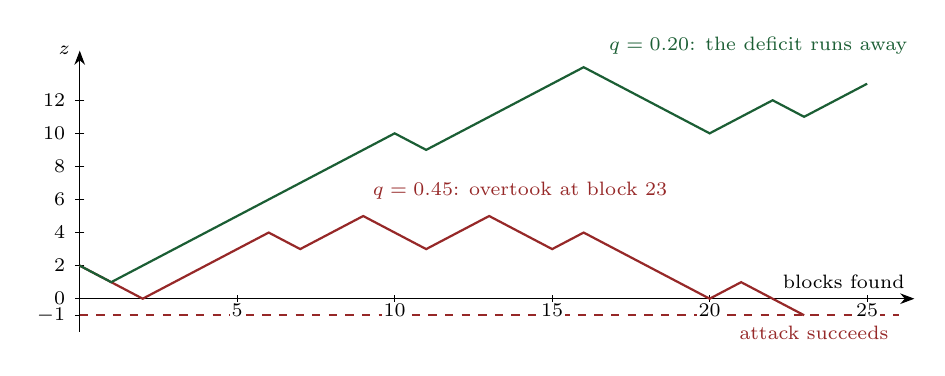
\begin{tikzpicture}[x=0.40cm, y=0.21cm]
\draw[-{Stealth[length=1.8mm]}] (0,-2) -- (0,15)
  node[left, font=\scriptsize] {$z$};
\draw[-{Stealth[length=1.8mm]}] (0,0) -- (26.5,0)
  node[above left, font=\scriptsize] {blocks found};
\foreach \y in {-1, 0, 2, 4, 6, 8, 10, 12}
  \draw (0.15,\y) -- (-0.15,\y) node[left, font=\scriptsize] {$\y$};
\draw[dashed, thick, arbred] (0,-1) -- (26,-1)
  node[below left, font=\scriptsize, text=arbred] {attack succeeds};
\foreach \x in {5, 10, 15, 20, 25}
  \draw (\x,0.2) -- (\x,-0.2) node[below, font=\scriptsize, fill=white,
    inner sep=0.6pt] {$\x$};
\draw[thick, arbred] plot coordinates {(0,2) (1,1) (2,0) (3,1) (4,2)
  (5,3) (6,4) (7,3) (8,4) (9,5) (10,4) (11,3) (12,4) (13,5) (14,4)
  (15,3) (16,4) (17,3) (18,2) (19,1) (20,0) (21,1) (22,0) (23,-1)};
\node[font=\scriptsize, text=arbred, anchor=south west] at (9,5.4)
  {$q = 0.45$: overtook at block $23$};
\draw[thick, arb] plot coordinates {(0,2) (1,1) (2,2) (3,3) (4,4) (5,5)
  (6,6) (7,7) (8,8) (9,9) (10,10) (11,9) (12,10) (13,11) (14,12) (15,13)
  (16,14) (17,13) (18,12) (19,11) (20,10) (21,11) (22,12) (23,11)
  (24,12) (25,13)};
\node[font=\scriptsize, text=arb, anchor=south west] at (16.5,14.2)
  {$q = 0.20$: the deficit runs away};
\end{tikzpicture}}}
\Write
\begin{itemize}
  \item from deficit $13$ at $q = 0.20$: $(1/4)^{14} \approx 3.7 \times
    10^{-9}$
  \item $q = 10\%$: $a_0 = 1/9 \approx 0.1111$, \quad $a_5 \approx 1.88
    \times 10^{-6}$
  \item $q = 30\%$: $a_0 = 3/7 \approx 0.4286$, \quad $a_5 \approx 6.20
    \times 10^{-3}$
\end{itemize}
\Say
Two seeded runs from $z = 2$ show the theorem in motion.
\end{board}

\begin{board}{Waiting for confirmations: the pre-mined block}{not twice}
\Write
\begin{itemize}
  \item the merchant ships after $n$ confirmations; one attacker block
    banked before scoring; $m$ further attacker blocks
  \item $z = n - m - 1$
\end{itemize}
\[
  r(q, n)
  \;=\; \underbrace{\sum_{m=0}^{n-1} P(m)\,(q/p)^{\,n-m}}_{
    \text{behind: must catch up}}
  \;+\; \underbrace{\sum_{m \geq n} P(m)}_{\text{already ahead}}
\]
\begin{itemize}
  \item $r = 1$ when $q \geq p$ (every catch-up factor is $1$)
  \item no banked block: walk starts at $n - m$, every probability
    shrinks
\end{itemize}
\Say
Rosenfeld banks one attacker block before the race is scored. Average
the catch-up probability over the negative binomial $m$: behind for
$m \leq n - 1$, already ahead for $m \geq n$. The banked block is a
modelling choice.
\end{board}

\begin{board}{Rosenfeld eq.~(1): the closed forms}{not twice}
\setlength{\abovedisplayskip}{3pt}\setlength{\belowdisplayskip}{3pt}
\setlength{\jot}{0pt}
\Write
\begin{gather*}
  \binom{m+n-1}{m}\, p^{n} q^{m} \left( \frac{q}{p} \right)^{\!n-m}
  \;=\; \binom{m+n-1}{m}\, p^{m} q^{n} \\
  r(q, n)
  \;=\; 1 - \sum_{m=0}^{n-1} \binom{m+n-1}{m}
        \bigl( p^{n} q^{m} - p^{m} q^{n} \bigr) \\
  \;=\; 2 \sum_{m=0}^{n-1} \binom{m+n-1}{m} p^{m} q^{n}
  \;=\; 2 \Pr[A_n]
\end{gather*}
race doubling: catch-up half $=$ already-ahead half
\Say
Each catch-up term transforms into the probability that the attacker's
$n$-th block arrives while the honest side holds $m$; summed, this is
$\Pr[A_n]$, as is the already-ahead tail.
\end{board}

\begin{board}{A full race, exactly: $q = 1/5$, $n = 6$}{not twice}
\Write
\noindent\begin{minipage}[t]{0.5\textwidth}
\small
\begin{tabular}[t]{@{}rrrr@{}}
\toprule
$m$ & $P(m)$ & $a_{5-m} = 4^{-(6-m)}$ & product \\
\midrule
$0$ & $0.262144$ & $0.000244$ & $0.000064$ \\
$1$ & $0.314573$ & $0.000977$ & $0.000307$ \\
$2$ & $0.220201$ & $0.003906$ & $0.000860$ \\
$3$ & $0.117441$ & $0.015625$ & $0.001835$ \\
$4$ & $0.052848$ & $0.062500$ & $0.003303$ \\
$5$ & $0.021139$ & $0.250000$ & $0.005285$ \\
\midrule
\multicolumn{3}{@{}l}{catch-up half} & $0.011654$ \\
\multicolumn{3}{@{}l}{already-ahead half, $\Pr[m \geq 6]$} & $0.011654$ \\
\multicolumn{3}{@{}l}{$r(1/5,\, 6)$} & $0.023308$ \\
\bottomrule
\end{tabular}
\end{minipage}\hfill
\begin{minipage}[t]{0.46\textwidth}
\raggedright
\begin{itemize}
  \item deficit starts at $z = 5 - m$; catch-up factor $4^{-(6-m)}$
  \item the halves agree to every digit; closed form gives the same
    $0.023308$
  \item six confirmations, $20\%$ adversary: $2.33\%$ strict-overtake
    risk
\end{itemize}
\Say
Six confirmations is Bitcoin's folk number; here is what it buys,
exactly. Every entry is an exact rational, printed to six decimals.
\end{minipage}
\end{board}

\begin{board}{Satoshi's approximation}{not twice}
\centerline{\begin{tabular}{@{}rrrr@{}}
\toprule
$q$ & $n$ & whitepaper & exact \\
\midrule
$10\%$ & $6$ & $0.0243\%$ & $0.0591\%$ \\
$30\%$ & $6$ & $13.211\%$ & $15.645\%$ \\
$10\%$ & $10$ & $0.0001\%$ & $0.0008\%$ \\
\bottomrule
\end{tabular}}
\Write
\begin{itemize}
  \item Poisson, mean $\lambda = nq/p$: $\Pr[k] = e^{-\lambda}
    \lambda^{k} / k!$
  \item no pre-mined block, success at breakeven: catch-up factor again
    $(q/p)^{n-m}$, term for term
  \item the conventions cancel; the Poisson step is the entire gap
\end{itemize}
\Say
The whitepaper computes the same quantity with one approximation and
two offsetting conventions. In each pair the approximation understates
the risk; the direction is not uniform over all $(q, n)$.
\end{board}

\begin{board}{Blocks, not time}{not twice}
\Write
\begin{itemize}
  \item $r(q, n)$ contains no $T_0$: security per confirmation depends
    on block counts alone
  \item Zcash $75$-second blocks; Bitcoin $600$
  \item thirty minutes $= 3$ Bitcoin or $24$ Zcash confirmations
    (nominal); under a $10\%$ attack either wait $\approx 33.3$ min
    (public blocks arrive at rate $p$)
  \item $r(0.1, 3) = 1.712\%$ \quad versus \quad $r(0.1, 24) \approx
    3.2 \times 10^{-12}$
  \item caveat: no network in the model; faster blocks raise honest
    self-orphaning, which effectively raises $q$
\end{itemize}
\Say
Two chains with the same $q$ offer identical security per confirmation,
and therefore different security per minute. At $q = 10\%$ the same
nominal wait differs by nine orders of magnitude; ZIP-208 makes this
argument for the spacing. The comparison holds $q$ fixed.
\end{board}

\begin{board}{What the numbers say: $r(q, n)$ in percent}{not twice}
\Write
\noindent\begin{minipage}[t]{0.5\textwidth}
\small
\begin{tabular}[t]{@{}rrrrr@{}}
\toprule
$q$ & $n{=}1$ & {\color{arb}$\mathbf{n{=}3}$} & $n{=}6$
  & {\color{arb}$\mathbf{n{=}10}$} \\
\midrule
$2\%$ & $4.000$ & $0.016$ & $5.4\cdot10^{-6}$ & $1.6\cdot10^{-10}$ \\
$5\%$ & $10.000$ & $0.232$ & $0.0012$ & $1.2\cdot10^{-6}$ \\
$10\%$ & $20.000$ & $1.712$ & $0.059$ & $0.0008$ \\
$20\%$ & $40.000$ & $11.584$ & $2.331$ & $0.316$ \\
$30\%$ & $60.000$ & $32.616$ & $15.645$ & $6.511$ \\
$40\%$ & $80.000$ & $63.488$ & $49.300$ & $37.218$ \\
$45\%$ & $90.000$ & $81.375$ & $73.375$ & $65.793$ \\
$50\%$ & \multicolumn{4}{l}{$100$ for every $n$} \\
\bottomrule
\end{tabular}
\end{minipage}\hfill
\begin{minipage}[t]{0.48\textwidth}
\raggedright
\begin{itemize}
  \item columns $n = 3$ and $n = 10$: deployed wallet defaults, $3$
    trusted / $10$ untrusted
  \item $10\%$ adversary: $1.712\%$ at three, $0.0008\%$ at ten; $20\%$
    adversary: $0.316\%$ at ten
  \item every fixed count $=$ a $(q, \varepsilon)$ policy
\end{itemize}
\Say
Bitcoin's six assumes an attacker below $10\%$ and a tolerable risk
below $0.1\%$; both figures are arbitrary. Every fixed count is an
assumed adversary and an accepted risk, not a law of nature.
\end{minipage}
\end{board}

\begin{board}{Pick the adversary and the risk; read off $n$}{not twice}
\Write
\noindent\begin{minipage}[t]{0.44\textwidth}
\begin{tabular}[t]{@{}rrrr@{}}
\toprule
$q$ & $r < 10\%$ & $r < 1\%$ & $r < 0.1\%$ \\
\midrule
$5\%$ & $2$ & $3$ & $4$ \\
$10\%$ & $2$ & $4$ & $6$ \\
$20\%$ & $4$ & $8$ & $13$ \\
$30\%$ & $9$ & $20$ & $32$ \\
$40\%$ & $34$ & $82$ & $133$ \\
$45\%$ & $135$ & $331$ & $539$ \\
\bottomrule
\end{tabular}
\end{minipage}\hfill
\begin{minipage}[t]{0.53\textwidth}
\raggedright
\begin{itemize}
  \item least $n$ with $r(q, n)$ below target: logarithmic in the
    inverse risk, explosive in $q$
  \item $10\%$ attacker $\to$ $6$ confirmations; $45\%$ attacker $\to$
    $539$ ($\approx 11.2$ h of Zcash blocks)
  \item no finite count is final: $r(q, n) \geq 2q^{n} > 0$
  \item $r(1/2, n) = 1$ for every $n$: required $n \to \infty$ as
    $q \uparrow 1/2$
\end{itemize}
\end{minipage}
\Say
The attacker may simply find the first $n$ blocks, so no finite count
is final. Bitcoin: the same table; only the wall-clock price of a row
differs.
\end{board}

\begin{board}{The economics: when the attack pays}{not twice}
\Write
\begin{itemize}
  \item $k$ merchants at $v$ each; goods worth $\alpha v$ to the
    attacker; give up after $o$ vain blocks; block income $B$
\end{itemize}
\begin{gather*}
  k\alpha v - (1 - r)(kv + oB)
  \;=\; kv(\alpha + r - 1) - (1 - r)\,oB \\
  v \;\leq\; \frac{o\,(1 - r)\,B}{k\,(\alpha + r - 1)}
  \;\overset{\alpha = 1}{=}\;
  \frac{o}{k} \cdot \frac{B\,(1 - r)}{r}
\end{gather*}
\begin{itemize}
  \item subsidy $1.5625$ ZEC; funding streams take $20\%$; miner's
    $B = 1.25$ ZEC $+$ fees
  \item Bitcoin (Rosenfeld): $B = 25$ BTC, $o = 20$, $k = 5$,
    $\alpha = 1$: $v \leq 100\,(1/r - 1)$ BTC; here
    $\lfloor 4B(1 - r)/r \rfloor$
\end{itemize}
\Say
Rosenfeld's profitability question is Bitcoin's; only the cost unit
changes. The first line is the expected profit over not attacking; it
is non-positive whenever $v$ is at most the bound. Fees raise $B$, and
the threshold, linearly.
\end{board}

\begin{board}{The largest payment the modelled attack cannot profit
  from}{not twice}
\centerline{\small
\begin{tabular}{@{}rrrrrrr@{}}
\toprule
$q$ & $n{=}1$ & $2$ & $4$ & $6$ & $8$ & $10$ \\
\midrule
$5\%$ & $45$ & $339$ & $12{,}909$ & $430{,}929$ & $13{,}664{,}382$
  & $420{,}922{,}251$ \\
$10\%$ & $20$ & $84$ & $911$ & $8{,}449$ & $74{,}344$ & $636{,}146$ \\
$20\%$ & $7$ & $19$ & $69$ & $209$ & $584$ & $1{,}578$ \\
$30\%$ & $3$ & $6$ & $14$ & $26$ & $44$ & $71$ \\
$40\%$ & $1$ & $2$ & $3$ & $5$ & $6$ & $8$ \\
\bottomrule
\end{tabular}}
\Write
\begin{itemize}
  \item whole ZEC: $\lfloor 4B(1 - r)/r \rfloor$, $B = 1.25$ ZEC
  \item heuristic: unlimited-horizon $r(q, n)$ stands in for the
    $o = 20$ stopping rule
  \item $30\%$ attacker, six confirmations: unprofitable only up to
    about $26$ ZEC
\end{itemize}
\Say
Rosenfeld's Table 2 with $B = 1.25$ ZEC in place of $25$ BTC: patience
buys safety exponentially.
\end{board}

\begin{board}{Majority is a different problem}{not twice}
\Write
\begin{itemize}
  \item $q = p$: strict overtake certain, zero drift, no lasting
    monopoly
  \item $q > p$: double-spend at no cost beyond normal mining; reject
    every other miner's blocks; exclude transactions at will
  \item confirmation policy is not the defence; the cost of assembling
    the majority is, and it lies outside this model
\end{itemize}
\Say
Past $q = p$ the attacker takes the whole issuance and excludes
transactions at will --- an attempt to destroy the currency, motivated
from outside it. Rosenfeld's remark is about Bitcoin; nothing in it
depends on the chain.
\end{board}

\begin{board}{Deployed rails}{not twice}
\small\setlength{\tabcolsep}{4pt}
\begin{tabular}{@{}lll@{}}
\toprule
Rail & Value & Standing \\
\midrule
reorg window & $1000$ blocks ($\approx 20.8$ h)
  & \parbox[t]{26mm}{\raggedright Zebra policy; the spec says $100$} \\
coinbase maturity & $100$ blocks ($125$ min), transparent & consensus \\
difficulty & every block; window $17$, damping $4$, clamp $16\%$/$32\%$
  & consensus \\
proof of work & Equihash $(200, 9)$, SHA-256d filter & consensus \\
wallet waits & $3$ trusted / $10$ untrusted; anchor $\leq H - 3$
  & wallet policy \\
\bottomrule
\end{tabular}
\Write
\begin{itemize}
  \item miners wait $n = 100$: $r(0.3, 100) \approx 3.7 \times
    10^{-9}$, \; $r(0.4, 100) \approx 0.43\%$, \; $r(0.45, 100) \approx
    15.7\%$
  \item the window caps automatic rollback, not the theory
\end{itemize}
\Say
Bitcoin inherits coinbase maturity and the memoryless race; per-block
retargeting and the block spacing it does not.
\end{board}

\begin{board}{Where the deployed rule departs from the model}{not twice}
\Write
\begin{itemize}
  \item tie-break: specification and Rosenfeld $=$ first seen; Zebra
    $=$ the larger tip hash (no arrival times tracked)
  \item $r(q, n)$: exact for the strict-overtake model; a lower bound
    if only the tie-break is replaced by Zebra's; not a bound on the
    full deployed process
  \item Equihash: each candidate solution $=$ a fresh SHA-256d lottery;
    headers are the model's Bernoulli trials; granularity per solver
    run against $75$-second spacing
\end{itemize}
\Say
Bitcoin's nodes keep the first-seen rule; the deployed Zcash node does
not. Zebra downloads blocks in parallel and tracks no arrival times, so
it prefers the larger tip hash. At equal work an attacker whose private
tip hash wins may reveal at once; the strict-overtake boundary $z = -1$
does not count that success. The exponential clock is good only while
a solver run is short against the spacing; Bitcoin's hash trials are
the model's ideal.
\end{board}

\begin{board}{What consensus adds for shielded state: the nullifier
  set}{not twice}
\Write
\begin{itemize}
  \item ``A nullifier MUST NOT repeat either within a transaction, or
    across transactions in a valid block chain.''
  \item pools' nullifiers ``considered disjoint, even if they have the
    same bit pattern''
  \item in block order, per transaction: check $\nfsym_{\mathrm{old}}
    \notin$ set $\;\to\;$ record $\nfsym_{\mathrm{old}}$ $\;\to\;$
    append $\cmx_{\mathrm{new}}$
  \item the one check that cannot sit inside a proof
  \item sets per pool (ZIP-229): $\rho_{\mathrm{new}} :=
    \nfsym_{\mathrm{old}}$ unique pool-locally, not globally
\end{itemize}
\Say
In Bitcoin the node looks the outpoint up in the UTXO set, an ordered,
stateful check against the whole history. Here the note is never named,
so the node checks a serial number instead. The next spender proves
membership against the new root; a second spend of the same note
fails. The check concerns the global history, not one transaction.
\end{board}

\begin{board}{Anchors, balances, and no mempool chains}{exists,
  conserved}
\Write
\begin{itemize}
  \item anchor ``MUST refer to some earlier block's final'' treestate of
    its pool; never mid-block; any main-chain block since the pool's
    activation; $H - 3$ is wallet policy
  \item no spend of an unmined note: not an output of its own
    transaction; not under any earlier block's final root
  \item Bitcoin: mempool chains spend unconfirmed outputs; here only the
    transparent layer keeps that
  \item specified route: ZIP-374 deferrable v6 anchors --- sign now,
    fill the anchor after mining; signatures commit to neither anchor
    nor witness
  \item balances: each pool's chain value balance public; a block that
    would drive one negative is invalid (ZIP-209); every crossing $=$ a
    public row
\end{itemize}
\Say
A note mined in this block is under no earlier block's final root: a
shielded note cannot be spent until it is mined.
\end{board}

\begin{board}{Reorganisation of shielded state}{exists, not twice}
\Write
\begin{itemize}
  \item trees, nullifier sets, pool balances $=$ chain state; a reorg
    rolls all three back with the blocks
  \item reorg reaches the anchoring block $\Rightarrow$ anchor struck,
    transaction with it
  \item rebuild spends the same notes; nullifier derivation is
    deterministic $\Rightarrow$ the same nullifiers again
  \item Bitcoin: re-broadcast unchanged; here: rebuild the proof against
    a surviving root
\end{itemize}
\Say
Once the fork reaches the anchoring block the proof must be rebuilt
against a surviving root; the rebuild spends the same notes, so the
same nullifiers reappear (Part C).
\Ask
A merchant sees Alice's shielded payment at one confirmation. Which of
the two double-spends is she exposed to, and what does the catch-up
theorem say about waiting?
\Answer
Not the same-chain one: a second spend of Alice's note reveals the same
nullifier, and the set rejects it by rule, at any depth. The chain-level
one: a secret branch may replace the block she saw. At $n = 1$ a $20\%$
adversary succeeds in $40\%$ of runs; each added confirmation drops the
risk by a roughly constant factor, and $r(0.2, 10) = 0.316\%$. Waiting
works in blocks, not minutes; it never reaches zero, and it stops
working at $q = 1/2$.
\end{board}

%% ---- 11-close.tex
%% Part I --- Limits, frontier, takeaways (screen version)
\newcommand{\wbICenc}{\ensuremath{C_{\mathrm{enc}}}}

\section{Part I --- Limits, frontier, takeaways}

\begin{board}{Limits: what the theorem leaves public}{none --- privacy of
  the graph}
\Write
\begin{itemize}
  \item \emph{hidden}: note contents; the spend-to-note link.
  \item \emph{public}: public balance; component and Action counts; any
    transparent leg; timing; address reuse; voluntary disclosures; wallet
    and network metadata.
  \item Alice's bundle, in the clear: 2 Actions, 1 anchor, 2 nullifiers,
    2 commitments,\newline
    $\mathrm{valueBalance} = +10\,000$ zatoshi = the fee.
  \item Candidate set = the tree under the anchor; effective set $\le$
    that.
\end{itemize}
\Say
\begin{itemize}
  \item The end-to-end theorem says what is hidden, and nothing more;
    the rest is an envelope it never claimed to seal.
  \item A fully shielded transaction still publishes its fee.
  \item Dummy or spent leaves shrink the effective set; an
    idiosyncratically old anchor fingerprints the spender.
  \item Bitcoin publishes the graph; here the graph is gone and the
    envelope stays.
\end{itemize}
\end{board}

\begin{board}{Limits: the light client's server}{none --- privacy of the
  scan}
\Write
\begin{itemize}
  \item Goal (ZIP-307): ``an honest-but-curious server must not learn
    which transactions are a wallet's''.
  \item ``Keys never travel; requests do.''
  \item Leak 1: fetch-on-detect names a txid.
  \item Leak 2: the submission channel links the transaction to its
    origin.
  \item Bitcoin column: scan $<$ BIP-157; fetch after a hit $>$
    BIP-157 (one txid, not a block).
\end{itemize}
\Say
\begin{itemize}
  \item The requests are the leak; two leaks survive the shipped
    mitigations.
  \item Leak 1: the memo is not in the compact block, so the fetch
    after a hit names one txid; ZIP-307's decoy fetches are a SHOULD
    the reference library does not supply.
  \item Leak 2: broadcasting through the same server hands it the whole
    transaction, tied to the session that scanned.
\end{itemize}
\end{board}

\begin{board}{Limits: custody is a key}{authorised}
\Write
\begin{itemize}
  \item The note: $(\mathsf{addr}, v, \rho, \psi, \rcm)$ --- ``no
    script''.
  \item Spending condition: knowledge of \asksym, proved through
    \rksym{} (A6, A7).
  \item Seed $S$: $32$ to $252$ bytes, $\ge 256$ bits of entropy
    (ZIP-32).
  \item Wallet layer: FROST = $t$-of-$n$ over \asksym; PCZT = signer
    holds \asksym, prover computes the proof.
\end{itemize}
\Say
\begin{itemize}
  \item Whoever holds \asksym{} spends, and nothing below it on the
    ladder recovers it.
  \item A weak seed is a weak link for every key at once.
  \item Script's job moves into the wallet layer: FROST leaves the
    verifier untouched; a PCZT signer cannot compute a Halo 2 proof, so
    proving is a separate role.
  \item In Bitcoin every validator runs the script; here the condition
    is fixed by the circuit and discharged by one signature.
\end{itemize}
\end{board}

\begin{board}{Quantum: two kinds of break}{privacy, then all four}
\begin{center}
\resizebox{0.8\textwidth}{!}{%
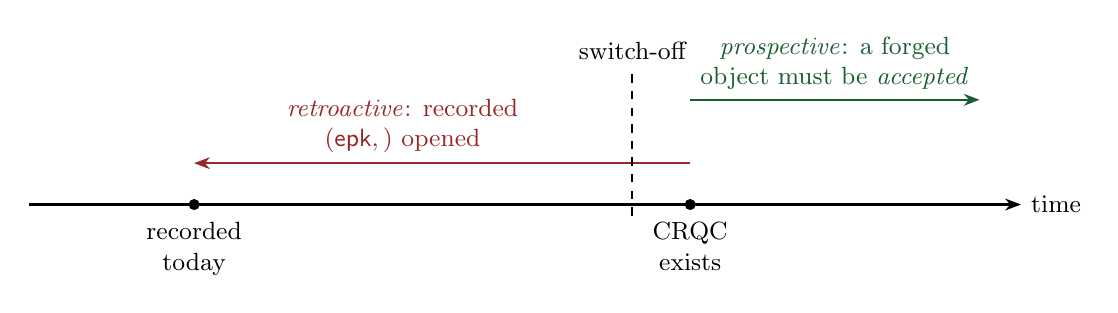
\begin{tikzpicture}[x=1.05cm, y=0.7cm, >={Stealth[length=2mm]},
  lab/.style={font=\small, align=center}]
\draw[->, thick] (0,0) -- (12,0) node[right, font=\small] {time};
\fill (2,0) circle (2pt);
\node[lab, below=3pt] at (2,0) {recorded\\today};
\fill (8,0) circle (2pt);
\node[lab, below=3pt] at (8,0) {CRQC\\exists};
\draw[<-, thick, arbred] (2,0.75) -- (8,0.75)
  node[pos=0.42, above, lab] {\emph{retroactive}: recorded\\
  $(\epk, \wbICenc)$ opened};
\draw[->, thick, arb] (8,1.9) -- (11.5,1.9)
  node[midway, above, lab] {\emph{prospective}: a forged\\object must
  be \emph{accepted}};
\draw[dashed, thick] (7.3,-0.2) -- (7.3,2.45) node[above, font=\small]
  {switch-off};
\end{tikzpicture}}
\end{center}
\Write
\begin{itemize}
  \item ``CRQC = a quantum computer running Shor at scale: discrete logs
    in polynomial time; every group assumption falls.''
  \item Retroactive: ``exploitable the day the adversary exists''.
  \item Prospective: ``a validator must \emph{accept} the forgery;
    switch off first''.
  \item ``Orchard, both pools: one retroactive break.''
\end{itemize}
\newpage
\Say
\begin{itemize}
  \item Every group assumption in this workshop falls together; the
    useful axis is reversibility, not the calendar.
  \item Retroactive: what is on chain today is exploitable the day the
    adversary exists, and no later consensus change can help.
    Prospective: a validator must accept the forged object, so
    switching off first removes acceptance.
  \item Orchard's one retroactive break is the note encryption;
    everything else on the integrity stack is prospective.
  \item Bitcoin has no ciphertext to open, but a silent-payment scan key
    has the retroactive shape; an exposed public key is the prospective
    case.
\end{itemize}
\end{board}

\begin{board}{Retroactive: harvest now, decrypt later}{none --- privacy
  of the note}
\Write
\begin{itemize}
  \item Published per Action: $(\epk, \wbICenc)$.
  \item The one discrete-log link: Diffie--Hellman between \esk{} and
    \pkd; ``KDF and AEAD above it are symmetric''.
  \item The attack, as one line:
    \[
    \ivk = \log_{\gd}\pkd
    \quad\Longrightarrow\quad
    K = \mathrm{KDF}\bigl([\ivk]\,\epk, \ldots\bigr)
    \]
  \item ``One logarithm per \ivk{} scope, then the recipient's own
    trial-decryption loop over the recorded chain.''
  \item Recovered per note: $(d, v, \mathsf{rseed}, \mathsf{memo})$ ---
    past and future.
  \item Example: Bob's $1.5$ ZEC and the memo.
\end{itemize}
\newpage
\Say
\begin{itemize}
  \item Confidentiality rests on exactly one discrete-log link; the KDF
    and the AEAD are not the weak layer.
  \item Out comes every note ever sent to any diversified address
    sharing that \ivk, past and future alike.
  \item Whoever else holds Bob's address can one day read the $1.5$ ZEC
    and the memo: storage today, the logarithm later.
\end{itemize}
\end{board}

\begin{board}{Retroactive: two limits, and the bin}{none --- privacy of
  the note}
\Write
\begin{itemize}
  \item Limit 1: ``\ivk{} views, never spends; \asksym{} not exposed''.
  \item Limit 2: ``keyed by the address: no $(d, \pkd)$, no base \gd,
    no target \pkd''.
  \item Bin: \emph{open problem} --- ``nothing deployed or specified
    protects even future ciphertexts (ZIP-2005 non-requirement);
    recorded ones unrepairable''.
  \item Bitcoin column: silent payments --- one logarithm of the scan
    key replays the scan; amount and memo never hidden.
\end{itemize}
\newpage
\Say
\begin{itemize}
  \item The viewing capability confers no spend authority; exposure of
    \asksym{} is the prospective case.
  \item Without $(d, \pkd)$ the adversary has neither the base nor the
    target, and no known efficient generic route recovers the plaintext
    from the ciphertext alone.
  \item Recorded ciphertexts are unrepairable by construction: any
    upgrade alters only ciphertexts not yet created.
  \item Silent payments: one logarithm of the published scan key links
    everything that address ever received.
\end{itemize}
\end{board}

\begin{board}{Prospective: the discrete-log integrity stack}{all four}
{\centering\small
\begin{tabular}{@{}p{0.27\textwidth}p{0.69\textwidth}@{}}
\toprule
construction & with the generators' logarithms known \tabularnewline
\midrule
\raggedright Sinsemilla binding (\NoteCommit, \CommitIvk) &
\raggedright a second note under an on-chain \cmx{} --- balance breaks
silently, turnstile-bounded; a second $(\aksym, \nksym)$ for the same
\ivk{} --- a spendability forgery \tabularnewline
\addlinespace[2pt]
\raggedright Value commitment, binding signature &
\raggedright any \cvsym{} reopens to any value; a solved $\mathsf{bvk}$
forges the signature --- inflation, turnstile-bounded \tabularnewline
\addlinespace[2pt]
\raggedright Spend authorisation (RedPallas) &
\raggedright one logarithm of \aksym{} or of any published \rksym{}
forges spend authority; theft still needs a witness or a proof forgery
\tabularnewline
\addlinespace[2pt]
\raggedright Proof soundness (IPA on Vesta) &
\raggedright commitment equivocation; the knowledge-soundness reduction
no longer holds \tabularnewline
\bottomrule
\end{tabular}\par}
\Write
``recorded \cvsym{} perfectly hiding; $\alpha$ masks \rksym; transcripts
simulatable; without the address, no generic route to these secrets''.
\Say
Shor invalidates the reductions; it does not turn them into attacks by
itself. Each construction has its own concrete consequence.
\end{board}

\begin{board}{Why the integrity breaks are prospective}{all four}
\Write
\begin{itemize}
  \item ``A forged object --- proof, signature, commitment opening ---
    must be \emph{accepted}, at current height under current rules.''
  \item ``Switch off before the CRQC $\Rightarrow$ no acceptance; history
    anchored by chain work and upgrade policy.''
  \item Residue 1: switch-off must precede the \emph{first} forgery.
  \item Residue 2: honest funds inside a disabled pool need a way out
    $\Rightarrow$ ZIP-2005.
\end{itemize}
\Say
\begin{itemize}
  \item A forged object is worthless until a node takes it; that is what
    makes the four rows prospective.
  \item An attack landed inside the window is not repaired afterwards.
  \item Bitcoin has the same shape: ECDSA and Schnorr fall to one
    logarithm of an exposed public key, and the forged spend must still
    be mined.
\end{itemize}
\end{board}

\begin{board}{The symmetric backbone survives}{authorised}
\Write
\begin{itemize}
  \item BLAKE2b: $\mathsf{PRFexpand}$ (every key and note-randomness
    derivation), KDF, outgoing cipher key, RedPallas challenge, ZIP-244
    digests; ZIP-32 Orchard tree hardened-only.
  \item Poseidon: the nullifier PRF, keyed by \nksym{} --- a heuristic,
    classically and quantumly alike.
  \item Grover:
    \[
    2^{256} \text{ classical evaluations} \;\longrightarrow\;
    \approx 2^{128} \text{ quantum ones}
    \]
  \item ``Best implementable generic collision attack: still the
    classical parallel one.''
  \item ``Ownership stays \emph{provable} after it stops being
    \emph{enforceable}.''
\end{itemize}
\newpage
\Say
\begin{itemize}
  \item Two primitive families carry no discrete-log structure; only
    generic speedups apply.
  \item A seed holder can still prove, by re-executing the hardened
    derivations, that their keys descend from their seed --- the fact
    ZIP-2005 builds on.
  \item Bitcoin: SHA-256 and hardened BIP-32 derivation stand on the
    same ground.
\end{itemize}
\end{board}

\begin{board}{ZIP-2005: the hashed trapdoor}{exists}
\Write
\begin{itemize}
  \item The Ironwood derivation, in full:
    \[
    \rcm := \mathrm{ToScalar}\bigl(\mathsf{PRFexpand}_{\mathsf{rseed}}(
    \mathtt{0x0B} \,\|\, \gd^\star \,\|\, \pkd^\star \,\|\,
    \mathrm{LE}_{64}(v) \,\|\, \mathrm{LE}_{256}(\rho) \,\|\,
    \mathrm{LE}_{256}(\psi))\bigr)
    \]
  \item ``$137$-byte preimage --- every note field traverses BLAKE2b
    into the trapdoor''.
  \item ``Under a CRQC, \NoteCommit{} alone is not binding.''
  \item ``$\mathsf{PRFexpand}$ as a random oracle: two honest notes on
    one commitment = a collision event; bound $O(q^3/N)$, about
    $2^{-74}$ at $q = 2^{60}$.''
  \item ``Post-quantum binding \emph{provided a verifier checks the
    derivation} --- no deployed clause does.''
  \item Legacy $\mathtt{0x02}$ notes: $\mathtt{0x05} \,\|\, \rho$ only
    $\Rightarrow$ unrecoverable $\Rightarrow$ the seal.
\end{itemize}
\newpage
\Say
\begin{itemize}
  \item Sinsemilla's collision resistance is the first thing to fall,
    and \NoteCommit{} alone is then not binding. With every note field
    hashed into the trapdoor, opening one commitment to two honestly
    derived notes is a collision event with no group structure for Shor
    to exploit.
  \item The circuit checks the commitment, not the derivation behind
    its trapdoor; that check is the Recovery Statement's job.
  \item Legacy notes are unrecoverable, and that is why the Orchard pool
    is sealed.
  \item Bitcoin ownership is a public key exposed at spend; the hardened
    derivation behind it is symmetric too, but no rule reads it.
\end{itemize}
\end{board}

\begin{board}{Recoverability, not resistance}{exists; authorised}
\Write
\begin{itemize}
  \item ``Recovery Statement --- proved one day, post-quantum proof
    system, re-hashed tree''.
  \item The chain of claims, top to bottom: key derivations from
    $\mathsf{sk}$; $\ivk = \CommitIvk$; $\pkd = [\ivk]\,\gd$; $\psi$ and
    \rcm{} derivations; the commitment; a membership path; the
    nullifier; the $\alpha$ re-randomisation.
  \item Cost: $7$ BLAKE2b-512 compressions, $1$ BLAKE3 compression, $2$
    Sinsemilla commitments, $2$ Pallas scalar multiplications, a Merkle
    path.
  \item ``binding only; privacy unchanged; opens no ciphertext''.
\end{itemize}
\Say
\begin{itemize}
  \item The Recovery Statement is what a holder would one day prove: with
    no group assumption, that one seed derives a committed note, its
    nullifier and its \rksym.
  \item The cost is mostly hashing.
  \item It opens no ciphertext; the harvested corpus is untouched by it.
\end{itemize}
\end{board}

\begin{board}{ZIP-2005: deployed, specified, designed, open}
  {exists; authorised}
{\centering\small
\begin{tabular}{@{}p{0.27\textwidth}p{0.69\textwidth}@{}}
\toprule
bin & content \tabularnewline
\midrule
\raggedright\emph{specified and deployed} &
\raggedright the $\mathtt{0x03}$ derivation and the three seal rules
--- every Ironwood output is recoverable \tabularnewline
\addlinespace[2pt]
\raggedright\emph{specified, undeployed} &
\raggedright the quantum-key path ($\mathsf{qsk}$, $\mathsf{qk}$); no
consensus rule \tabularnewline
\addlinespace[2pt]
\raggedright\emph{designed, unspecified} &
\raggedright the Recovery Protocol --- proof system, collapsing tree
hash, linking commitments all unfixed \tabularnewline
\addlinespace[2pt]
\raggedright\emph{open} &
\raggedright post-quantum proofs and signatures for ongoing spends; the
switch-off schedule \tabularnewline
\bottomrule
\end{tabular}\par}
\Write
``Sprout, Sapling, Orchard-pool notes: unrecoverable $\Rightarrow$ sweep
into Ironwood, ongoing; change already routed there''. ``The harvested
corpus accrues now.''
\Say
The harvested corpus is the one cost the strategy cannot answer.
\end{board}

\begin{board}{Beyond the core: what each one adds}{all four unchanged}
{\centering\small
\begin{tabular}{@{}p{0.13\textwidth}p{0.52\textwidth}p{0.27\textwidth}@{}}
\toprule
name & what it adds & Bitcoin \tabularnewline
\midrule
FROST & \raggedright $t$-of-$n$ custody of \asksym; the aggregate is an
ordinary spend-auth signature under \rksym{} &
\raggedright a Taproot FROST suite \tabularnewline
\addlinespace[2pt]
FlyClient & \raggedright logarithmic chain proofs, difficulty-weighted
sampling over a Merkle mountain range &
\raggedright SPV fetches every header \tabularnewline
\addlinespace[2pt]
ZSA & \raggedright issued assets, per-asset notes and value
commitments, issuance, burn &
\raggedright Elements' issued assets \tabularnewline
\addlinespace[2pt]
Crosslink & \raggedright proof of work kept, plus a trailing BFT
finality layer cross-linked with it &
\raggedright confirmations, never finality \tabularnewline
\bottomrule
\end{tabular}\par}
\Write
``none of the four adds privacy: custody, chain verification, assets,
settlement --- hiding unchanged''.
\end{board}

\begin{board}{Beyond the core: the bins}{all four unchanged}
{\centering\small
\begin{tabular}{@{}p{0.13\textwidth}p{0.83\textwidth}@{}}
\toprule
name & bin, as the volume states it \tabularnewline
\midrule
FROST & \raggedright \emph{specified} --- RFC 9591 and ZIP-312 (Draft);
shipped as a library; no consensus rule names it; key generation in no
ZIP \tabularnewline
\addlinespace[2pt]
FlyClient & \raggedright commitment \emph{deployed and
consensus-critical} (ZIP-221, its root committed in every header since
Heartwood); proofs \emph{unbuilt} --- no server serves one, no client
asks; the Zcash instantiation designed, not specified \tabularnewline
\addlinespace[2pt]
ZSA & \raggedright core \emph{specified} in Draft ZIPs 226 and 227; the
carrier --- v6 wire format, digests, lead byte, fees ---
\emph{unspecified} since the ZIPs that held it were withdrawn; upgrade
inclusion \emph{open} \tabularnewline
\addlinespace[2pt]
Crosslink & \raggedright \emph{design stage} --- no ZIP, nothing
activated on mainnet or testnet; a feature net runs prototype code;
construction rules \emph{designed but unspecified} \tabularnewline
\bottomrule
\end{tabular}\par}
\Write
The three bins: \emph{specified} / \emph{designed but unspecified} /
\emph{open problem}; ``deployed behaviour cites the implementation and
the specification instead''.
\end{board}

\begin{board}{Where each one sits}{all four unchanged}
\begin{center}
\resizebox{!}{0.45\textheight}{%
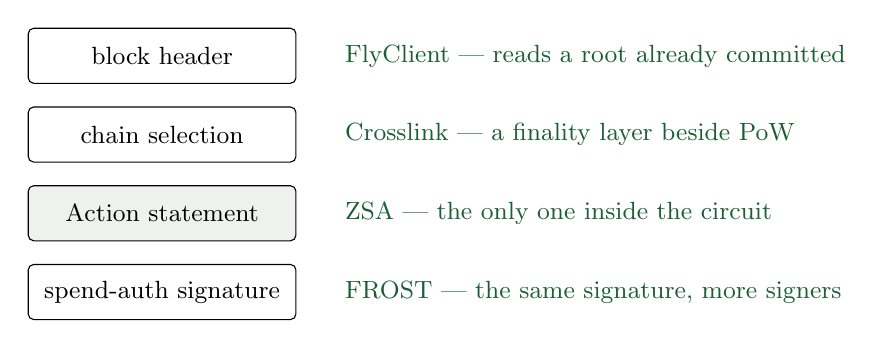
\begin{tikzpicture}[x=1cm, y=1cm, >={Stealth[length=2mm]},
  layer/.style={draw, rounded corners=2pt, minimum height=7mm,
    minimum width=34mm, font=\small, align=center},
  tag/.style={font=\small, text=arb, anchor=west}]
\node[layer] (hdr) at (0,3.0) {block header};
\node[layer] (cons) at (0,2.0) {chain selection};
\node[layer, fill=arb!8] (stmt) at (0,1.0) {Action statement};
\node[layer] (sig) at (0,0) {spend-auth signature};
\node[tag] at (2.2,3.0) {FlyClient --- reads a root already committed};
\node[tag] at (2.2,2.0) {Crosslink --- a finality layer beside PoW};
\node[tag] at (2.2,1.0) {ZSA --- the only one inside the circuit};
\node[tag] at (2.2,0) {FROST --- the same signature, more signers};
\end{tikzpicture}}
\end{center}
\Write
Beside the shaded box: ``ZSA only: Asset Base witnessed once; A1, A2 on
a per-asset commitment; A4 by variable-base multiplication; A3 dummy
skip kept for the native asset alone; split notes''. Under the stack:
``the other three leave the ten clauses as they are''.
\end{board}

\begin{board}{Takeaways: four checks, four mechanisms}{all four}
{\centering\small
\begin{tabular}{@{}p{0.15\textwidth}p{0.2\textwidth}p{0.59\textwidth}@{}}
\toprule
check & Bitcoin & Zcash \tabularnewline
\midrule
coin exists & UTXO lookup & \raggedright a commitment in an append-only
tree; membership proven under an anchor, the position a private witness
(A3) \tabularnewline
\addlinespace[2pt]
authorised & \raggedright script and signature & \raggedright the
circuit ties \rksym{} to \aksym{} (A6) and \aksym, \nksym{} to the
note's address (A7); the node's signature check under \rksym{} proves
$\rsk = \asksym + \alpha$ \tabularnewline
\addlinespace[2pt]
\raggedright not spent twice & \raggedright the UTXO is deleted &
\raggedright the nullifier, keyed by \nksym{} and seeded by $\rho$:
revealed once, rejected on repeat, unlinkable to \cmsym{} (A5)
\tabularnewline
\addlinespace[2pt]
conserved & \raggedright $\sum \mathrm{in} \ge \sum \mathrm{out}$ in the
clear & \raggedright homomorphic value commitments (A4); the binding
signature proves knowledge of $\sum \rcv$; fully shielded, valueBalance
is the fee \tabularnewline
\bottomrule
\end{tabular}\par}
\Write
``a stranger still performs all four; the note is never seen''.
\end{board}

\begin{board}{Where to read more: the Zcash Arboretum}{all four}
\Write
\begin{itemize}
  \item Foundations: \emph{Math Guide} (fields, curves, hardness);
    \emph{Crypto Guide} (the toolbox's primitives); \emph{Halo 2 Guide}
    (the proof system, in full).
  \item Deployed protocol: \emph{Consensus Guide} (the consensus part);
    \emph{Ironwood Guide} (the spine of this workshop); \emph{Wallet
    Guide} (keys, fees, the pipeline, and what the server learns).
  \item Frontier: \emph{FlyClient}, \emph{ZSA}, \emph{Crosslink} and
    \emph{FROST Guides}, each with its bins visible.
  \item ``all non-normative --- the protocol specification and the ZIPs
    are authoritative''.
\end{itemize}
\Say
None of it is normative; every volume cites the section it draws on.
\end{board}

%% ---- 12-backup.tex
\section{Backup --- optional boards}
\setlength{\emergencystretch}{2em}
\setlength{\topsep}{2pt}

\begin{board}{Sources --- the volumes, the specification, the
  ZIPs}{optional}
\Write
\begin{itemize}
  \item Volumes (non-normative): \emph{Ironwood} (the shielded critical
    path);\\ \emph{Halo 2}, \emph{Wallet}, \emph{Crypto},
    \emph{Consensus}, \emph{Math}; one row each from \emph{FROST},
    \emph{FlyClient}, \emph{ZSA}, \emph{Crosslink}.
  \item Normative: the protocol specification; the ZIPs.
  \item Final or Active: 32 keys, 203 expiry, 209 pool balances,
    213 shielded coinbase, 221 history tree, 244 digests, 316 unified
    addresses, 317 fees.
  \item Draft: 229 v6 format (the two pools), 258 the Ironwood upgrade,
    307 compact blocks, 312 FROST, 315 wallet practice, 318 migration,
    326 wallets after the seal, 374 PCZT.
  \item Proposed: 2005 quantum recoverability. Reserved stub: 2006 the
    cross-address restriction.
  \item Bins: \emph{specified} / \emph{designed but unspecified} /
    \emph{open problem}.
\end{itemize}
\newpage\Say
Every claim traces to a volume; every deployed claim to the
specification or a ZIP. The volumes are non-normative. A deployed claim
cites a specification section or a ZIP; a design-stage claim carries its
bin. Bitcoin has BIPs and no specification: the reference client's
behaviour is the definition. Here the specification is a document, and a
node implements it.
\Ask
What is normative here?
\Answer
The specification and the ZIPs; the volumes are not.
\end{board}

\begin{board}{Implementation snapshots, as the volumes cite
  them}{optional}
\Write
\begin{center}\small
\begin{tabular}{@{}l p{0.82\textwidth}@{}}
\toprule
\emph{Volume} & \emph{Snapshot} \\
\midrule
Ironwood & \textsf{orchard} 0.15.0 (the \textsf{librustzcash} pin);
  \textsf{orchard} \texttt{bef8a27} (circuit, cross-address);
  \textsf{librustzcash} \texttt{e30517e4}; \textsf{zips}
  \texttt{69610984}, rechecked at \texttt{dd1667ff} \\
Halo 2 & \textsf{halo2\_proofs} 0.3.2; \textsf{halo2\_gadgets} 0.5.0;
  \textsf{orchard} 0.15.3 \\
Wallet & \textsf{librustzcash} \texttt{e30517e4}, later snapshot
  \texttt{91f448b5}; \textsf{zips} \texttt{c6b7035} \\
  & \textsf{librustzcash} \texttt{e30517e4}; \textsf{lightwalletd}
  \texttt{61fee32e}; \textsf{Zaino} \texttt{0e057e22}; \textsf{zips}
  \texttt{6961098} \\
Consensus & \textsf{zips} \texttt{69610984}; \textsf{zebra}
  \texttt{fa7657f1c}; \textsf{librustzcash} \texttt{e30517e43};
  rechecked at \textsf{zips} \texttt{e753a6a3} \\
\bottomrule
\end{tabular}
\end{center}
\Say
Each volume pins the implementation it cites; this table answers
``which version?'' for four of them. A Bitcoin Core release number does
the same job: a claim about a default is a claim about one version.
\end{board}

\begin{board}{Implementation snapshots, continued}{optional}
\Write
\begin{center}\small
\begin{tabular}{@{}l p{0.82\textwidth}@{}}
\toprule
\emph{Volume} & \emph{Snapshot} \\
\midrule
FROST & \textsf{frost} \texttt{0966bd1}; \textsf{reddsa}
  \texttt{63c6ac0}; \textsf{zips} \texttt{e753a6a3} \\
FlyClient & \textsf{zcash\_history} 0.5.0; \textsf{zips}
  \texttt{e753a6a3} \\
ZSA & \textsf{zips} \texttt{69610984}, rechecked at \texttt{e753a6a3} \\
Crosslink & tfl-book \texttt{fe6e1d6}; \textsf{zips} \texttt{e753a6a} \\
Crypto & no baseline pin; one design-stage cite, the \textsf{orchard}
  fork \texttt{cf801a5} (ZSA issuance) \\
Math & no implementation pin; instances cite the specification \\
\bottomrule
\end{tabular}
\end{center}
\Say
The frontier volumes pin the same way: FROST, FlyClient and Crosslink
each pin an artefact and a zips checkout; ZSA pins a zips checkout and
its recheck. Two volumes pin no deployed implementation: the Crypto
Guide has one design-stage cite only; the Math Guide's instances cite the
specification.
\end{board}

\begin{board}{Scope}{optional}
\Write
\begin{itemize}
  \item A wallet default = the snapshot the volume cites, not every
    wallet.
  \item A node rail = Zebra, named only for the reorg window and the
    tie-break.
  \item Three toys: a prime-order group (balance); the $\F_{97}$ circuit
    (the proof system); the additive $\mathbb{Z}_{97}$ stand-in (the IPA
    fold, no discrete-log hardness). One mechanism each; no soundness
    estimated.
  \item Bins: \emph{specified} (a published artefact pins it down);
    \emph{designed but unspecified} (an informal source describes it);
    \emph{open problem} (no artefact exists).
  \item A deployed rule may still carry a Draft ZIP: bin and deployment
    tracked separately.
\end{itemize}
\Say
Every default in this workshop was one version's default. Each toy
isolated one mechanism; none estimates soundness. The Bitcoin contrast
is a BIP's status field; here a deployed rule may still carry a Draft
ZIP, so bin and deployment are tracked separately.
\Ask
Which toy had no discrete-log hardness?
\Answer
The additive $\mathbb{Z}_{97}$ stand-in for the IPA fold.
\end{board}

\begin{board}{The Pasta field discipline --- where each object
  lives}{optional}
\Write
\begin{center}\small
\begin{tabular}{@{}l l l@{}}
\toprule
\emph{lives in} & \emph{elements} & \emph{role} \\
\midrule
\Fpv{} (Pallas \emph{scalar} field) &
  $\asksym, \rivk, \rcm, \rcv, \alpha, \rsk, \esk, \mathsf{bsk}$ &
  multiply points \\
\Fpp{} (Pallas \emph{base} field) &
  $\nksym, \rho, \psi, \ivk, \cmx, \nfsym$ &
  the circuit's native field \\
$\Ep(\Fpp)$ (Pallas points) &
  $\aksym, \rksym, \gd, \pkd, \epk, \cmsym, \cvsym$ &
  group elements \\
bit strings &
  $\mathsf{sk}, \mathsf{rseed}, \dk, \ovk$ ($256$); $d$ ($88$) &
  keys, seeds, the diversifier \\
\bottomrule
\end{tabular}
\end{center}
\begin{itemize}
  \item One rule: multiplies a point $\Rightarrow$ scalar modulo the
    group order $p_{\Vesta}$; hashed or compared by the circuit
    $\Rightarrow$ base-field element; consumed by BLAKE2b $\Rightarrow$
    byte string.
  \item Two base-field elements act as scalars: $\pkd = [\ivk]\,\gd$
    and the nullifier's $F_{\nksym}(\rho) + \psi$ --- valid because
    $p_{\Pallas} < p_{\Vesta}$ (both $255$ bits).
  \item Bitcoin's secp256k1: coordinates modulo $p$, scalars modulo $n$;
    ECDSA $r := x(R) \bmod n$.
\end{itemize}
\newpage\Say
One rule sorts every symbol of the workshop. Two elements cross the
line, $\ivk$ and $F_{\nksym}(\rho) + \psi$, and one inequality makes
that legal: every base-field element is below the group order. Bitcoin
makes the same move once, in ECDSA's $r := x(R) \bmod n$; nothing
recomputes it inside a proof.
\Ask
Why may $\ivk$, a base-field element, multiply a point?
\Answer
Because $p_{\Pallas} < p_{\Vesta}$: every base-field element is a valid
scalar.
\end{board}

\begin{board}{The Pasta field discipline --- the two primes}{optional}
\Write
\begin{gather*}
p_{\Pallas} = 2^{254} + \mathtt{0x224698fc094cf91b992d30ed00000001},\\
p_{\Vesta}  = 2^{254} + \mathtt{0x224698fc0994a8dd8c46eb2100000001}
\end{gather*}
\begin{itemize}
  \item The cycle: $\#\Ep_{\Pallas}(\Fpp) = p_{\Vesta}$ and
    $\#\Ep_{\Vesta}(\Fpv) = p_{\Pallas}$, both prime, cofactor $1$.
  \item Both $p - 1$ carry exactly $2^{32}$; the Action circuit uses
    $2^{11}$ rows. Both primes $\equiv 1 \bmod 3$: an order-$3$
    endomorphism.
  \item Deployed: circuit over \Fpp{}; commitments on Vesta, scalar field
    \Fpp{}; one half of the cycle, no recursion.
  \item Bitcoin's secp256k1: two-adicity $1$ (base), $6$ (scalar);
    largest domain $2$ (or $64$) points.
\end{itemize}
\newpage\Say
Each curve's scalar field is the other's base field. Power-of-two
evaluation domains go up to $2^{32}$; the order-$3$ endomorphism speeds
scalar multiplication. Recursion is not deployed; verification amortises
by batching instead.
\Ask
Why not build the circuit over secp256k1?
\Answer
Its two-adicity is $1$ (scalar field $6$): the largest power-of-two
domain has $2$ (or $64$) points, far short of $2^{11}$ rows.
\end{board}

\begin{board}{Sinsemilla --- the hash}{optional --- exists}
\Write
\begin{align*}
Q(D) &:= \GroupHash^{\G}(\texttt{z.cash:SinsemillaQ},\, D),\\
P[m] &:= \GroupHash^{\G}(\texttt{z.cash:SinsemillaS},\, \mathrm{LE}_{32}(m)),
  \qquad 0 \le m < 2^{10}
\end{align*}
\[
\mathsf{Sinsemilla}_D(M) := \mathsf{Acc}_\ell, \qquad
\mathsf{Acc}_0 := Q(D), \qquad
\mathsf{Acc}_{i+1} := (\mathsf{Acc}_i \dotplus P[m_{i+1}]) \dotplus
\mathsf{Acc}_i
\]
\begin{itemize}
  \item Chunk width $k = 10$; at most $c = 253$ chunks ($2530$ bits);
    zero-padded on the right to a multiple of $10$ bits.
  \item Table $1024$ points, shared by every domain; $Q(D)$ per domain:
    $1025$ generators, all $\GroupHash$ outputs.
  \item Per chunk: one lookup, two incomplete additions ($\dotplus$).
    A $510$-bit message: $51$ rounds.
\end{itemize}
\newpage\Say
The hash is a walk: start at $Q(D)$; per $10$-bit chunk, add the chunk's
table point, then add the old accumulator. Inside the circuit the table
is a lookup argument. SHA-256 is tuned for a CPU's word operations and
costs a constraint per bit in a circuit; Sinsemilla is tuned for the
circuit that must recompute it.
\Ask
How many rounds does a $510$-bit message cost?
\Answer
Fifty-one: one lookup and two incomplete additions per $10$-bit chunk.
\end{board}

\begin{board}{Sinsemilla --- the commitment and its short
  forms}{optional --- exists}
\Write
\begin{gather*}
\mathsf{SinsemillaCommit}_r(D, M) := \mathsf{Sinsemilla}_{D\|\texttt{-M}}(M)
  + [r]\,H_D,\\
\mathsf{ShortCommit}_r(D, M) := \Extract\bigl(\mathsf{SinsemillaCommit}_r(D,
  M)\bigr), \\
\mathsf{ShortHash}_D(M) := \Extract\bigl(\mathsf{Sinsemilla}_D(M)\bigr),
\qquad
H_D := \GroupHash^{\G}(D \,\|\, \texttt{-r},\ \varepsilon)
\end{gather*}
\begin{itemize}
  \item Instances: $\NoteCommit$ --- this commitment in its own domain, a
    point; the chain stores $\cmx$, its $x$.
  \item Key commitment $\CommitIvk$ --- $\mathsf{ShortCommit}$ over
    $\mathrm{LE}_{255}(\Extract(\aksym)) \,\|\, \mathrm{LE}_{255}(\nksym)$,
    $510$ bits, $51$ rounds.
  \item Tree node hash --- $\mathsf{ShortHash}$ over $520$ bits, $52$
    rounds.
\end{itemize}
\newpage\Say
The commitment is the hash plus one blinding term; the short forms take
the $x$-coordinate. Hiding needs no assumption: for uniform $r$ the term
$[r]\,H_D$ is uniform on the group. Binding rests on $H_D$ being
unrelated to $Q$ and the table --- Pedersen's split of message base from
blinding base.
\Ask
Which side of the commitment needs an assumption, hiding or binding?
\Answer
Binding: hiding is unconditional for uniform $r$; binding needs $H_D$
unrelated to $Q$ and the table.
\end{board}

\begin{board}{Sinsemilla beside Confidential Transactions}{optional ---
  exists}
\Write
\[
\text{CT: } [v]\,V + [r]\,R; \enspace
\text{Pedersen hash: } \textstyle\sum_{j} [m_j]\,P_j; \enspace
\text{Sinsemilla: } [2^{\ell}]\,Q(D) + \textstyle\sum_{i}
  \bigl[2^{\ell - i}\bigr]\, P[m_i].
\]
\begin{itemize}
  \item One chunk: $[2]\,Q(D) + P[m_1]$ --- a lookup, not $[m_1]\,V$.
  \item Pedersen's coefficient has become Sinsemilla's index.
\end{itemize}
\Say
CT is the one-slot Pedersen commitment; the Pedersen hash adds one
generator per chunk, so its table grows with the message. Sinsemilla
keeps the discrete-log reduction, but a chunk value selects a point from
one shared table and its position supplies the weight. In Elements a
Bulletproof range-proves the opening; here $\NoteCommit$'s opening is
recomputed inside the Action proof.
\Ask
What is a one-chunk Sinsemilla?
\Answer
The point $[2]\,Q(D) + P[m_1]$ --- the chunk indexes the table instead
of scaling a generator.
\end{board}

\begin{board}{Sinsemilla --- why a collision is a discrete
  logarithm}{optional --- exists}
\Write
\begin{gather*}
\mathsf{Sinsemilla}_D(M) = [2^{\ell}]\, Q(D) + \sum_{i=1}^{\ell}
  \bigl[2^{\ell - i}\bigr]\, P[m_i],
\qquad
\chi_j(m) := \sum_{i=1}^{\ell} 2^{\ell - i}\,[m_i = j],\\
\mathsf{Sinsemilla}_D(M) = \mathsf{Sinsemilla}_D(M') \ \Longrightarrow\
\sum_{j=0}^{2^{10}-1} \bigl[\chi_j(m) - \chi_j(m')\bigr]\, P[j] = \mathcal{O}.
\end{gather*}
\begin{itemize}
  \item Take $M \ne M'$ of equal length; $\chi_j$ taken modulo
    $p_{\Vesta}$.
  \item The bound $\ell \le 253$ keeps $2^{253} < p_{\Vesta}$: nothing
    wraps; $\chi(m)$ is injective.
\end{itemize}
\newpage\Say
Unfold the accumulator, assuming no addition exception; the $Q$ terms
cancel and a collision is a linear relation among the $P[j]$. The
relation is non-trivial because $\chi$ is injective, and a non-trivial
relation among random-oracle generators is found only by discrete
logarithms. A SHA-256 collision would falsify a heuristic; a Sinsemilla
collision computes a discrete logarithm on Pallas.
\Ask
Why does $\ell \le 253$ matter to the proof?
\Answer
It keeps $2^{253} < p_{\Vesta}$, so the weight vector $\chi(m)$ never
wraps and stays injective.
\end{board}

\begin{board}{Sinsemilla --- the collision argument's fine
  print}{optional --- exists}
\Write
\[
\mathsf{Sinsemilla}_D(M) = -\mathsf{Sinsemilla}_D(M') \ \Longrightarrow\
[2^{\ell + 1}]\, Q(D) + \sum_{j}
  \bigl[\chi_j(m) + \chi_j(m')\bigr]\, P[j] = \mathcal{O}
\]
\begin{itemize}
  \item The coefficient $2^{\ell + 1} \ne 0 \bmod p_{\Vesta}$:
    non-trivial whether or not any chunk differs.
  \item Blinded forms: subtracting two openings adds $[r - r']\,H_D$ (or
    $[r + r']\,H_D$).
  \item Fixed length is load-bearing: every deployed use fixes its input
    length.
\end{itemize}
\Say
The short forms identify $P$ with $-P$, which adds this $-$ case.
Blinding does not weaken the argument: two distinct notes cannot share
$\cmsym$, nor $\cmx$. An undefined incomplete addition is an equality
between accumulator points, itself a relation among the same generators.
A Bitcoin hash is used at every length; here each domain hashes one
fixed length.
\Ask
What breaks if the input length is not fixed?
\Answer
Zero-padding lets two messages of different bit-lengths collide with no
relation among the generators at all.
\end{board}

\begin{board}{The seal --- three rules, in full}{optional --- conserved}
\Write
\begin{enumerate}
  \item \textbf{No issuance.} Coinbase: \emph{empty} Orchard component.
  \item \textbf{No circulation.} Every Orchard-pool Action:
    $\mathsf{enableCrossAddress} = 0$ --- enforced by the Action-circuit
    verifying key, selected by branch.
  \item \textbf{No entry.} Per transaction:
    $v_{\mathrm{balance}}^{\mathsf{Orchard}} \ge 0$.
\end{enumerate}
All three bind every transaction \emph{regardless of its version}
(ZIP-258).
\Say
Net value may leave the pool, never enter. The second rule lives in the
circuit, so a v5 transaction cannot bypass it: an Orchard-pool spend can
pay only its own receiver. The motive is recoverability: lead-byte
$\mathtt{0x02}$ notes cannot be recovered after a quantum break, so
consensus stops their circulation and funnels the value out. Bitcoin
retires no output type; an early P2PK coin is spendable today.
\Ask
Which of the three rules lives in the circuit?
\Answer
No circulation: the verifying key, selected by branch, enforces
$\mathsf{enableCrossAddress} = 0$.
\end{board}

\begin{board}{The cross-address restriction, A10, in full}{optional ---
  conserved}
\Write
With $\delta := \mathsf{disableCrossAddress}$ and $x(\cdot), y(\cdot)$
the affine coordinates of a Pallas point:
\begin{gather*}
\delta \cdot \bigl(x(\gd_{\mathrm{old}}) - x(\gd_{\mathrm{new}})\bigr) = 0,
\qquad
\delta \cdot \bigl(y(\gd_{\mathrm{old}}) - y(\gd_{\mathrm{new}})\bigr) = 0,\\
\delta \cdot \bigl(x(\pkd_{\mathrm{old}}) - x(\pkd_{\mathrm{new}})\bigr) = 0,
\qquad
\delta \cdot \bigl(y(\pkd_{\mathrm{old}}) - y(\pkd_{\mathrm{new}})\bigr) = 0.
\end{gather*}
\begin{itemize}
  \item Public inputs, in order: $\mathsf{anchor}$; $\cvsym$ ($x$, $y$);
    $\nfsym$; $\rksym$ ($x$, $y$); $\cmx$; $\mathsf{enableSpends}$;
    $\mathsf{enableOutputs}$; $\delta$ (index $9$) --- ten in all.
  \item Same gate shape as A3: $v_{\mathrm{old}} \cdot (\mathsf{root} -
    \mathsf{anchor}) = 0$.
  \item Flags byte: $\mathtt{0b001}$ spends, $\mathtt{0b010}$ outputs,
    $\mathtt{0b100}$ cross-address; canonical $\mathtt{0b011}$ Orchard
    pool, $\mathtt{0b111}$ Ironwood.
\end{itemize}
\newpage\Say
With $\delta \ne 0$ the four rows make the receivers equal as full
points. On the wire the polarity is reversed: bit $2$ of the flags byte
is $\mathsf{enableCrossAddress}$, and bit $2 = 0$ is what a v5 signer
treating it as reserved-zero already produces, so hardware signers keep
signing unchanged. A soft fork narrows which scripts are valid; here the
narrowing is a new verifying key selected by branch, plus one formerly
reserved bit.
\Ask
Why four equalities and not two?
\Answer
Equality in $x$ alone would identify $P$ with $-P$; $x$ and $y$ of both
$\gd$ and $\pkd$ make the receivers equal as full points.
\end{board}

\begin{board}{Spending under the restriction}{optional --- conserved}
\Write
\[
(\mathsf{addr}_{\mathrm{old}},\ v_{\mathrm{old}}) \ \longrightarrow\
(\mathsf{addr}_{\mathrm{new}} = \mathsf{addr}_{\mathrm{old}},\
 v_{\mathrm{new}} = 0), \qquad
v_{\mathrm{balance}}^{\mathsf{Orchard}} = v_{\mathrm{old}} > 0.
\]
\begin{itemize}
  \item Pay anyone by \emph{exiting}: value leaves through a positive
    $v_{\mathrm{balance}}^{\mathsf{Orchard}}$; the output slot holds a
    fabricated zero-valued note to the spent note's own receiver.
  \item Self-sends stay possible; wallets forbid sends to
    \emph{external} Orchard-pool receivers (ZIP-326).
\end{itemize}
\Say
An Action spends one note and creates one; A10 fixes the created note's
receiver, and the zero-valued output keeps the Orchard tree growing.
Paying an Orchard-pool receiver requires a spend at that receiver, hence
its spending key. The nearest Bitcoin concept is a covenant, which
script does not offer; here it is one gate in a fixed circuit.
\Ask
How does an Orchard-pool owner pay Bob?
\Answer
By exiting: the value leaves as a positive
$v_{\mathrm{balance}}^{\mathsf{Orchard}}$, and the Action's output is a
zero-valued note to the spent note's own receiver.
\end{board}

\begin{board}{The fabricated output, and the restriction's
  standing}{optional}
\Write
\begin{itemize}
  \item Fabricated output: $C_{\mathrm{enc}}$ = random bytes.
  \item Inside a PCZT: recipient, value, $\mathsf{rseed}$ explicit
    $\Rightarrow$ signer classifies it as a tolerable dummy.
  \item \emph{Specified}: the flag's encoding, its consensus rule, the
    verifying-key selection by branch (ZIP-229, ZIP-258).
  \item \emph{Designed but unspecified}: the semantics of ``equal
    receivers'', the flag-to-instance mapping, the dummy-spend
    treatment.
  \item ZIP-2006: a Reserved stub.
\end{itemize}
\newpage\Say
A real encryption would let any $\ivk$ holder --- a later quantum
adversary who recovered $\ivk$ from a published address included ---
decrypt the output and link the Action's nullifier to the address; that
is ZIP-326's reasoning. The restriction is deployed and enforced by
consensus, yet its owning ZIP is a stub. A Bitcoin signer sees every
output in the clear; a shielded signer needs the format to tell it which
output is a dummy.
\Ask
Why is the fabricated $C_{\mathrm{enc}}$ random rather than a real
encryption of the zero note?
\Answer
A real encryption would let an $\ivk$ holder --- a future one included
--- link the Action's nullifier to the address.
\end{board}

\begin{board}{The turnstile and migration}{optional --- conserved}
\Write
\[
\mathsf{IronwoodPoolBalance} := -\sum_{\mathrm{tx}}
  v_{\mathrm{balance}}^{\mathsf{Ironwood}}(\mathrm{tx}) \;\ge\; 0,
\qquad
v_{\mathrm{balance}}^{\mathsf{Orchard}} \ge 0 \text{ per transaction.}
\]
\begin{itemize}
  \item Migrating transaction: Orchard-pool spends with
    $v_{\mathrm{balance}}^{\mathsf{Orchard}} > 0$ $\rightarrow$
    transparent funds (fees and transparent outputs paid here)
    $\rightarrow$ $v_{\mathrm{balance}}^{\mathsf{Ironwood}} < 0$. Both
    fields cleartext.
  \item Pool balances: zero before the upgrade, never negative, summing
    to at most $\mathsf{MAX\_MONEY}$ (ZIP-209).
  \item Consensus caps nothing migration-specific; ZIP-318 recommends
    migration outputs of at most $10\,000$ ZEC.
  \item Ironwood tree capacity $2^{32}$; history tree gains three
    Ironwood fields.
\end{itemize}
\newpage\Say
The turnstile is the instrument that retired Sprout: a one-way,
publicly metered gate whose consensus content is exactly the two rules
above. Both fields are cleartext, so the amount crossing is public in
every transaction. Bitcoin keeps no per-type ledger row because every
amount is already public; the pool balance is the shielded ledger's one
public number per pool.
\Ask
Where does a migrating transaction pay its fee?
\Answer
From the transparent funds it passes through between the Orchard exit
and the Ironwood entry.
\end{board}

\begin{board}{The quantum footnote --- what Part I left out}{optional}
\Write
\begin{itemize}
  \item One external $\ivk$ opens neither the internal-scope $\ivk$ nor
    any scope whose address the adversary never learns.
  \item The $\rcm$ derivation's collision bound: classical $O(q^2/N)$
    $\rightarrow$ QROM $O(q^3/N)$ (Zhandry, compressed oracle). At $q =
    2^{60}$, $N \approx 2^{254}$: $2^{-134}$ classically, $2^{-74}$ in
    the QROM.
  \item Recovery Statement, key half: $\mathsf{BindKeys}$ ---
    $\asksym$, $\aksym$, $\nksym$ from $\mathsf{sk}$; plus $\rivk$ from
    $\mathsf{sk}$ by $\mathsf{PRFexpand}$, or from a quantum key
    $\mathsf{qk}$ = one BLAKE3 compression of $\mathsf{qsk}$;
    signatures of knowledge over the sighash.
\end{itemize}
\newpage\Say
The retroactive break is keyed by the address, not by the ciphertext.
The QROM lift costs a factor $q$. The $\mathsf{qk}$ route serves where
no single $\mathsf{sk}$ does: FROST-generated or hardware-held keys. A
forged signature under an exposed Bitcoin key must be accepted; a
forged RedPallas signature alone spends nothing here --- theft also
needs the note's witness or a proof forgery --- and the pool's exit caps
counterfeit, not theft.
\Ask
Does a recovered external $\ivk$ reach the change?
\Answer
No: change lands under the separate internal-scope $\ivk$, which the
external one does not open.
\end{board}

\end{document}
